\input{"preamble.tex"}

\addbibresource{FloerHomology.bib}

\let\Begin\begin
\let\End\end
\newcommand\wrapenv[1]{#1}

\makeatletter
\def\ScaleWidthIfNeeded{%
 \ifdim\Gin@nat@width>\linewidth
    \linewidth
  \else
    \Gin@nat@width
  \fi
}
\def\ScaleHeightIfNeeded{%
  \ifdim\Gin@nat@height>0.9\textheight
    0.9\textheight
  \else
    \Gin@nat@width
  \fi
}
\makeatother

\setkeys{Gin}{width=\ScaleWidthIfNeeded,height=\ScaleHeightIfNeeded,keepaspectratio}%

\title{
\rule{\linewidth}{1pt} \\
\textbf{
    Floer Homology
  }
    \\ {\normalsize Lectures by Akram Alishahi. University of Georgia,
Spring 2021} \\
  \rule{\linewidth}{2pt}
}
\titlehead{
    \begin{center}
  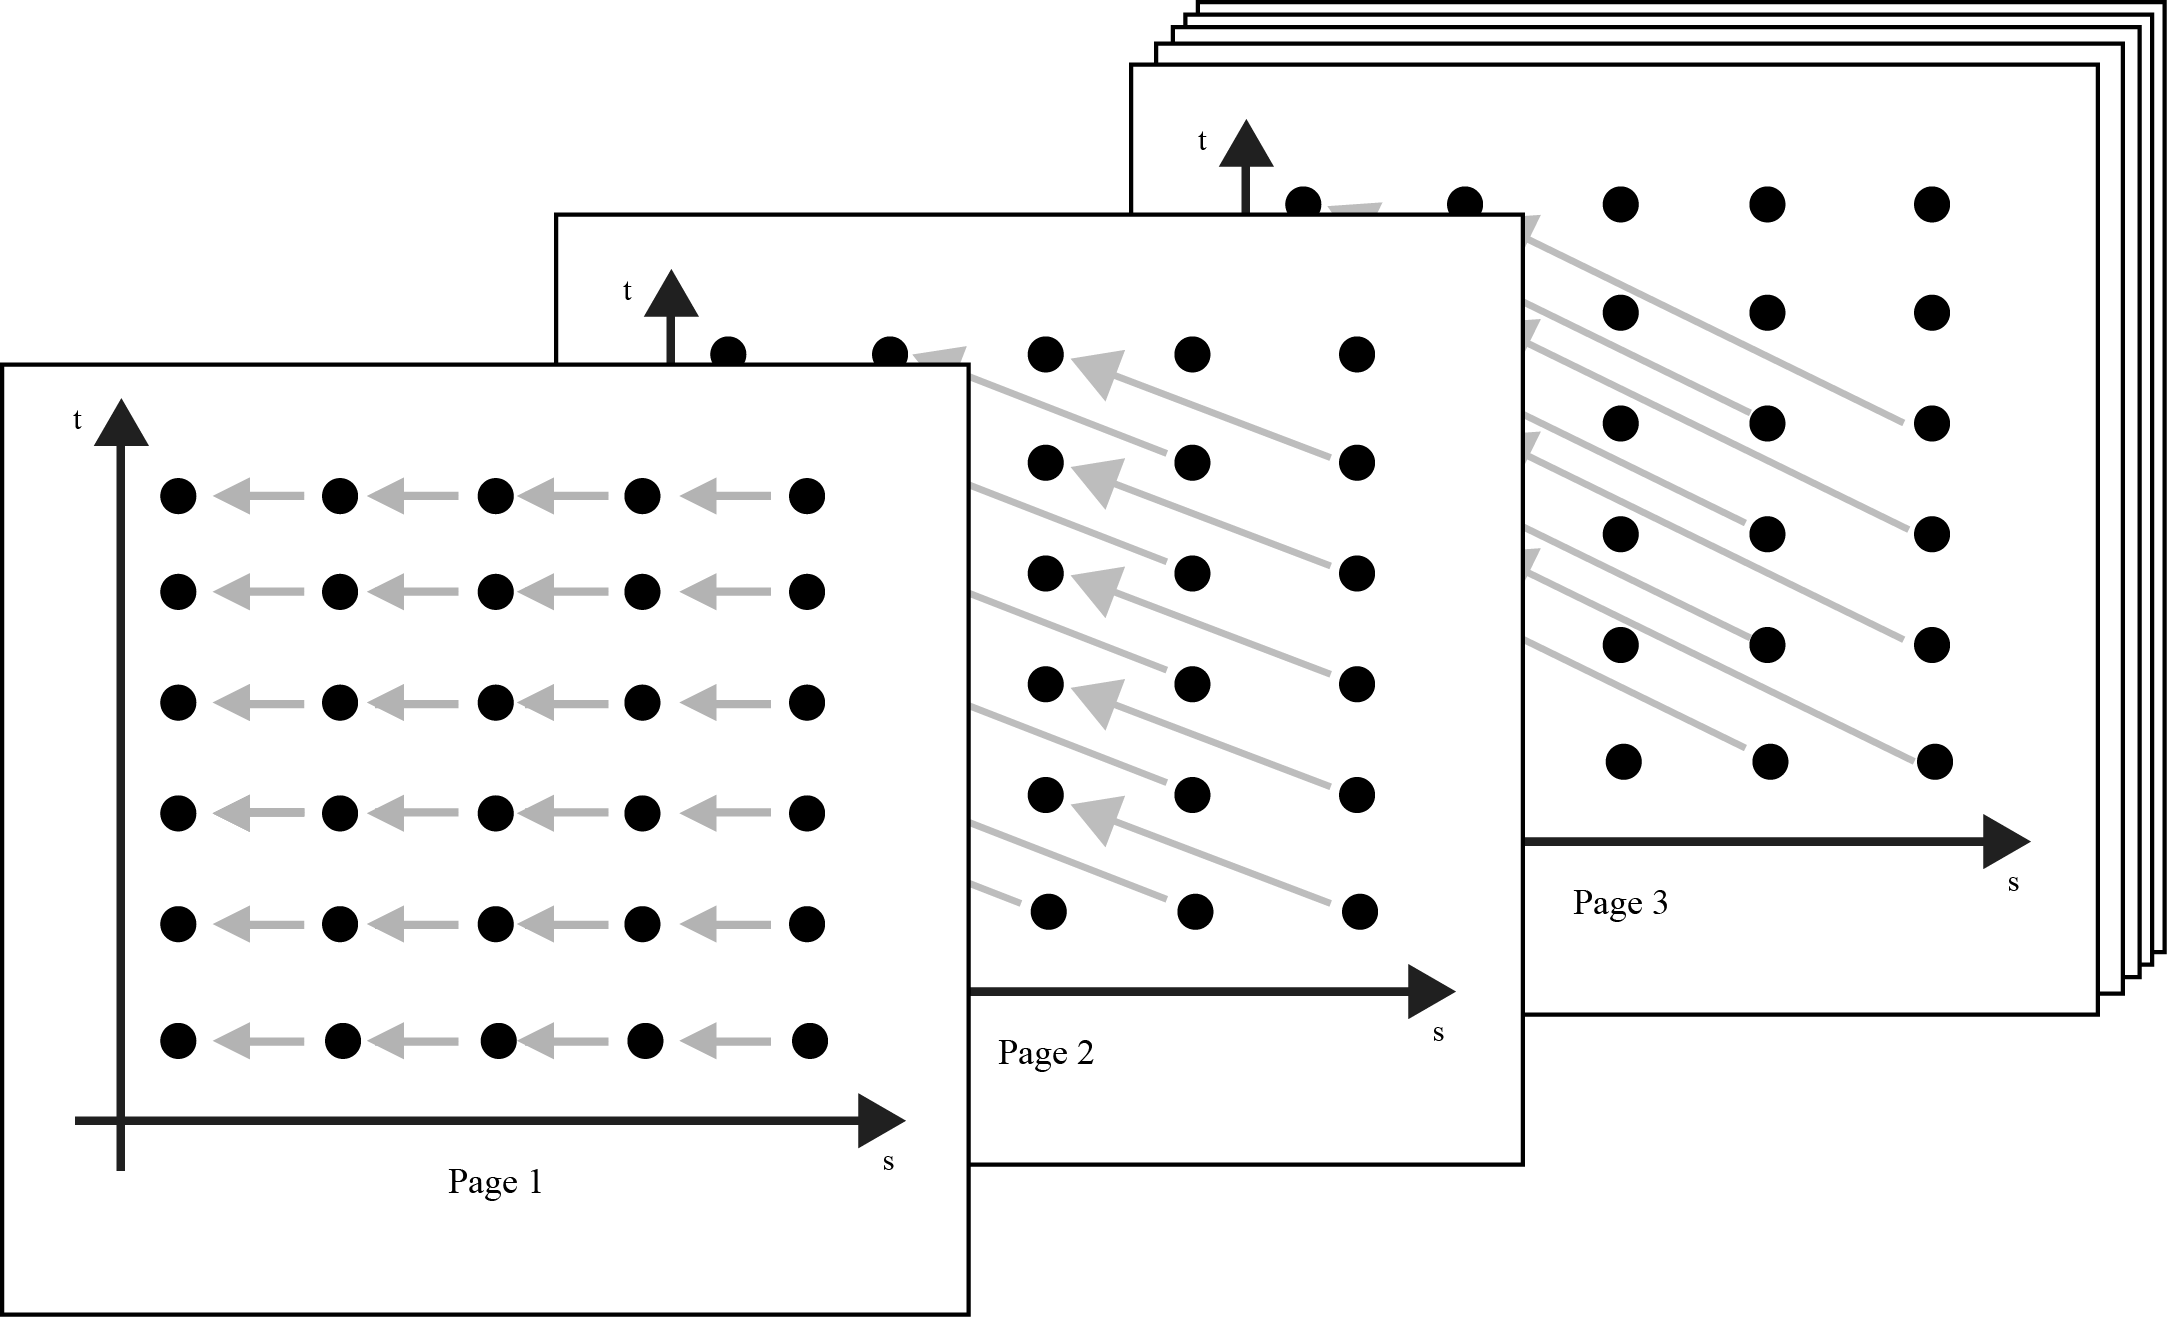
\includegraphics[width=\linewidth,height=0.45\textheight,keepaspectratio]{figures/cover.png}
  \end{center}
       \begin{minipage}{.35\linewidth}
    \begin{flushleft}
      \vspace{2em}
      {\fontsize{6pt}{2pt} \textit{Notes: These are notes live-tex'd
from a graduate course in Floer Homology taught by Akram Alishahi at the
University of Georgia in Spring 2021. As such, any errors or
inaccuracies are almost certainly my own. } } \\
    \end{flushleft}
    \end{minipage}
    \hfill
    \begin{minipage}{.65\linewidth}
    \end{minipage}
  }







\begin{document}

\date{}
\author{D. Zack Garza}
\maketitle
\begin{flushleft}
\textit{D. Zack Garza} \\
\textit{University of Georgia} \\
  \textit{\href{mailto: dzackgarza@gmail.com}{dzackgarza@gmail.com}} \\
{\tiny \textit{Last updated:} 2021-05-02 }
\end{flushleft}


\newpage

% Note: addsec only in KomaScript
\addsec{Table of Contents}
\tableofcontents
\newpage

\hypertarget{lecture-1-overview-wednesday-january-13}{%
\section{Lecture 1: Overview (Wednesday, January
13)}\label{lecture-1-overview-wednesday-january-13}}

\hypertarget{course-logistics}{%
\subsection{Course Logistics}\label{course-logistics}}

\begin{quote}
Note (DZG): Everything in this section comes from Akram!
\end{quote}

\hypertarget{description}{%
\subsubsection{Description}\label{description}}

``I am teaching a topics course about Heegaard Floer homology next
semester. Heegaard Floer homology was defined by Peter Ozsváth and
Zoltan Szabó around 2000. It is a package of powerful invariants of
smooth 3- and 4-manifolds, knots/links and contact structures. Over the
last two decades, it has become a central tool in low-dimensional
topology. It has been used extensively to study and resolve important
questions concerning unknotting number, slice genus, knot concordance
and Dehn surgery. It has been employed in critical ways to study taut
foliations, contact structures and smooth 4-manifolds. There are also
many rich connections between Heegaard Floer homology and other manifold
and knot invariants coming from gauge theory as well as representation
theory. We will learn the basic construction of Heegaard Floer homology,
starting with the definition of the 3-manifold and knot invariants. In
the second half of this course, we will turn to computations and
applications of the theory to low-dimensional topology and knot theory.
In particular, several numerical invariants have been defined using this
homological invariants. At the end of the semester, I would expect each
one of you to learn the construction of one of these invariants (of
course with my help) and present it to the class.''

\hypertarget{expository-papers}{%
\subsubsection{Expository Papers}\label{expository-papers}}

\begin{itemize}
\tightlist
\item
  \autocite{G} J. Greene,
  \href{https://www.ams.org/journals/notices/202101/rnoti-p19.pdf}{Heegaard
  Floer homology}
\item
  \autocite{H} J. Hom,
  \href{https://arxiv.org/pdf/2008.01836.pdf}{Lecture notes on Heegaard
  Floer homology}
\item
  \autocite{L} R. Lipshitz,
  \href{https://arxiv.org/abs/1411.4540}{Heegaard Floer homologies}
\item
  \autocite{M} C. Manolescu, \href{https://arxiv.org/abs/1401.7107}{An
  introduction to knot Floer homology}
\item
  \autocite{OS-1} P. Ozsváth and Z. Szabó,
  \href{https://web.math.princeton.edu/~petero/Introduction.pdf}{An
  introduction to Heegaard Floer homology}
\item
  \autocite{OS-2} P. Ozsváth and Z. Szabó,
  \href{https://web.math.princeton.edu/~petero/Lectures.pdf}{Lectures on
  Heegaard Floer homology}
\item
  \autocite{OS-3} P. Ozsváth and Z. Szabó,
  \href{https://arxiv.org/pdf/math/0403029.pdf}{Heegaard diagrams and
  holomorphic disks}
\end{itemize}

\hypertarget{research-papers}{%
\subsubsection{Research Papers}\label{research-papers}}

\begin{itemize}
\tightlist
\item
  \autocite{OSz04a} Peter Ozsváth and Zoltán Szabó, Holomorphic disks
  and topological invariants for closed three-manifolds. Ann. of Math.
  (2) 159 (2004), no. 3, 1027--1158.
  \href{https://arxiv.org/abs/math/0101206}{arXiv:math/0101206}
\item
  \autocite{OSz04b} Peter Ozsváth and Zoltán Szabó, Holomorphic disks
  and three-manifold invariants: properties and applications. Ann. of
  Math. (2) 159 (2004), no. 3, 1159--1245.
  \href{https://arxiv.org/abs/math/0105202}{arXiv:math/0105202}
\item
  \autocite{OSz04c} Peter Ozsváth and Zoltán Szabó, Holomorphic disks
  and knot invariants. Adv. Math. 186 (2004), no. 1, 58--116.
  \href{https://arxiv.org/abs/math/0209056}{arXiv:math/0209056}
\item
  \autocite{OSz06} Peter Ozsváth and Zoltán Szabó, Holomorphic triangles
  and invariants for smooth four manifolds. Adv. Math. 202 (2006), no.
  2, 326--400.
  \href{https://arxiv.org/abs/math/0110169}{arXiv:math/0110169}
\item
  \autocite{Per08} Timothy Perutz, Hamiltonian handleslides for Heegaard
  Floer homology. Proceedings of Gökova Geometry-Topology Conference
  2007, 15--35, Gökova Geometry/Topology Conference (GGT), Gökova, 2008.
  \href{https://arxiv.org/abs/0801.0564}{arXiv:0801.0564}
\end{itemize}

\hypertarget{basic-morse-theory-symplectic-geometry-and-floer-homology}{%
\subsubsection{Basic Morse Theory, Symplectic Geometry and Floer
Homology}\label{basic-morse-theory-symplectic-geometry-and-floer-homology}}

\begin{itemize}
\tightlist
\item
  \autocite{Mi-1} Milnor,
  \href{https://press.princeton.edu/books/paperback/9780691080086/morse-theory-am-51-volume-51}{Morse
  theory}
\item
  \autocite{Mi-2} Milnor,
  \href{https://press.princeton.edu/books/hardcover/9780691651132/lectures-on-the-h-cobordism-theorem}{Lectures
  on the \(h{\hbox{-}}\)cobordism theorem}
\item
  \autocite{Ca} A. Cannas da Silva.
  \href{https://www.springer.com/gp/book/9783540421955}{Lectures on
  Symplectic Geometry}
\item
  \autocite{Mc} D. McDuff,
  \href{http://www.math.stonybrook.edu/~dusa/floer8.pdf}{Floer theory
  and low-dimensional topology}
\item
  \autocite{AD} M. Audin and M. Damian,
  \href{https://link.springer.com/book/10.1007/978-1-4471-5496-9}{Morse
  theory and Floer homology}
\item
  \autocite{Hu} M. Hutchings,
  \href{https://math.berkeley.edu/~hutching/teach/276-2010/mfp.ps}{Lecture
  notes on Morse homology (with an eye towards Floer theory and
  pseudoholomorphic curves)}
\end{itemize}

\hypertarget{low-dimensional-topology}{%
\subsubsection{Low-dimensional
Topology}\label{low-dimensional-topology}}

\begin{itemize}
\tightlist
\item
  \autocite{S} N. Saveliev,
  \href{https://www.degruyter.com/view/title/121170}{Lectures on the
  topology of 3-manifolds}
\item
  \autocite{R} D. Rolfsen,
  \href{https://bookstore.ams.org/chel-346-h/}{Knots and links}
\item
  \autocite{GS} R. Gompf and A. Stipsicz,
  \href{https://bookstore.ams.org/gsm-20}{4-manifolds and Kirby
  calculus}
\item
  \autocite{L} R. Lickorish,
  \href{https://link.springer.com/book/10.1007/978-1-4612-0691-0}{An
  introduction to knot theory}
\end{itemize}

\hypertarget{suggested-topics-for-presentations}{%
\subsubsection{Suggested Topics for
Presentations}\label{suggested-topics-for-presentations}}

\begin{itemize}
\item
  \autocite{SW} S. Sarkar and J. Wang, {[}An algorithm for computing
  some Heegaard Floer homologies, Ann. of Math., 171 (2010), 1213--1236,
  \href{https://arxiv.org/abs/math/0607777}{arXiv:math/0607777}.
\item
  Grid homology from:

  \begin{itemize}
  \item
    C. Manolescu and P. Ozsváth and S. Sarkar,
    \href{https://annals.math.princeton.edu/wp-content/uploads/annals-v169-n2-p07.pdf}{A
    combinatorial description of knot Floer homology}, Ann. of Math.,
    169 (2009), 633--660,
    \href{https://arxiv.org/abs/math/0607691}{arXiv:math/0607691}.
  \item
    P. Ozsváth and A. Stipsicz and Z. Szabó,
    \href{https://bookstore.ams.org/surv-208}{Grid Homology for Knots
    and Links},

    \begin{itemize}
    \tightlist
    \item
      Also available
      \href{https://web.math.princeton.edu/~petero/GridHomologyBook.pdf}{here}
      with comment: please go and buy a hard copy, too!
    \end{itemize}
  \end{itemize}
\item
  J. Hom,
  \href{https://www.worldscientific.com/doi/abs/10.1142/S0218216517400156}{A
  survey on Heegaard Floer homology and concordance} J. of Knot Theo.
  and Its Ram.(2) 26 (2017)
  \href{https://arxiv.org/abs/1512.00383}{arXiv:1512.00383}
\item
  K. Honda and W. Kazez and G. Matić,
  \href{https://projecteuclid.org/euclid.jdg/1261495333}{On the contact
  class in Heegaard Floer homology}, J. Differential Geom. (2) 83
  (2009), 289-311,
  \href{https://arxiv.org/abs/math/0609734}{arXiv:math/0609734}
\item
  Sutured Floer homology from:

  \begin{itemize}
  \tightlist
  \item
    \autocite{L} Lipshitz expository paper listed above
  \item
    A. Juhász
    \href{https://projecteuclid.org/euclid.agt/1513796585}{Holomorphic
    discs and sutured manifolds} Algebr. Geom. Topol., (3) 6 (2006),
    1429-1457,
    \href{https://arxiv.org/abs/math/0601443}{arXiv:math/0601443}
  \item
    A. Juhász,
    \href{https://projecteuclid.org/euclid.agt/1513796824}{Knot Floer
    homology and Seifert surfaces} Algebr. Geom. Topol., (1) 8 (2008),
    603-608
    \href{https://arxiv.org/abs/math/0702514}{arxiv:math/0702514}
  \end{itemize}
\end{itemize}

\todo[inline]{Convert to bibtex?}

\hypertarget{intro-and-motivation}{%
\subsection{Intro and Motivation}\label{intro-and-motivation}}

\begin{remark}

We'll assume everything is smooth and oriented.

\end{remark}

\begin{proposition}[Osvath-Szabo (2000)]

To closed 3-manifolds \(M\) we can assign a graded abelian group
\(\widehat{HF}(M)\), which can be computed combinatorially \footnote{See
  Sarkour-Wang} . There are several variants:

\begin{itemize}
\item
  \(HF^- \in {\mathsf{grMod}}({\mathbb{Z}}_2[u])\), \footnote{This is
    the strongest variant.}
\item
  \(HF^+ \in {\mathsf{Mod}}({\mathbb{Z}}_2[u, u ^{-1} ] / u {\mathbb{Z}}_2[u])\).
\item
  \(HF^\infty \in {\mathsf{grMod}}({\mathbb{Z}}_2[u, u ^{-1} ])\),
\end{itemize}

\(HF^+\) and \(HF^\infty\) can be computed using \(HF^-\). In general,
we'll write \(HF^{-}\) to denote constructions that work with any of the
above variants.

\end{proposition}

\begin{remark}

Note that \({\mathbb{Z}}_2\) can be replaced with \({\mathbb{Z}}\), but
it's technical and we won't discuss it here. For the first half of the
course, we'll just discuss \(\widehat{HF}\), and we'll discuss the
latter 3 in the second half.

\end{remark}

\hypertarget{geometric-information}{%
\subsection{Geometric Information}\label{geometric-information}}

\begin{remark}

These invariants can be used to compute the \textbf{Thurston seminorm}
of a 3-manifold:

\end{remark}

\begin{definition}[Thurston Seminorm]

A homology class \(\alpha\in H_2(M)\) can be represented as
\(\alpha\in [S]\) for \(S\) a closed surface whose fundamental class
represents \(\alpha\) where \(S = \bigcup_{i=1}^n S_i\) can be a union
of closed embedded surfaces \(S_i\). Then we first compute
\begin{align*}
\max\left\{{0, - \chi(S_i) }\right\} 
=
\begin{cases}
0 & \text{if } S_i \cong {\mathbb{S}}^2, {\mathbb{T}}^2 \\ 
\\
- \chi(S_i) = 2g(S_i) - 2  & \text{ else} .
\end{cases}
.\end{align*}
Note that the max checks if \(\chi\) is positive. Then define
\begin{align*}
{\left\lVert { \alpha } \right\rVert} \coloneqq\min_S \qty{ \sum_{i=1}^n 
\max\left\{{0, - \chi(S_i) }\right\} }
,\end{align*}
where we sum over the embedded subsurfaces and check which overall
surface gives the smallest norm.

\end{definition}

\begin{remark}

Note that this can't be a norm, since if
\({\mathbb{S}}^2, {\mathbb{T}}^2 \in [S] \implies {\left\lVert {\alpha } \right\rVert}= 0\).

\end{remark}

\begin{theorem}[Osvath-Szabo]

\(HF\) detects \footnote{What does ``detect'' mean? This is slightly
  technical.} the Thurston seminorm, and there is a splitting as
groups/modules
\begin{align*}
HF^{-}(M) = \bigoplus _{\mathfrak{s} \in {\operatorname{Spin}}^c(M)} HF^{-}(M, S) 
\end{align*}
where \(S \in {\operatorname{Spin}}^c(M)\) is a \textbf{spin\(^c\)
structure}: an oriented 2-dimensional vector bundle on \(M\) (up to some
equivalence).

\end{theorem}

\begin{remark}

The Thurston norm \({\left\lVert {a} \right\rVert}\) can be computed
from this data by considering a perturbed version of \(\widehat{HF}\),
denoted \(\underline{\widehat{HF}}\), in the following way: taking the
first Chern class \(c_1(\mathfrak{s}) \in H^2(M)\) (which can be
associated to every 2-dimensional vector bundle), we have
\begin{align*}
{\left\lVert { \alpha} \right\rVert} = \max_{\underline{\widehat{HF}}(M, \mathfrak{s}  ) \neq 0 }
{\left\lvert {{\left\langle { c_1(\mathfrak{s})  },~{ \alpha } \right\rangle}  } \right\rvert}
.\end{align*}

\end{remark}

\begin{slogan}

Floer homology groups split over these spin\(^c\) structures and can be
used to compute Thurston norms.

\end{slogan}

\begin{theorem}[Ni]

Given \(F \subseteq M\) with genus \(g\geq 2\), \(HF\) detects if \(M\)
\emph{fibers} over \(S^1\) with \(F\) as a fiber, i.e.~there exists a
fiber bundle

\begin{center}
\begin{tikzcd}
F 
  \ar[r, hook] 
& 
M
  \ar[d, "\pi"] 
\\
& 
S^1 
\end{tikzcd}
\end{center}

This uses the existence of the splitting over spin\(^c\) structures and
uses \(HF^+\) in the following way: such a bundles exists if and only if
\begin{align*}
\bigoplus _{{\left\langle { c_1(\mathfrak{s}) },~{ [F] } \right\rangle}  =2g-2} HF^+(M, \mathfrak{s}) = {\mathbb{Z}}
.\end{align*}

\end{theorem}

\begin{definition}[Contact Structure]

Equivalently,

\begin{itemize}
\item
  A smooth oriented nowhere integrable 2-plane field \(\xi\), or
\item
  A 2-plane field \(\xi \coloneqq\ker( \alpha)\) where \(\alpha\) is a
  1-form such that \(\alpha\wedge d \alpha > 0\). \footnote{Note that
    wedging to a nontrivial top form is equivalent to being nowhere
    integrable here.}
\end{itemize}

\end{definition}

\begin{example}[?]

The standard contact structure on \({\mathbb{R}}^3\) is given by
\begin{align*}
\alpha\coloneqq dz - ydz
,\end{align*}
which yields the following 2-plane field \(\xi \coloneqq\ker \alpha\):

\begin{figure}
\centering
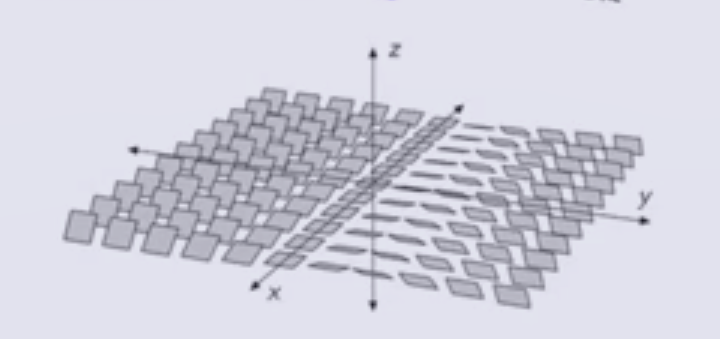
\includegraphics{figures/image_2021-01-18-23-04-19.png}
\caption{2-Plane Field in \({\mathbb{R}}^3\)}
\end{figure}

You can see that \(z=0 \implies y=0\), so the \(xy{\hbox{-}}\)plane is
in the kernel, yielding the flat planes down the middle:

\begin{figure}
\centering
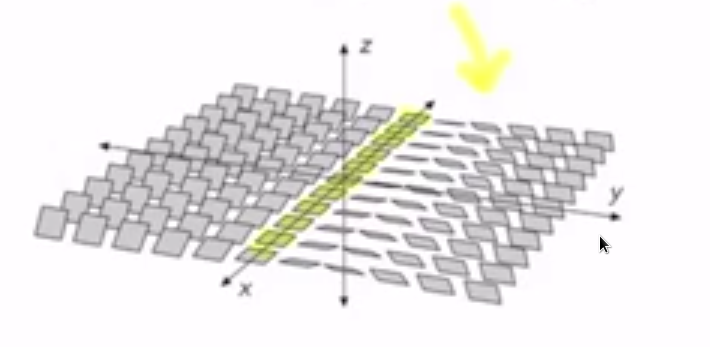
\includegraphics{figures/Flat_Planes.png}
\caption{Flat Planes}
\end{figure}

\end{example}

\begin{proposition}[Contact Class (Osvath-Szabo-Honda-Kazez-Matic)]

To each such \(\xi\) one can associate a \textbf{contact class}
\(c(\xi) \in \widehat{HF}(-M)\), where \(-M\) is \(M\) with the reversed
orientation.

\end{proposition}

\begin{remark}

This gives obstructions for two of the following important properties of
contact structures:

\begin{itemize}
\tightlist
\item
  Being \textbf{overtwisted}, or
\item
  Being \textbf{Stein fillable}.
\end{itemize}

\end{remark}

\begin{theorem}[?]

\envlist

\begin{itemize}
\tightlist
\item
  If \(\xi\) is overtwisted, then \(c(\xi) = 0\).
\item
  If \(\xi\) is Stein fillable, then \(c(\xi) \neq 0\).
\end{itemize}

\end{theorem}

\begin{remark}

We'll also discuss similar invariants for knots that were created after
these invariants for manifolds.

\end{remark}

\begin{definition}[Knots]

Recall that a \textbf{knot} is an embedding \(S^1 \hookrightarrow M\).

\begin{figure}
\centering
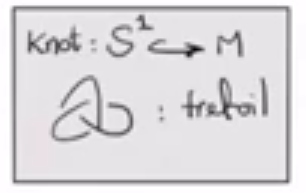
\includegraphics[width=1.5625in,height=\textheight]{figures/image_2021-01-18-23-13-07.png}
\caption{Example: the trefoil knot}
\end{figure}

\end{definition}

\begin{proposition}[Knot Floer Homology (Ozsváth-Szabó)]

Given a knot \(K \subseteq M\) a 3-manifold (e.g.~\(M = S^3\)), there is
extra algebraic structure on \(\widehat{CF}(M)\): a filtration. These
allow defining a new bigraded abelian group \(\widehat{HFK}(M, K)\)
(which is also a \({\mathbb{Z}}_2{\hbox{-}}\)vector space) that takes
includes the information of \(K\). This yields a decomposition
\begin{align*}
\widehat{HFK}(M, K) = \bigoplus _{m, a} \widehat{HFK}_m(M, K, a)
.\end{align*}

This similarly works for other variants: there is a filtration on
\(CF^-(M)\) which yields \(HFK^-(M, K)\), a bigraded
\({\mathbb{Z}}_2[u]{\hbox{-}}\)module.

\end{proposition}

\hypertarget{some-properties-of-knot-floer-homology}{%
\subsubsection{Some properties of Knot Floer
Homology}\label{some-properties-of-knot-floer-homology}}

\begin{fact}

\(\widehat{HFK}(K)\) categorifies the Alexander polynomial
\(\Delta_K(t)\) of \(K\), i.e.~taking the graded Euler characteristic
yields
\begin{align*}
\Delta_K (t) =\sum_{m, a} (-1)^m\qty{ \dim \widehat{HFK}_m(K, a) } t^a
.\end{align*}

\end{fact}

\begin{fact}

\(\widehat{HFK}(K)\) detects the \textbf{Seifert genus} of a knot
\(g(K)\), defined as the smallest \(g\) such that there exists an
embedded surface \footnote{These are referred to as \textbf{Seifert
  surfaces}.} \(F\) of genus \(g\) in \(S^3\) that bounds \(K\), so
\({{\partial}}F = K\).

\begin{example}[The Unknot]

The unknot bounds a disc, so its genus is zero:

\begin{figure}
\centering
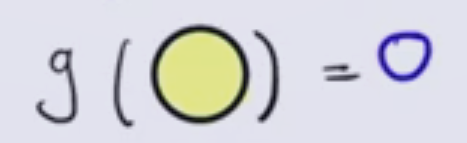
\includegraphics{figures/image_2021-01-18-23-29-23.png}
\caption{The genus of the unknot}
\end{figure}

\end{example}

\begin{exercise}[The Trefoil]

Using the ``outside'' disc on the trefoil, find 3 bands that show its
genus is 1.

\begin{figure}
\centering
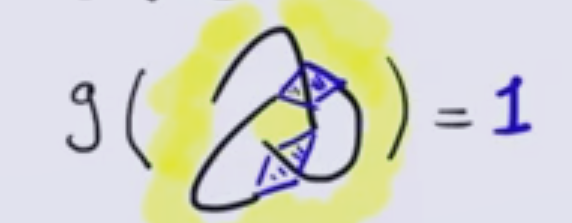
\includegraphics{figures/image_2021-01-18-23-30-49.png}
\caption{The genus of the trefoil}
\end{figure}

\end{exercise}

The genus can be computed by setting
\(\widehat{HFK}(K, a) \coloneqq\bigoplus _m \widehat{HFK}_m(K, a)\),
which yields
\begin{align*}
g(k) = \max \left\{{ a {~\mathrel{\Big|}~}\widehat{HFK}(K, a) \neq 0 }\right\}
.\end{align*}
Note that the \(a\) grading here is referred to as the \textbf{Alexander
grading}.

\end{fact}

\begin{fact}

\(\widehat{HFK}\) detects whether or not a knot is \textbf{fibered},
where \(K\) is fibered if and only if it admits an \(S^1\) family
\(F_t\) of Seifert surfaces such that
\(t\neq s\in S^1 \implies F_t \cap F_s = K\). I.e., there is a fibration
on the knot complement where each fiber is a Seifert surface:

\begin{center}
\begin{tikzcd}
\Sigma_g 
  \ar[r] 
& 
S^3\setminus K
  \ar[d, "\pi"] 
\\
& 
K 
\end{tikzcd}
\end{center}

\begin{example}[The Unknot]

The unknot is fibered by \({\mathbb{D}}^2\)s:

\begin{figure}
\centering
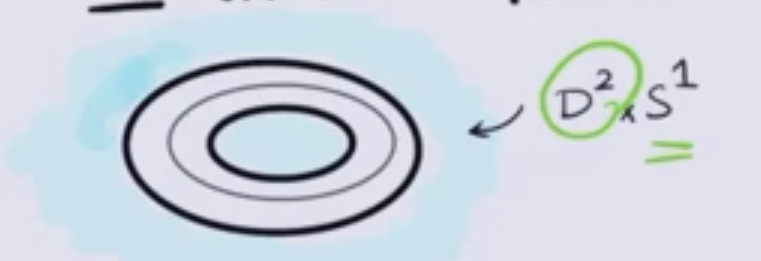
\includegraphics{figures/image_2021-01-18-23-38-35.png}
\caption{The unknot fibered by discs.}
\end{figure}

\end{example}

This is ``detected'' in the following sense: \(K\) is fibered if and
only if
\begin{align*}
\widehat{HFK}(k, g(K)) = {\mathbb{Z}}_2
.\end{align*}

\end{fact}

\begin{definition}[Slice Genus]

Let \(K \subseteq S^3\). We know \(S^3 = {{\partial}}B^4\), so we
consider all of the smoothly properly embedded surfaces \(F\) in \(B^4\)
such that \({{\partial}}F = K\) and take the smallest genus:

\begin{figure}
\centering
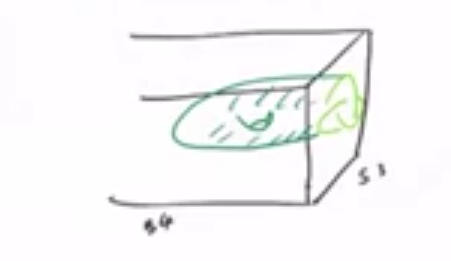
\includegraphics{figures/image_2021-01-18-23-56-35.png}
\caption{Knot in \(S^3\) bounding a surface in \(B^4\)}
\end{figure}

We thus define the \textbf{slice genus} or \textbf{4-ball genus} as
\begin{align*}
g_S(K) \coloneqq g_4(K) \coloneqq\min 
\left\{{
g(F) {~\mathrel{\Big|}~}F\hookrightarrow B^4 \text{ smootherly, properly with } {{\partial}}F = K
}\right\}
.\end{align*}

\end{definition}

\begin{exercise}[?]

Show that \(g_4(K) \leq g(K)\).

\end{exercise}

\begin{definition}[Unknotting number]

Define \(u(K)\) the \textbf{unknotting number} of \(K\) as the minimum
number of times that \(K\) must cross itself to become unknotted.

\end{definition}

\begin{example}[The Trefoil]

Consider changing the bottom crossing of a trefoil:

\begin{figure}
\centering
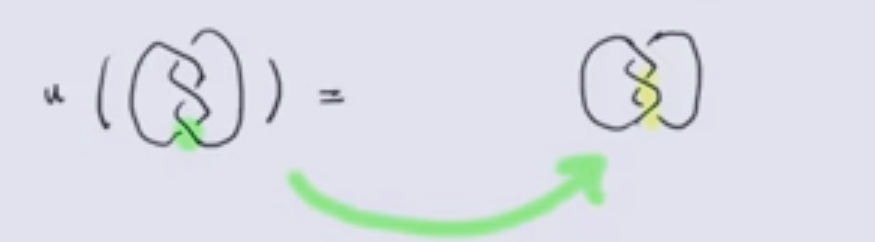
\includegraphics{figures/image_2021-01-19-00-01-14.png}
\caption{Changing one crossing in the trefoil}
\end{figure}

This in fact produces the unknot:

\begin{figure}
\centering
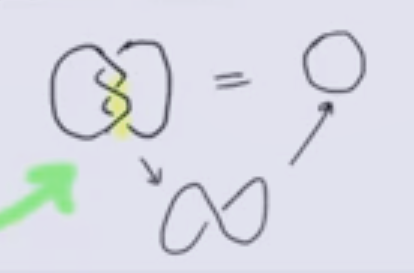
\includegraphics{figures/image_2021-01-19-00-02-00.png}
\caption{Unkink to yield the unknot}
\end{figure}

Thus \(u(K) = 1\), assuming that we know \(K \neq 0\) is not the unknot.

\end{example}

\begin{exercise}[?]

Show that \(g_f(K) \leq u(K)\).

\begin{quote}
Hint: each crossing change \(K\to K'\) yields some surface that is a
cobordism from \(K\) to \(K'\) in \(B^4\), and you can use each step to
build your surface.
\end{quote}

\begin{figure}
\centering
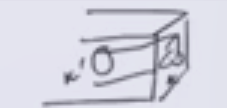
\includegraphics{figures/image_2021-01-19-00-04-13.png}
\caption{Surface between \(K\) and \(K'\)}
\end{figure}

\end{exercise}

\begin{theorem}[Ozsváth-Szabó]

Define an invariant \(\tau(K) \in {\mathbb{Z}}\) from \(\widehat{HFK}\)
such that
\({\left\lvert {\tau(K)} \right\rvert} \leq g_4(K) \leq u(K)\).

\end{theorem}

\begin{definition}[Torus Knots $T_{p, q}$ ]

Recall that we can view
\({\mathbb{T}}^2 \coloneqq{\mathbb{R}}^2/{\mathbb{Z}}^2\) where the
action is \((x, y) \xrightarrow{(m, n)} (x+m, y+m)\), i.e.~we module out
by integer translations. Then for \$p, q \textgreater{} 0 \$ coprime,
\(T_{p, q}\) is the image of the line \(y = mx\) in \({\mathbb{T}}^2\)
where \(m=p/q\).

\end{definition}

\begin{example}[$T_{2, 3}$ ]

The torus knot \(T_{2, 3}\) wraps 3 times around the torus in one
direction and twice in the other:

\begin{figure}
\centering
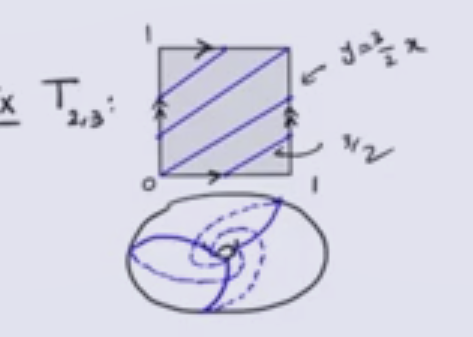
\includegraphics{figures/image_2021-01-19-00-09-51.png}
\caption{The torus knot \(T_{2, 3}\)}
\end{figure}

\end{example}

\begin{theorem}[Milnor]

\begin{align*}
g_4(T_{p, q}) = u(T_{p, q}) = { (p-1)(1-q) \over 2}
.\end{align*}

\begin{itemize}
\tightlist
\item
  First proved by Kronheimer-Mrowka
\item
  Another proof by Osvath-Szabó using Heegard Floer homology.
\end{itemize}

\end{theorem}

\begin{exercise}[?]

Show that \(u(T_{p. q}) \leq {(p-1)(q-1) \over 2}\), i.e.~torus knots
can be unknotted with this many crossing changes.

\end{exercise}

\begin{theorem}[Osvath-Szabó]

\begin{align*}
\tau(T_{p, q}) = 
{(p-1)(q-1) \over 2}
,\end{align*}

which implies
\begin{align*}
{(p-1)(q-1) \over 2}
\leq g_4(T_{p, q})
\leq u(T_{p, q})
\leq {(p-1)(q-1) \over 2}
,\end{align*}
making all of these equal.

\end{theorem}

\begin{remark}

There are better lower bounds for \(u(K)\) defined using
\(\widehat{HFK}\) which are \emph{not} lower bounds for the slice genus.
There are also other lower bounds for the slice genus with different
names (see Jen Hom's survey), some of which are stronger than \(\tau\).

\end{remark}

\begin{remark}

Another application of having these lower bounds is that we can
construct exotic (or \emph{fake}) \({\mathbb{R}}^4\)s, i.e.~4-manifolds
\(X\) homeomorphic to \({\mathbb{R}}^4\) but not diffeomorphic to
\({\mathbb{R}}^4\).

\end{remark}

\begin{remark}

All of these invariants work nicely in a \((3+1){\hbox{-}}\)TQFT: we
have invariants of 3-manifolds \(M_i\) and knots in them, so we can talk
about \textbf{cobordisms} between them: \(W^4\) a compact oriented
4-manifold with \({{\partial}}W^4 = -M_1 {\coprod}M_2\).

\begin{figure}
\centering
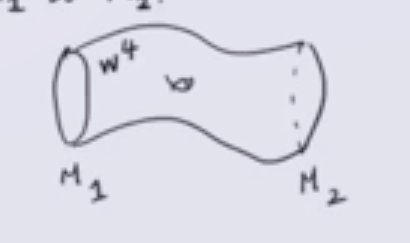
\includegraphics{figures/image_2021-01-19-00-24-31.png}
\caption{A cobordism}
\end{figure}

Osvath-Szabó define a map
\begin{align*}
F_{W, t}^{-}: HF^{-}(M_1, { \left.{{t}} \right|_{{M_1}} } ) \to HF^{-}(M_2, { \left.{{t}} \right|_{{M_2}} })
\end{align*}
using \(t\) coming from the splitting of spin\(^c\) structure which
yields an invariant of closed 4-manifolds referred to as \textbf{mixed
invariants}.

Similarly, if we have knots in 3-manifolds we can define a cobordism
\((M_1, K_1) \to (M_2, K_2)\) as \((W^4, F)\) where \(W^4\) is a
cobordism \(M_1\to M_2\) and \(F\hookrightarrow W\) is a smoothly
embedded surface that is a cobordism from \(K_1\to K_2\) with
\(F \cap M_i = K_i\) and \({{\partial}}F = -K_1 {\coprod}K_2\).

\begin{figure}
\centering
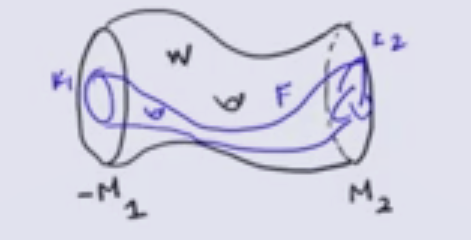
\includegraphics{figures/image_2021-01-19-00-29-04.png}
\caption{A cobordism including knots}
\end{figure}

This similarly yields a map

\begin{align*}
F_{W, F t}^{-}: HF^{-}(M_1, K_1, { \left.{{t}} \right|_{{M_1}} } ) \to HF^{-}(M_2, K_2, { \left.{{t}} \right|_{{M_2}} })
\end{align*}

\end{remark}

\begin{remark}

This smoothly embedded surface in the middle can be used to study other
smoothly embedded surfaces in 4-manifolds, which has been done recently.

\end{remark}

\hypertarget{lecture-2-tuesday-january-19}{%
\section{Lecture 2 (Tuesday, January
19)}\label{lecture-2-tuesday-january-19}}

\todo[inline]{Copy in references recommended by Akram!}

\hypertarget{constructing-heegard-floer}{%
\subsection{Constructing Heegard
Floer}\label{constructing-heegard-floer}}

\begin{remark}

For Morse Theory, there are some good exercises in Audin's book --
essentially anything other than the existence questions. The first 8
look good on p.~18.\\

Today:

\begin{enumerate}
\def\labelenumi{\arabic{enumi}.}
\item
  Overview of the construction of HF, and
\item
  A discussion of Morse Theory.
\end{enumerate}

First goal: discuss how the name ``Heegard'' fits in.

\end{remark}

\begin{definition}[Genus $g$ handlebody]

A \textbf{genus \(g\) handlebody} \(H_g\) is a compact oriented
3-manifold with boundary obtained from \(B^3\) by attaching \(g\) solid
handles (a neighborhood of an arc).

\end{definition}

\begin{example}[Attaching $g=2$ handles to a sphere]

For \(g=2\) attached to a sphere, we glue \(D^2 \times I\) by its
boundary to \(S^2\).

\begin{figure}
\centering
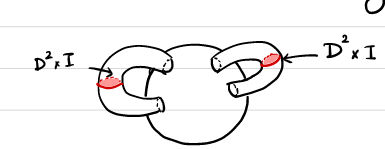
\includegraphics{figures/image_2021-01-19-00-35-48.png}
\caption{image\_2021-01-19-00-35-48}
\end{figure}

In general, \({{\partial}}H_g = \Sigma_g\) is a genus \(g\) surface, and
\(H_g \setminus{\coprod}_{i=1}^g D_i = B^3\). We can keep track of the
data by specifying \((\Sigma, \alpha_1, \alpha_2, \cdots, \alpha_g)\)
where \({{\partial}}D_i = \alpha_i\).

\begin{figure}
\centering
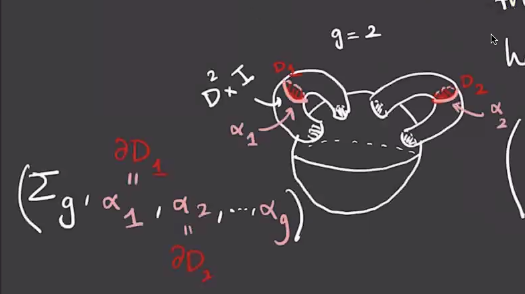
\includegraphics{figures/image_2021-01-19-11-26-35.png}
\caption{Attaching a handlebody}
\end{figure}

\end{example}

\begin{definition}[Heegard Decomposition]

A \textbf{Heegard diagram} is \(M = H_1 \cup_{{\partial}}H_2\) where
\(H_i\) are genus \(g\) handlebodies and there is a diffeomorphism
\({{\partial}}H_1 \to {{\partial}}H_2\).

\end{definition}

\begin{theorem}[?]

Every closed 3-manifold has a Heegard decomposition, although it is not
unique.

\end{theorem}

\begin{definition}[Heegard Diagram]

A \textbf{Heegard diagram} is the data
\((\Sigma_g, \alpha = \left\{{ \alpha_1, \cdots, \alpha_g}\right\}, \beta = \left\{{ \beta_1, \cdots, \beta_g}\right\})\)
where the \(\alpha\) correspond to \(H_1\) and \(\beta\) to \(H_2\) and
\(\Sigma_g = {{\partial}}H_1 = {{\partial}}H_2\).

\end{definition}

\hypertarget{lagrangian-floer-homology}{%
\subsection{Lagrangian Floer Homology}\label{lagrangian-floer-homology}}

\begin{remark}

This is essentially an infinite-dimensional version of Morse homology.

\end{remark}

\begin{definition}[Symplectic Manifold]

A \textbf{symplectic manifold} is a pair \((M^{2n}, \omega)\) such that

\begin{itemize}
\tightlist
\item
  \(\omega\) is \emph{closed}, i.e.~\(d \omega = 0\), and
\item
  \(\omega\) is \emph{nondegenerate}, i.e.~\(\wedge^n \omega \neq 0\).
\end{itemize}

\end{definition}

\begin{definition}[Lagrangian]

A \textbf{Lagrangian submanifold} is an \(L^n \subseteq M\) such that
\({ \left.{{\omega}} \right|_{{L}} } = 0\).

\end{definition}

\begin{remark}

If \(L_1 \cap L_2\) is finitely many points, case we can define a chain
complex
\begin{align*}
CF(M^{2n}, L_1, L_2) \coloneqq{\mathbb{Z}}_2[L_1 \cap L_2]
,\end{align*}
the \({\mathbb{Z}}_2{\hbox{-}}\)vector space generated by the
intersection points of the Lagrangian submanifolds. We'll define a
differential by essentially counting discs between intersection points:

\begin{figure}
\centering
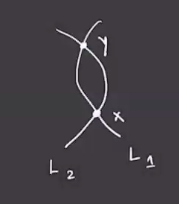
\includegraphics{figures/image_2021-01-19-11-46-38.png}
\caption{Two intersection points}
\end{figure}

We'll want to write \({{\partial}}x = c_y y + \cdots\) where \(c_y\) is
some coefficient. How do we compute it? In this case, we have half of
the boundary on \(L_1\) and half is on \(L_2\)

\begin{figure}
\centering
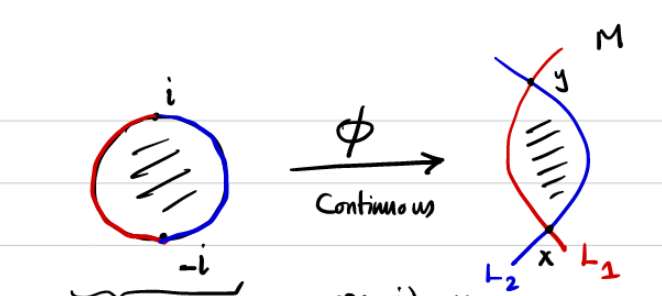
\includegraphics{figures/image_2021-01-19-00-40-08.png}
\caption{i}
\end{figure}

So we can the number of \emph{holomorphic} discs from \(x\) to \(y\).
We'll get
\({\partial}^2 = 0 \iff \operatorname{im}{\partial}\subset \ker {\partial}\),
and \(HF\) will be kernels modulo images. In more detail, we'll have
\begin{align*}
{{\partial}}x = \sum_y \sum_{\mu(\varphi) = 1} \# \widehat{\mathcal{M}} (\varphi)y &&  \widehat{\mathcal{M}}(\varphi) = \mathcal{M}(\varphi) / {\mathbb{R}}
\end{align*}
where \(\widehat{\mathcal{M}}\) will (in good cases) be a 1-dimensional
manifold with finitely many points. Note that it's not necessarily true
that \(CF\) has a grading!

Given a 3-manifold \(M^3\), we'll associate a Heegard diagram
\(\Sigma, \alpha, \beta\). Note the \(g{\hbox{-}}\)element symmetric
group acts on \(\prod_{i=1}^g \Sigma\) by permuting the \(g\)
coordinates, so we can define
\(\operatorname{Sym}^g(\Sigma) \coloneqq\prod_{i=1}^g \Sigma / S_g\).

\end{remark}

\begin{theorem}[?]

The space \(\operatorname{Sym}^g(\Sigma)\) is a smooth complex manifold
of \({\mathbb{R}}{\hbox{-}}\)dimension \(2g\).

\end{theorem}

\begin{remark}

Write
\({\mathbb{T}}_{\alpha} \coloneqq\prod_{i=1}^g \alpha_i \subseteq \prod_{i=1}^g \Sigma\)
for a \(g{\hbox{-}}\)dimensional torus; this admits a quotient map to
\(\operatorname{Sym}^g(\Sigma)\). We can repeat this to obtain
\({\mathbb{T}}_{\beta}\). Then \(HF^{-}(M)\) will be a variation of
Lagrangian Floer Homology for
\((\operatorname{Sym}^g(\Sigma), {\mathbb{T}}_{\alpha}, {\mathbb{T}}_{\beta} )\).

\end{remark}

\begin{example}[?]

Consider constructing a genus \(g=1\) Heegard diagram. Recall that
\(S^3\) can be constructed by gluing two solid torii.

\begin{figure}
\centering
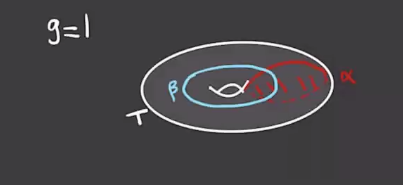
\includegraphics{figures/image_2021-01-19-12-20-16.png}
\caption{image\_2021-01-19-12-20-16}
\end{figure}

Here \((T, \alpha, \beta)\) will be a Heegard diagram for \(S^3\).

\end{example}

\begin{exercise}[?]

Show that the following diagram with \(\beta\) defined as some
perturbation of \(\alpha\) is a Heegard diagram for \(S^1 \times S^2\).

\begin{figure}
\centering
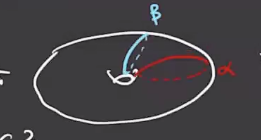
\includegraphics{figures/image_2021-01-19-12-21-56.png}
\caption{image\_2021-01-19-12-21-56}
\end{figure}

\end{exercise}

\begin{definition}[Dehn Surgery]

Consider \(M\) a 3-manifold containing a knot \(K\), we can construct a
new 3-manifold by first removing a neighborhood of \(K\) to yield
\(M\setminus N(K)\):

\begin{figure}
\centering
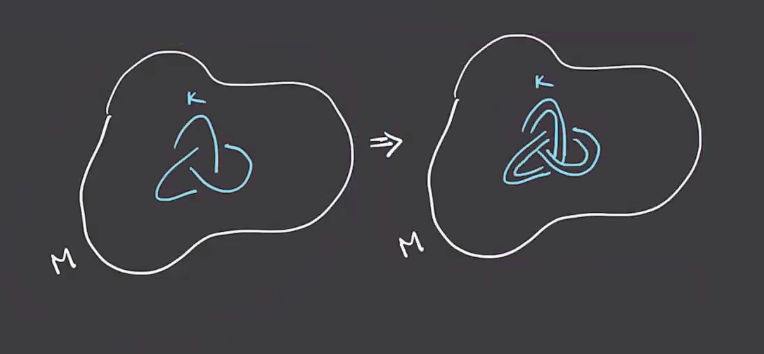
\includegraphics{figures/image_2021-01-19-12-23-16.png}
\caption{image\_2021-01-19-12-23-16}
\end{figure}

Taking a new solid torus \(S \coloneqq{\mathbb{D}}^2 \times S^1\) and a
diffeomorphism \(i: {{\partial}}S \to {{\partial}}(M \setminus N(K))\),
this yields a new manifold \(M _{\varphi} (K)\), a \textbf{surgery}
along \(K\).

\begin{figure}
\centering
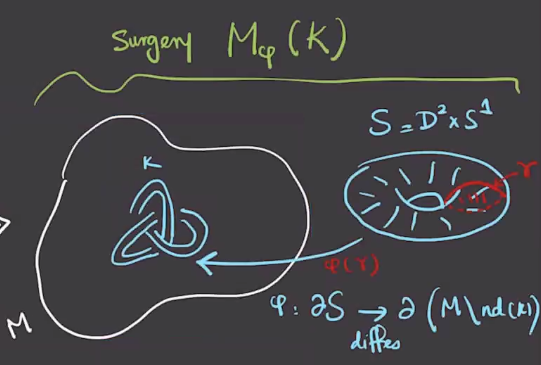
\includegraphics{figures/image_2021-01-19-12-25-25.png}
\caption{image\_2021-01-19-12-25-25}
\end{figure}

\end{definition}

\begin{remark}

Note that the diffeomorphism is entirely determined by the image of the
curve \(\alpha\) . The Knot Floer chain complex of \(K\) will allow us
to compute any flavor \(HF^{-}M _{\varphi} (K)\) of Floer homology. Why
is this important: any closed 3-manifold is surgery on a link in
\(S^3\). However there are many more computational tools available here
and not in the other theories: combinatorial approaches to compute,
exact sequences, bordered Floer homology.

\hfill\break

Next time: we'll talk about ``integer surgeries''.

\end{remark}

\hypertarget{lecture-3-morse-theory-thursday-january-19}{%
\section{Lecture 3: Morse Theory (Thursday, January
19)}\label{lecture-3-morse-theory-thursday-january-19}}

\hypertarget{intro-to-morse-theory}{%
\subsection{Intro to Morse Theory}\label{intro-to-morse-theory}}

\begin{remark}

Let \(M^n\) be a smooth closed manifold, then the goal is to study the
topology of \(M\) by studying smooth functions
\(f \in C^ \infty (M, {\mathbb{R}})\). We'll need \(f\) to be
\emph{generic} in a sense we'll discuss later.

\begin{figure}
\centering
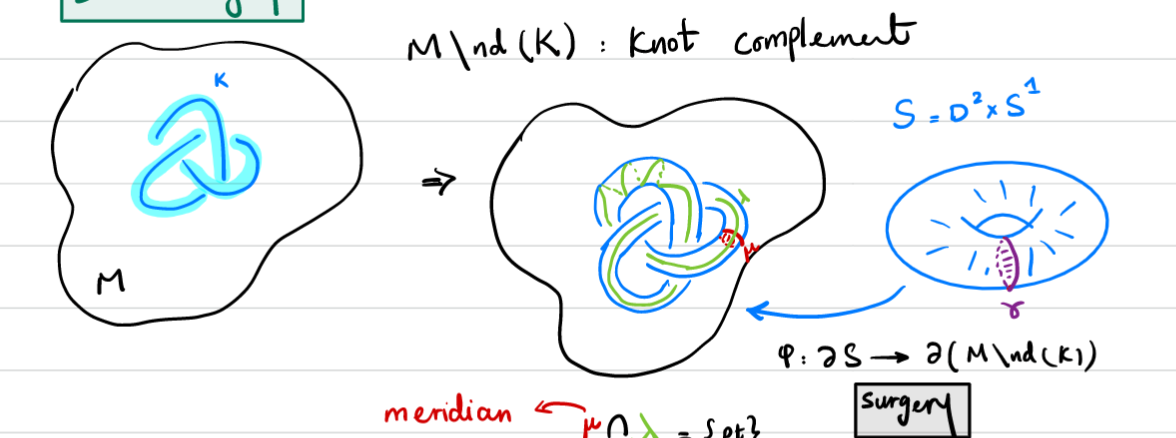
\includegraphics{figures/image_2021-01-19-00-41-55.png}
\caption{image\_2021-01-19-00-41-55}
\end{figure}

\end{remark}

\begin{definition}[Critical Point]

A point \(p\in M\) is called a \textbf{critical point} if and only if
\((df)_p = 0\).

\end{definition}

\begin{definition}[Hessian / Second Derivative]

Fixing a critical point \(p\) for \(f\), the \textbf{second derivative}
or \textbf{Hessian} of \(f\) at \(p\) is a bilinear form on \(T_pM\)
which is defined in the following way: for \(v, w\in T_p M\), extend
\(w\) to a vector field \(\tilde w\) in a neighborhood of \(p\) and set
\begin{align*}
d^2 f_p(v, w) = v\cdot (\tilde w \cdot f)(p) \coloneqq v \cdot (df)(\tilde w)(p)
.\end{align*}
where we take the derivative of \(f\) with respect to \(\tilde w\), then
take the derivative with respect to \(v\), then evaluate at the point to
get a number.

\end{definition}

\begin{remark}

This is only well-defined at critical points (check!). Note that we need
\(\tilde w\) so that \(\tilde w \cdot f\) is again a function (and not a
number) which can be differentiated again. You can also take
e.g.~\(\tilde v \cdot (\tilde w \cdot f)\), differentiating with respect
to the vector field instead of just the vector \(v\), but we're plugging
in \(p\) in either case.

\end{remark}

\begin{claim}

The second derivative is

\begin{enumerate}
\def\labelenumi{\arabic{enumi}.}
\item
  Well-defined, and
\item
  Symmetric
\end{enumerate}

\end{claim}

\begin{remark}

If you fix a coordinate chart in a neighborhood of \(p\), then the
bilinear form is represented by a matrix given by
\begin{align*}
(d^2 f)_p = H_p =  \qty{ {\frac{\partial ^2}{\partial x_j {\partial}x_i}\,}(p)}_{ij}
.\end{align*}

\end{remark}

\begin{proof}[of 2]

We can compute
\begin{align*}
(d^2 f)_p(v, w) - (d^2 f)_p(w, v) 
&= v\cdot (\tilde w \cdot f)(p) - w \cdot (\tilde v \cdot f)(p) \\
&\coloneqq df_p \qty{ [\tilde v, \tilde w]} \\
& = 0 && \text{since $p$ is a critical point and $df_p = 0$}
.\end{align*}

\end{proof}

\begin{proof}[of 1]

This is now easier to prove: we are picking an extension of \(w\) to a
vector field, so we need to show that the definition doesn't depend on
that choice.
\begin{align*}
(d^2 f)(_p(v, w) 
&= v\cdot (\tilde w \cdot f)(p) && \text{which doesn't depend on }\tilde v\\
&= (d^2 f)_p(w, v) \\
&= w\cdot (\tilde v \cdot f)(p) && \text{which doesn't depend on } \tilde w
,\end{align*}
and thus this is independent of both \(\tilde v\) and \(\tilde w\).

\end{proof}

\begin{exercise}[?]

Show that the second derivative in local coordinates is given by the
matrix \(H_p\) above.

\end{exercise}

\begin{remark}

In local coordinates, we can write
\(v = \sum_{i=1}^n a_i {\frac{\partial }{\partial x_i}\,}\) and
\(w = \sum_{i=1}^n b_i {\frac{\partial }{\partial x_i}\,}\), and thus
\begin{align*}
(d^2 f)_p(v, w) = \mathbf{b}^t H_p \mathbf{a} = \sum_{1 \leq i,j \leq n} a_i b_j {\frac{\partial ^2 f}{\partial x_i {\partial}x_j}\,}(p)
.\end{align*}

\end{remark}

\begin{definition}[Nondegenerate Critical Points]

A critical point \(p\in M\) is called \textbf{nondegenerate} if the
bilinear form \((d^2 f)_p\) is nondegenerate at \(p\), i.e.~for all
\(v\in T_p M\) there exists a
\(w\in T_pM\setminus\left\{{\mathbf{0}}\right\}\) such that
\((d^2 f)_p(v, w) \neq 0\). This occurs if and only if \(H_p\) is
invertible.

\end{definition}

\begin{definition}[Index of a critical point]

Given a nondegenerate critical point \(p\in M\), define the
\textbf{index} \(\operatorname{ind}(p)\) of \(f\) at \(p\) in the
following way: since \(H_p\) is symmetric and nondegenerate, its
eigenvalues are real and nonzero, so define the index as the number of
\emph{negative} eigenvalues of \(H_p\).

\end{definition}

\begin{definition}[Morse Function]

A function \(f\in C^ \infty (M, {\mathbb{R}})\) is called a
\textbf{Morse function} if and only if all of its critical points are
nondegenerate.

\end{definition}

\begin{remark}

We'll see that almost every smooth function is Morse, and these are
preferable since they have a simple and predictable structure near
critical points and don't do anything interesting elsewhere.

\end{remark}

\begin{theorem}[Morse Lemma]

Let \(p\in M\) be a nondegenerate critical point of \(f\) with
\(\operatorname{ind}(p) = \lambda\). Then there exists charts
\(\varphi:(U, p) \to ({\mathbb{R}}^n, 0)\) such that writing \(f\) in
local coordinates yields
\begin{align*}
(f \circ \varphi ^{-1} )(x) = f(p) - \sum_{i=1}^{\lambda} x_i^2 + \sum_{j= \lambda + 1}^n x_j^2
.\end{align*}

\end{theorem}

\begin{remark}[Observation 1]

We have
\begin{align*}
H_p = 
\begin{bmatrix}
-2&&&&&&\\
&\ddots&&&&&\\
&&-2&&&&\\
&&&2&&&\\
&&&&\ddots&&\\
&&&&&2&\\
&&&&&&2
\end{bmatrix}
= -2 I_{\lambda} \oplus 2 I_{n- \lambda}
.\end{align*}

\end{remark}

\begin{remark}[Observation 2]

If \(\lambda=n\)??

\end{remark}

\begin{remark}[Observation 3]

??

\end{remark}

\begin{example}[Sphere]

Consider \(S^2\) with a height function:

\begin{figure}
\centering
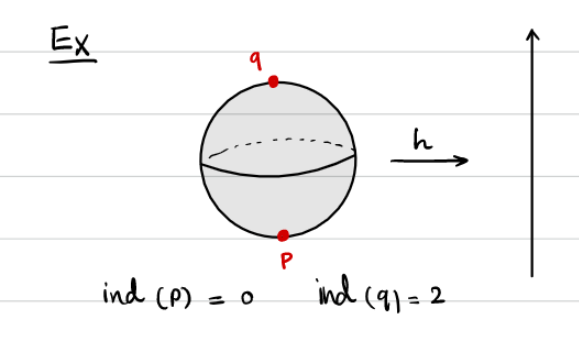
\includegraphics{figures/image_2021-01-19-00-49-32.png}
\caption{Sphere with a height function}
\end{figure}

Then we have a local minimum at the South pole \(p\) and a local max at
the North pole \(q\), where \(\operatorname{ind}(p) = 0\) and
\(\operatorname{ind}(q) = 2\). Note that the critical points essentially
occur where the tangent space is horizontal

\end{example}

\begin{example}[Torus]

Consider \({\mathbb{T}}^2\) with the height function:

\begin{figure}
\centering
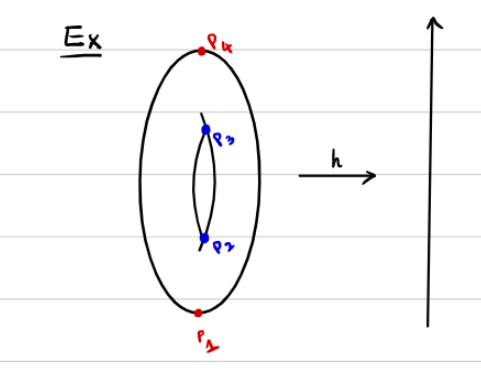
\includegraphics{figures/image_2021-01-19-00-49-53.png}
\caption{Torus with a height function}
\end{figure}

This has a similar max/min as the sphere, but also has two critical
points in the middle that resemble saddles:

\begin{figure}
\centering
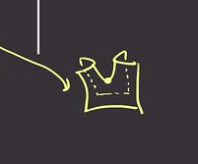
\includegraphics{figures/image_2021-01-21-12-04-50.png}
\caption{Saddle points}
\end{figure}

\end{example}

\begin{remark}

Define \(M_a \coloneqq f ^{-1} ((- \infty , a])\); we then want to
consider how \(M_a\) changes as \(a\) changes:

\begin{figure}
\centering
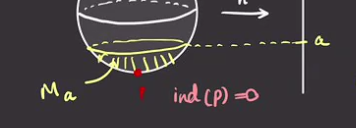
\includegraphics{figures/image_2021-01-21-12-06-29.png}
\caption{\(M_a\) on the sphere}
\end{figure}

\begin{figure}
\centering
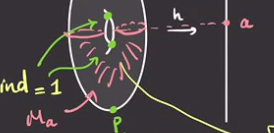
\includegraphics{figures/image_2021-01-21-12-06-49.png}
\caption{\(M_a\) on the torus}
\end{figure}

\end{remark}

\begin{lemma}[?]

If \(f ^{-1} ([a, b])\) contains no critical points, then
\begin{align*}
f ^{-1} (a) &\cong f ^{-1} (b) \\
M_a &\cong M_b
.\end{align*}

\end{lemma}

\begin{definition}[Gradients]

Choose a metric \(g\) on \(M\), then the \textbf{gradient vector} of
\(f\) is given by
\begin{align*}
g(\nabla f, v) = df(v)
.\end{align*}

\end{definition}

\begin{remark}

We have
\begin{align*}
df( \nabla f) = g(\nabla f, \nabla f) = {\left\lVert {\nabla f} \right\rVert}^2
.\end{align*}

\end{remark}

\begin{proof}[?]

We have the following situation:

\begin{figure}
\centering
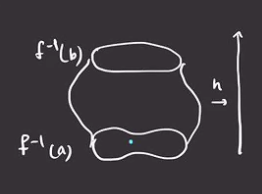
\includegraphics{figures/image_2021-01-21-12-11-16.png}
\caption{image\_2021-01-21-12-11-16}
\end{figure}

The gradient vector is always tangent to the level sets, so we can
consider the curve \(\gamma\) which satisfies
\(\dot\gamma(t) = -\nabla f( \gamma(t))\):

\begin{figure}
\centering
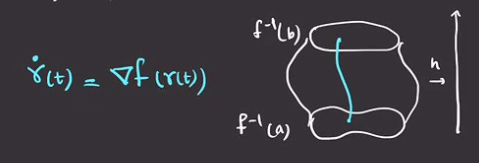
\includegraphics{figures/image_2021-01-21-12-12-42.png}
\caption{image\_2021-01-21-12-12-42}
\end{figure}

For technical reasons, we want to end up with cohomology instead of
homology and will take \(-\nabla f\) instead of \(\nabla f\) everywhere:

\begin{figure}
\centering
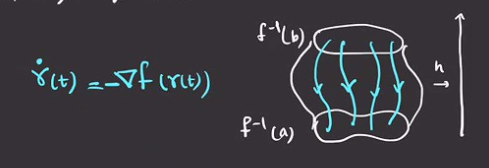
\includegraphics{figures/image_2021-01-21-12-13-35.png}
\caption{image\_2021-01-21-12-13-35}
\end{figure}

So \(\gamma\) will be a trajectory of \(- \nabla f\), and
\(f ^{-1} [a, b] \cong f ^{-1} (a) \times[0, 1]\). A problem is that
following these trajectories may involve arriving at \(f ^{-1} (a)\) at
different times:

\begin{figure}
\centering
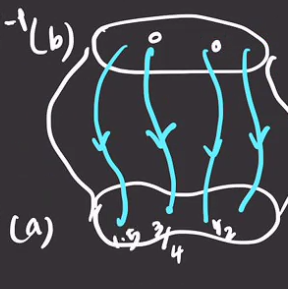
\includegraphics{figures/image_2021-01-21-12-15-10.png}
\caption{image\_2021-01-21-12-15-10}
\end{figure}

We can fix this by normalizing:
\begin{align*}
V \coloneqq- \nabla f / {\left\lVert { \nabla f} \right\rVert}^2 \implies (df)(v) = {\left\langle { \nabla f},~{ - \nabla f / {\left\lVert {\nabla f} \right\rVert}^2} \right\rangle} = -1
.\end{align*}

For every \(p \in f ^{-1} (b)\), if \(\gamma(t)\) is the trajectory
starting from \(p\), i.e.~\(\gamma(0) = p\), then
\(\gamma(b-a) \in f ^{-1} (a)\). So define
\begin{align*}
\Phi: f ^{-1} (b) \times[0, b-a] &\to f ^{-1} ([a, b]) \\
(p, t) &\mapsto \gamma_p (t)
,\end{align*}
which will be a diffeomorphism.

\end{proof}

\begin{theorem}[?]

Suppose \(f ^{-1} ([a, b])\) contains exactly one critical point \(p\)
with \(\operatorname{ind}(p) = \lambda\) and \(f(p) = c\). Then
\begin{align*}
M_b = M_a \cup_{{{\partial}}} \qty{ D^ \lambda \times D^{n - \lambda} }
\end{align*}
where \(n \coloneqq\dim M\).

\end{theorem}

\begin{example}[?]

For \(\lambda= 1, n - \lambda= 2\):

\begin{figure}
\centering
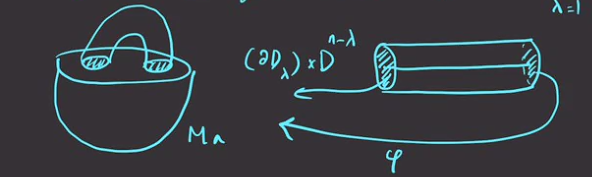
\includegraphics{figures/image_2021-01-21-12-32-38.png}
\caption{image\_2021-01-21-12-32-38}
\end{figure}

\end{example}

\begin{example}[?]

\begin{figure}
\centering
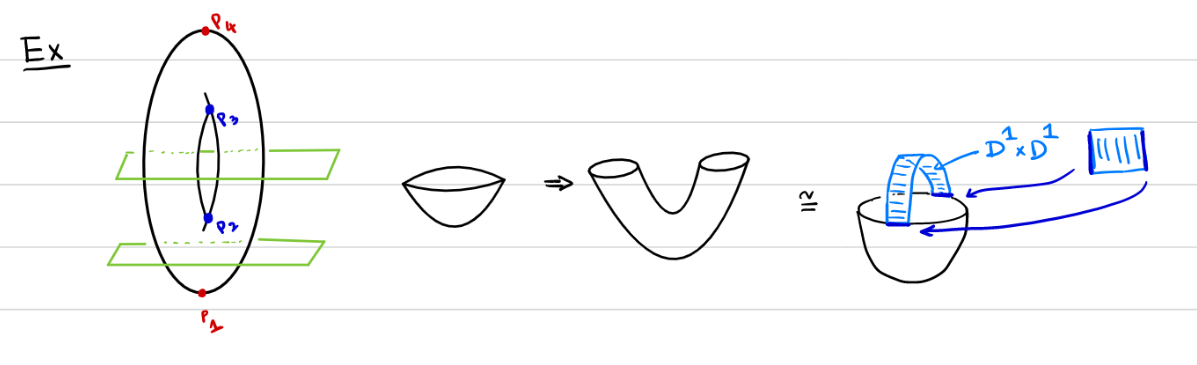
\includegraphics{figures/image_2021-01-19-00-53-07.png}
\caption{image\_2021-01-19-00-53-07}
\end{figure}

\end{example}

\begin{definition}[Unstable Submanifold]

\begin{align*}
W_f^u(p) \coloneqq\left\{{p}\right\} \cup\left\{{
\dot{\gamma(t)} = -\nabla f(\gamma(t)),\, \lim_{t\to -\infty} \gamma(t) = p,\, t\in {\mathbb{R}}
}\right\}
.\end{align*}

\end{definition}

\begin{lemma}[?]

If \(\operatorname{ind}(p) = \lambda\) then
\(W_f^u(p) \cong {\mathbb{R}}^ \lambda\).

\end{lemma}

\begin{example}[?]

\begin{figure}
\centering
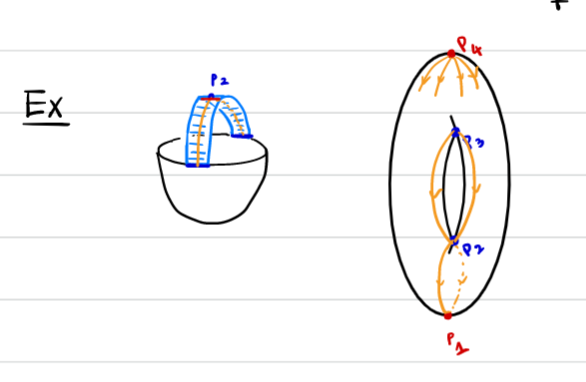
\includegraphics{figures/image_2021-01-19-00-55-24.png}
\caption{image\_2021-01-19-00-55-24}
\end{figure}

\end{example}

\begin{example}[?]

\begin{figure}
\centering
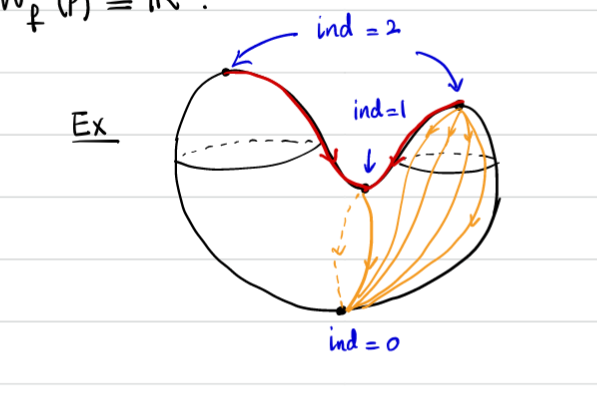
\includegraphics{figures/image_2021-01-19-00-55-41.png}
\caption{image\_2021-01-19-00-55-41}
\end{figure}

\end{example}

\begin{definition}[Stable Manifold]

\begin{align*}
W_f^s(p) \coloneqq\left\{{p}\right\} \cup\left\{{
\dot{\gamma(t)} = -\nabla f(\gamma(t)),\, \lim_{t\to +\infty} \gamma(t) = p,\, t\in {\mathbb{R}}
}\right\}
.\end{align*}

\end{definition}

\begin{lemma}[?]

If \(\operatorname{ind}(p) = \lambda\) then
\(W_f^s(p) \cong {\mathbb{R}}^{n- \lambda}\).

\end{lemma}

\begin{definition}[$C^\infty$ ]

\(C^ \infty (M; {\mathbb{R}})\) is defined as smooth function
\(M\to |RR\), topologized as:

\begin{itemize}
\tightlist
\item
  ?
\item
  ?
\end{itemize}

And a basis for open neighborhoods around \(p\) is given by
\begin{align*}
N_g(f) = \left\{{
g:M\to {\mathbb{R}}{~\mathrel{\Big|}~}
{\left\lvert {
{\frac{\partial ^k g}{\partial {\partial}x _{i_1} \cdots {\partial}x _{i_k} }\,}(p)
- 
{\frac{\partial ^k f}{\partial {\partial}x _{i_1} \cdots {\partial}x _{i_k} }\,}(p)
} \right\rvert} < \infty\, \forall \alpha,\, \forall p\in h_ \alpha(C_ \alpha)
}\right\}
.\end{align*}

\end{definition}

\begin{theorem}[?]

The set of Morse functions on \(M\) is open and dense in
\(C^ \infty (M; {\mathbb{R}})\).

\end{theorem}

\hypertarget{tuesday-january-26}{%
\section{Tuesday, January 26}\label{tuesday-january-26}}

\hypertarget{attaching-handles}{%
\subsection{Attaching Handles}\label{attaching-handles}}

\begin{remark}

Goal: we want to use Morse functions (smooth, nondegenerate critical
points) to study the topology of \(M\). Recall that the torus had 4
critical points,

\begin{figure}
\centering
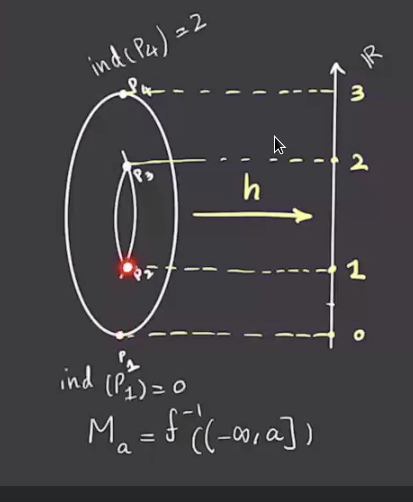
\includegraphics{figures/image_2021-01-26-11-14-32.png}
\caption{image\_2021-01-26-11-14-32}
\end{figure}

We defined the index as the number of negative eigenvalues of the
Hessian matrix. Here the highest index will be the dimension of the
manifold, and by the Morse lemma the two intermediate critical points
will be index 1.

\end{remark}

\begin{remark}

We want to use the Morse function to decompose the manifold, so we
consider \(M_a \coloneqq f ^{-1} ((- \infty , a ])\). If
\(f ^{-1} [a, b]\) does not contain a critical point, then
\(M_a \cong M_b\) and \(f ^{-1} (a) \cong f ^{-1} (b)\). So taking
\(M_{1/2}\) and \(M_{3/4}\) here both yield discs:

\begin{figure}
\centering
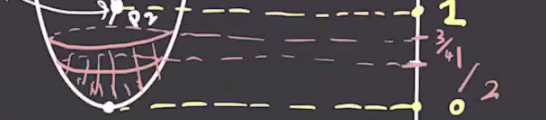
\includegraphics{figures/image_2021-01-26-11-17-46.png}
\caption{image\_2021-01-26-11-17-46}
\end{figure}

Passing through critical points does change the manifold, though:

\begin{figure}
\centering
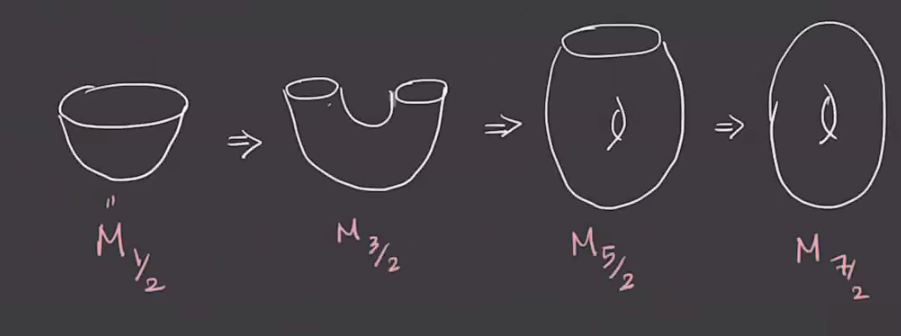
\includegraphics{figures/image_2021-01-26-11-19-01.png}
\caption{image\_2021-01-26-11-19-01}
\end{figure}

\end{remark}

\begin{theorem}[?]

Suppose \(f ^{-1} [a, b]\) contains exactly \emph{one} critical point of
index \(\lambda\) then
\begin{align*}
M_b \cong M_a \cup_{\varphi} (D_ \lambda \times D_{n - \lambda})
,\end{align*}
where
\(\varphi: ({{\partial}}D_ \lambda \times D_{ n - \lambda}) \hookrightarrow{{\partial}}M_a\).

\end{theorem}

\begin{example}[?]

For the case \(\lambda= 1, n = 3\), we have the following situation:

\begin{figure}
\centering
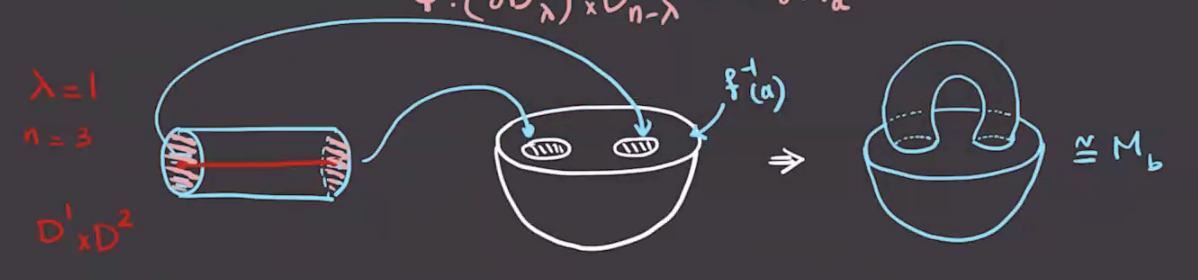
\includegraphics{figures/image_2021-01-26-11-24-46.png}
\caption{image\_2021-01-26-11-24-46}
\end{figure}

\end{example}

\begin{example}[?]

Taking \(\lambda=1, n=2\), we attach \(D^1 \times D^1\) and get the
following situation:

\begin{figure}
\centering
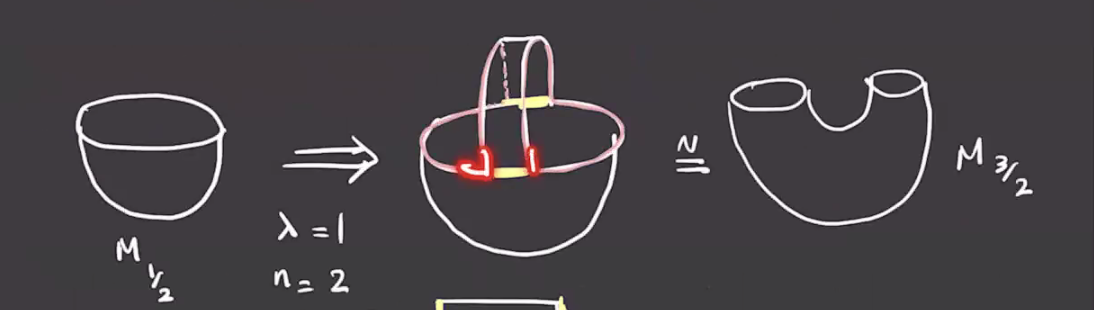
\includegraphics{figures/image_2021-01-26-11-27-16.png}
\caption{image\_2021-01-26-11-27-16}
\end{figure}

Adding on another piece, the new boundary is given by the highlighted
region:

\begin{figure}
\centering
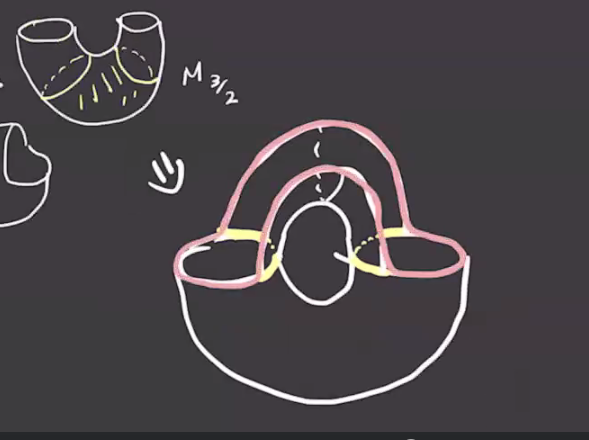
\includegraphics{figures/image_2021-01-26-11-32-27.png}
\caption{image\_2021-01-26-11-32-27}
\end{figure}

And continuing to attach the last pieces yields the following:

\begin{figure}
\centering
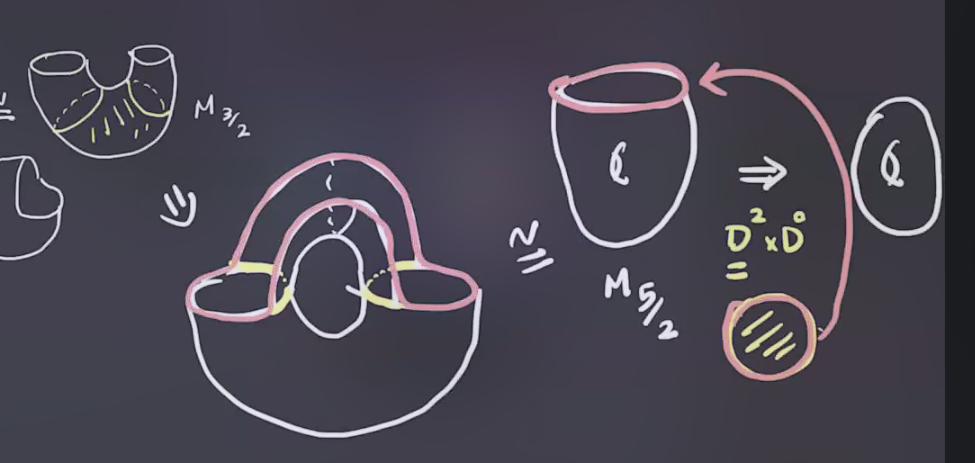
\includegraphics{figures/image_2021-01-26-11-33-31.png}
\caption{image\_2021-01-26-11-33-31}
\end{figure}

\end{example}

\begin{remark}

There is a deformation retract \(M_b \to M_a \cup C_ \lambda\), where
\(C_ \lambda\) is a \(\lambda{\hbox{-}}\)cell given by
\(D_ \lambda \times\left\{{0}\right\}\). For example:

\begin{figure}
\centering
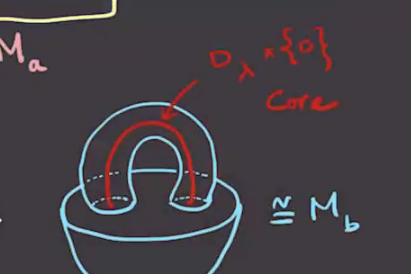
\includegraphics{figures/image_2021-01-26-11-36-35.png}
\caption{image\_2021-01-26-11-36-35}
\end{figure}

\end{remark}

\hypertarget{stable-and-unstable-manifolds}{%
\subsection{Stable and Unstable
Manifolds}\label{stable-and-unstable-manifolds}}

\begin{definition}[Unstable Manifold]

Given \(- \nabla f\) for a fixed metric, the \textbf{unstable manifold}
for a critical point \(p\) is defined as
\begin{align*}
W_f^u(p) \coloneqq\left\{{p}\right\} \cup\left\{{ \gamma(t) {~\mathrel{\Big|}~}\dot \gamma(t) = - \nabla f( \gamma(t) ),\, \gamma(t) \overset{t\to -\infty}\to p }\right\}
.\end{align*}
Here \(\gamma(t)\) is the trajectory of \(-\nabla(f)\).

\end{definition}

\begin{example}[?]

The unstable manifold is highlighted in blue here:

\begin{figure}
\centering
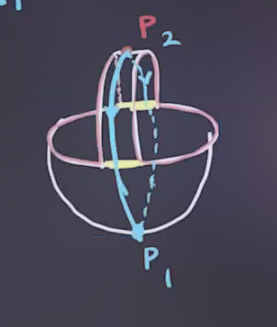
\includegraphics{figures/image_2021-01-26-11-42-01.png}
\caption{image\_2021-01-26-11-42-01}
\end{figure}

The gradient trajectories for other points are given by the yellow lines
in the following:

\begin{figure}
\centering
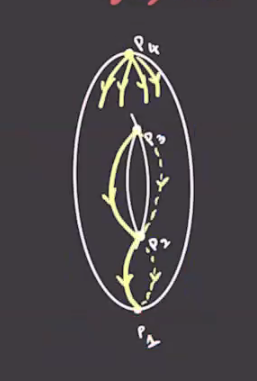
\includegraphics{figures/image_2021-01-26-11-44-13.png}
\caption{image\_2021-01-26-11-44-13}
\end{figure}

\end{example}

\begin{lemma}[?]

If \(\operatorname{ind}(p) = \lambda\), then the unstable manifold
\(W_f^u\) at \(p\) is isomorphic to \({\mathbb{R}}^ \lambda\).

\end{lemma}

\begin{example}[?]

\begin{figure}
\centering
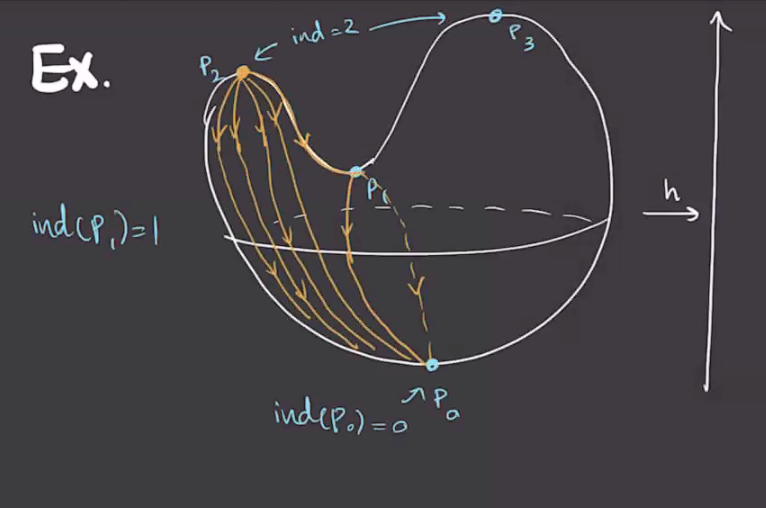
\includegraphics{figures/image_2021-01-26-11-46-46.png}
\caption{image\_2021-01-26-11-46-46}
\end{figure}

Here the unstable manifold for \(p_2\) will be 2-dimensional, with one
flow line ending at \(p_1\) and the rest ending at \(p_0\).

\begin{figure}
\centering
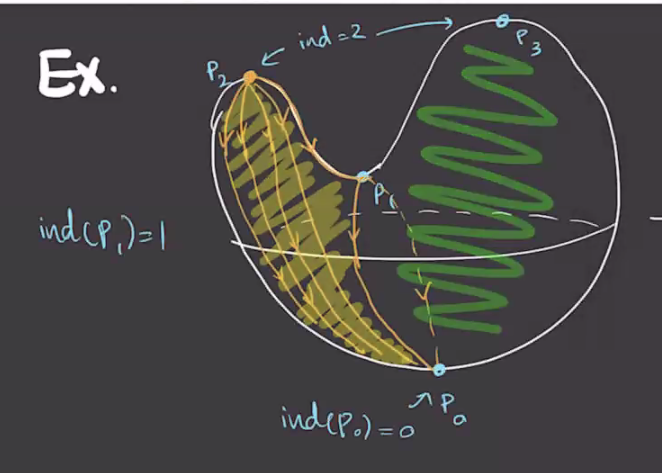
\includegraphics{figures/image_2021-01-26-11-47-24.png}
\caption{image\_2021-01-26-11-47-24}
\end{figure}

\end{example}

\begin{definition}[Stable Manifold]

The \textbf{stable manifold} for a critical point \(p\) is defined as
\begin{align*}
W_f^s(p) \coloneqq\left\{{p}\right\} \cup\left\{{ \gamma(t) {~\mathrel{\Big|}~}\dot \gamma(t) = - \nabla f( \gamma(t) ),\, \gamma(t) \overset{t\to {\color{red} +} \infty}\to p }\right\}
.\end{align*}

\end{definition}

\begin{example}[?]

The stable manifold for \(p_0\) above is every trajectory ending at
\(p_0\). \(W^s(p) = S^2 \setminus W^s(p_1) \cup W_s(p_3)\)? See video?

\todo[inline]{Which point $p$ is this for?}

\end{example}

\hypertarget{morse-functions}{%
\subsection{Morse Functions}\label{morse-functions}}

\begin{theorem}[Existence of Morse Functions]

The set of Morse functions is open and dense in
\(C^ \infty (M; {\mathbb{R}})\) in a certain topology.\footnote{See
  Akram's notes for details.}

\end{theorem}

\begin{remark}

We'll use this to define a chain complex \(C_*(f, g)\) where \(g\) is a
chosen metric, define a differential, and use this to define a homology
theory. For notation, we'll write \(\operatorname{crit}(f)\) as the set
of critical points of \(f\), and given
\(p, q\in \operatorname{crit}(f)\) with \(\gamma\) a trajectory running
from \(p\) to \(q\), we have
\begin{align*}
W^u(p) \cap W^s(q) = \left\{{ \gamma(t) {~\mathrel{\Big|}~}
\gamma(t) \overset{t\to -\infty }\to p,\,
\gamma(t) \overset{t\to +\infty }\to q
}\right\}
.\end{align*}

\end{remark}

\begin{definition}[Transverse Intersections]

Two submanifolds \(X, Y \subseteq M\) \textbf{intersect transversely} if
and only if
\begin{align*}
T_pX + T_p Y \coloneqq\left\{{v+w{~\mathrel{\Big|}~}v\in T_p X, w\in T_p Y}\right\} = T_p M && \forall p\in X \cap Y
.\end{align*}
In this case, we write \(X \pitchfork Y\).

\end{definition}

\begin{example}[?]

An example of a transverse intersection:

\begin{figure}
\centering
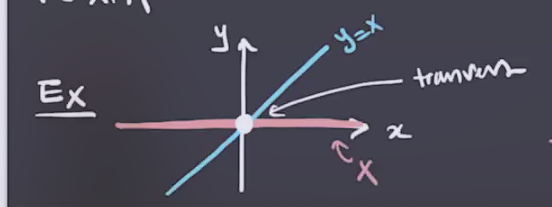
\includegraphics{figures/image_2021-01-26-12-02-29.png}
\caption{image\_2021-01-26-12-02-29}
\end{figure}

\end{example}

\begin{example}[?]

An example of an intersection that is \emph{not} transverse:

\begin{figure}
\centering
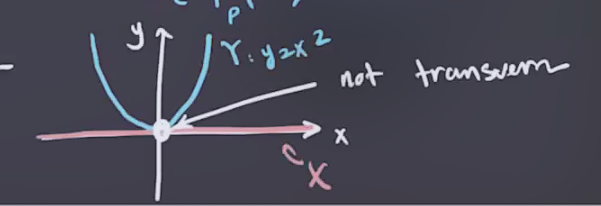
\includegraphics{figures/image_2021-01-26-12-03-13.png}
\caption{image\_2021-01-26-12-03-13}
\end{figure}

\end{example}

\begin{definition}[Morse-Smale]

A pair \((f, g)\) with \(f\) a Morse function and \(g\) a metric is
\textbf{Morse-Smale} if and only if

\begin{itemize}
\tightlist
\item
  \(f\) is a Morse function,
\item
  \(W^u(p)\) is \emph{transverse} to \(W^s(q)\) for all
  \(p, q\in \operatorname{crit}(f)\).
\end{itemize}

\end{definition}

\begin{theorem}[?]

For a generic metric \(g\), the pair \((f, g)\) is Morse-Smale.

\end{theorem}

\begin{remark}

This means that metrics can be perturbed to become Morse-Smale.

\end{remark}

\begin{example}[?]

The following is not Morse-Smale:

\begin{figure}
\centering
\includegraphics{figures/image_2021-01-26-12-06-06.png}
\caption{image\_2021-01-26-12-06-06}
\end{figure}

Note that if \(X^a \pitchfork Y^b\), then \(X \cap Y \subseteq M^n\) is
a smooth submanifold of dimension \(a+b-n\). In general, we have
\(M^s(p) \cong {\mathbb{R}}^{n - \lambda}\) where
\(\lambda = \operatorname{ind}(p)\).

\begin{observation}

If \((f, g)\) is Morse-Smale, then \(M^u(p) \pitchfork M^s(q)\). In this
case,
\begin{align*}
\dim(M^u(p) \cap M^s(q)) = \operatorname{ind}(p) + n - \operatorname{ind}(q) - n = \operatorname{ind}(p) - \operatorname{ind}(q)
.\end{align*}
Thus if \(\operatorname{ind}(p) = \operatorname{ind}(q)\) then
\(\dim M^s(p) \cap M^s(q) = 0\).

\end{observation}

\begin{remark}

There is an \({\mathbb{R}}{\hbox{-}}\)action of \(M^s(p) \cap M^s(q)\):
\begin{align*}
\qty{ M^s(p) \times M^u(q) } \times{\mathbb{R}}&\to M^s(p) \cap M^u(q) \\
( \gamma(t), c) &\mapsto \gamma(t+c)
.\end{align*}
If \(p\neq q\), this action is free and we can thus quotient by it to
obtain
\begin{align*}
\mathcal{M}(p, q) \coloneqq\qty{ M^s(p) \cap M^u(q)} / {\mathbb{R}}
.\end{align*}
This identifies all points on the same trajectory, yielding one point
for every trajectory, and so this is called the \textbf{moduli space of
trajectories from \(p\) to \(q\)}.

\end{remark}

If \(\operatorname{ind}(p) = \operatorname{ind}(q)\), we have
\(\dim M^u(p) \cap M^s (q) = 0\), making \(\dim \mathcal{M}(p, q) = -1\)
and thus \(\mathcal{M}(p, q) = \emptyset\) and no gradient trajectories
connect \(p\) to \(q\). Referring back to the example, since
\(\operatorname{ind}(p_3) = \operatorname{ind}(p_2)\), if \((f, g)\)
were Morse-Smale then there would be no trajectory \(p_3 \to p_2\),
whereas in this case there is at least one.

\end{example}

\begin{remark}

If \(\operatorname{ind}(p) - \operatorname{ind}(q) = 1\), then
\(\dim \mathcal{M}(p, q) = \operatorname{ind}(p) - \operatorname{ind}(q) - 1 = 0\),
making \(\mathcal{M}(p, q)\) a compact 0-dimensional manifold, which is
thus finitely many points, meaning there are only finitely many
trajectories connecting \(p\to q\) and it becomes possible to define a
Morse complex.

\end{remark}

\begin{definition}[Morse Complex]

Fix \((f, g)\) a Morse-Smale pair, then define
\begin{align*}
C_i(f, g) \coloneqq{\mathbb{Z}}/2{\mathbb{Z}}\left[\left\{{p {~\mathrel{\Big|}~}\operatorname{ind}p = i}\right\}\right] = \bigoplus_{\operatorname{ind}(p) = i} {\mathbb{Z}}/2{\mathbb{Z}}\left\langle{p}\right\rangle
,\end{align*}
with a differential
\begin{align*}
{{\partial}}: C_i(f, g) &\to C_{i-1}(f, g) \\
p, \operatorname{ind}(p) = i & \mapsto \sum_{\operatorname{ind}(q) = i-1} \# \mathcal{M}(p, q) q 
,\end{align*}
where we take the count mod 2.

\end{definition}

\begin{theorem}[?]

\({{\partial}}^2 = 0\), and thus \(( C(f, g), {{\partial}})\) is a chain
complex.

\end{theorem}

\begin{remark}

Next time we will work on proving this.

\end{remark}

\hypertarget{morse-homology-and-lagrangian-floer-homology-thursday-january-28}{%
\section{Morse Homology and Lagrangian Floer Homology (Thursday, January
28)}\label{morse-homology-and-lagrangian-floer-homology-thursday-january-28}}

\hypertarget{morse-homology}{%
\subsection{Morse Homology}\label{morse-homology}}

\begin{remark}

Last time: defined the Morse complex. Assumed \((f, g)\) was a
Morse-Smale pair, where \(f\) is a Morse function and \(g\) is a
Riemannian metric, and this guarantees that if
\(p, q\in \operatorname{crit}(f)\) with
\(\operatorname{ind}(p) - \operatorname{ind}(q) = 1\), then (among other
things) there are finitely many gradient trajectories \(p\leadsto q\).
We denoted this \(\mathcal{M}(p, q)\). The chain complex was defined by
\(C_i(f, g) \coloneqq\bigoplus_{\operatorname{ind}(p) = i} {\mathbb{Z}}_2 \left\langle{ p }\right\rangle\)
with differential \({{\partial}}_i: C_i \to C_{i-1}\) was defined by
sending an index \(i\) critical point \(p\) to
\(\sum_{\operatorname{ind}(q) = i-1} \# \mathcal{M}(p, q) q \pmod 2\).

\end{remark}

\begin{theorem}[The Morse Complex is a Chain Complex]

\({{\partial}}_{i} \circ {{\partial}}_{i+1} = 0\).

\end{theorem}

\begin{proof}[?]

Idea of the proof: we can directly compute
\begin{align*}
{{\partial}}({{\partial}}p) 
&= {{\partial}}\qty{ \sum_{\operatorname{ind}(q) = i-1} \# \mathcal{M}(p, q) q } \\
&= \sum_{\operatorname{ind}(q) = i-1} \# \mathcal{M}(p, q) {{\partial}}q \\
&= \sum_{\operatorname{ind}(q) = i-1} \# \mathcal{M}(p, q) \qty{ \sum_{\operatorname{ind}(r) = i-2 \# \mathcal{M}(q, r) r  }}   \\
&= \sum_{\operatorname{ind}(r) = i-2} \qty{\sum_{\operatorname{ind}(q) = i-1} \# \mathcal{M}(p, q) \# \mathcal{M}(q, r) }  r \\
&= \sum_{\operatorname{ind}(r) = i-2} c_{p,q,r} r \\
&= 0 && \text{(claim)}
.\end{align*}

This happens if and only if \(c_{p, q, r} = 0 \pmod 2\) for all \(r\)
with \(\operatorname{ind}(r) = i-2\). This is multiplication of the
number of trajectories:

\begin{figure}
\centering
\includegraphics{figures/image_2021-01-28-11-23-19.png}
\caption{image\_2021-01-28-11-23-19}
\end{figure}

In other words, this is the total number of trajectories \(p\leadsto r\)
that pass through \(q\). These trajectories ``break'' at \(q\), and so
we refer to these as \textbf{broken trajectories}.

\end{proof}

\begin{definition}[Broken Trajectories]

Suppose \(\operatorname{ind}(r) = \operatorname{ind}(p) - 2\), then a
\textbf{broken trajectory} from \(p\) to \(r\) is a trajectory from
\(p\) to \(q\) followed by a trajectory \(q\) to \(r\) where
\(\operatorname{ind}(q) = \operatorname{ind}(p)-1 = \operatorname{ind}(r) + 1\).

\begin{figure}
\centering
\includegraphics{figures/image_2021-01-28-11-26-25.png}
\caption{image\_2021-01-28-11-26-25}
\end{figure}

\end{definition}

\begin{question}

Why is the number of broken trajectories even?

\end{question}

\begin{answer}

We can check that
\(\dim \mathcal{M}(p, r) = \dim \qty{ W^u(p) \pitchfork W^s(r)}/{\mathbb{R}}= (\operatorname{ind}(p) - \operatorname{ind}(r)) - 1 = 2-1 = 1\).
We can compactify \(\mathcal{M}(p, r)\) by adding in all of the broken
trajectories to define
\begin{align*} 
\overline{\mathcal{M}(p, r)} \cup\qty{ \bigcup_{\operatorname{ind}(q) = i-1} \mathcal{M}(p, q) \times\mathcal{M}(q, r) } 
.\end{align*}
This is useful here because we can appeal to the classification of
smooth compact 1-dimensional manifolds, which are unions of copies of
\(S^1\) and \(D_1 = I\). In particular, the number of boundary points
\begin{align*}
{{\partial}}\overline{\mathcal{M}(p, r)} = \bigcup_{\operatorname{ind}(q) = i-1} \mathcal{M}(p, q) \times\mathcal{M}(q, r)
\end{align*}
is even:

\begin{figure}
\centering
\includegraphics{figures/image_2021-01-28-11-32-34.png}
\caption{image\_2021-01-28-11-32-34}
\end{figure}

\end{answer}

\begin{example}[Morse Homology of the Torus]

Suppose you have two critical points of the same index. The Morse-Smale
condition implies that there's no trajectory between them. A
counterexample would be \(p_3 \leadsto p_2\) on the torus with the
height function:

\begin{figure}
\centering
\includegraphics{figures/image_2021-01-28-11-45-16.png}
\caption{image\_2021-01-28-11-45-16}
\end{figure}

However, if you perturb this slightly, the trajectories can be made to
miss \(p_2\) and end at \(p_1\) instead. All of the trajectories are
disjoint, so we end up with a situation like the following after
perturbing the metric:

\begin{figure}
\centering
\includegraphics{figures/image_2021-01-28-11-48-06.png}
\caption{image\_2021-01-28-11-48-06}
\end{figure}

We can cut along a curve on the bottom to better analyze these
trajectories:

\includegraphics{figures/image_2021-01-28-11-48-57.png}
\includegraphics{figures/image_2021-01-28-11-50-27.png}

Now cut this cylinder along the trajectories
\(p_1\leadsto p_3 \leadsto p_1\), i.e.~the green trajectories here:

\begin{figure}
\centering
\includegraphics{figures/image_2021-01-28-11-51-31.png}
\caption{image\_2021-01-28-11-51-31}
\end{figure}

\begin{figure}
\centering
\includegraphics{figures/image_2021-01-28-11-53-32.png}
\caption{image\_2021-01-28-11-53-32}
\end{figure}

Here we can see that as the trajectories approach the corners, they
limit to broken trjacetories:

\begin{figure}
\centering
\includegraphics{figures/image_2021-01-28-11-54-44.png}
\caption{image\_2021-01-28-11-54-44}
\end{figure}

We can compute

\begin{itemize}
\tightlist
\item
  \(C_0 = {\mathbb{Z}}/2{\mathbb{Z}}\left\langle{ p_1 }\right\rangle\)
\item
  \(C_1 = {\mathbb{Z}}/2{\mathbb{Z}}\left\langle{ p_2, 3 }\right\rangle\)
\item
  \(C_2 = {\mathbb{Z}}/2{\mathbb{Z}}\left\langle{ p_4 }\right\rangle\)
\end{itemize}

Since there are exactly two trajectories \(p_4\) to \(p_2\) or \(p_3\),
we get \({{\partial}}_2 = 0\). Similarly \({{\partial}}_1 = 0\), and we
get
\(HM_i(T) = [{\mathbb{Z}}/2{\mathbb{Z}}, {\mathbb{Z}}/2{\mathbb{Z}}^2, {\mathbb{Z}}/2{\mathbb{Z}}, 0, \cdots]\),
which is the same as its singular homology.

\end{example}

\begin{theorem}[?]

\begin{align*}
HM_i(f, g) \cong H_i^{{\operatorname{Sing}}}(M; {\mathbb{Z}}/2{\mathbb{Z}})
.\end{align*}
In particular, it doesn't depend on the choice of Morse-Smale pair
\((f, g)\). See proof in references, e.g.~Audin.

\end{theorem}

\begin{proof}[?]

By definition,
\(\# \operatorname{crit}_i(f) = \operatorname{rank}C_i(f, g) = \operatorname{rank}HM_i(f, g)\),
and in any chain complex the rank of the chain groups are always at
least the rank of the homology.

\end{proof}

\hypertarget{lagrangian-floer-homology-1}{%
\subsection{Lagrangian Floer
Homology}\label{lagrangian-floer-homology-1}}

\begin{remark}

Suppose \(L_0^n, L_1^n \subset M^{2n}\) are compact with
\(L_0 \pitchfork L_1\), so the intersection is finitely many points.

\begin{figure}
\centering
\includegraphics{figures/image_2021-01-28-12-16-27.png}
\caption{image\_2021-01-28-12-16-27}
\end{figure}

We can do Morse theory on the space of paths between them:
\begin{align*}
\mathcal{P}(L_0, L_1) \coloneqq\left\{{ \gamma: I\to M {~\mathrel{\Big|}~}\gamma(0) \in L_0, \gamma(1) \in L_1}\right\}
.\end{align*}

We'll find analogs of Morse functions on \(P(L_0, L_1)\) such that the
critical points are constant paths, i.e.~\(L_0 \cap L_1\). The Morse
inequalities then gives bounds on the number of intersection points
between \(L_0\) and \(L_1\).

\end{remark}

\begin{definition}[Symplectic Manifolds]

A \textbf{symplectic manifold} is a pair \((M^{2n}, \omega)\) with
\(\omega\) a 2-form which is

\begin{itemize}
\tightlist
\item
  Closed, i.e.~\(d \omega = 0\), and
\item
  Nondegenerate, i.e.~\(\bigwedge^n \omega \neq 0\).
\end{itemize}

\end{definition}

\begin{definition}[Lagrangian Submanifolds]

A half-dimensional submanifold \(L^n \subset M^{2n}\) is called
\textbf{Lagrangian} if \({ \left.{{ \omega}} \right|_{{L^n}} } = 0\).

\end{definition}

\begin{example}[?]

The pair \(({\mathbb{R}}^{2n}, \sum_{i=1}^n dx_i \wedge dy_i\) is a
symplectic manifold (and also a symplectic vector space). Note that this
2-form is also a bilinear form of the following shape:

\begin{align*}
\begin{bmatrix}
0 & \operatorname{id}_n 
\\
-\operatorname{id}_n & 0
\end{bmatrix}
.\end{align*}

This has a Lagrangian submanifold
\({\mathbb{R}}^n \coloneqq\left\{{y_1 = \cdots = y_n = 0}\right\}\).

\begin{quote}
Note: See Darboux theorem.
\end{quote}

\end{example}

\begin{remark}

The general setup for next time: we'll have \((M^{2n}, \omega)\) a
symplectic manifold, a pair \(L_0, L_1 \subset M\) such that
\(L_0 \pitchfork L_1\), and we want to do Morse Homology on
\(\mathcal{P}(L_0, L_1)\).

\end{remark}

\hypertarget{lecture-6-tuesday-february-02}{%
\section{Lecture 6 (Tuesday, February
02)}\label{lecture-6-tuesday-february-02}}

\begin{remark}[Setup]

We're working with a symplectic manifold, i.e.~a pair
\((M^{2n}, \omega)\) where \(\omega \in \Omega^2\) is closed,
i.e.~\(d \omega = 0\), and nondegenerate,
i.e.~\(\bigvee^n \omega \neq 0\). We were also consider
\(L^n_0, L^n_1 \subset M\) Lagrangian submanifolds,
i.e.~\({ \left.{{ \omega }} \right|_{{L_i}} } = 0\). The goal is to do
something like Morse homology on \(\mathcal{P}(L_0, L_1)\) where the
critical points corresponds to intersection points \(L_0 \cap L_1\),
where we'll assume \(L_0 \pitchfork L_1\).

\end{remark}

\begin{question}

What is the analog of a Morse function?

\end{question}

\begin{remark}

The functional \(f\) is defined on the \emph{universal cover}
\(\overline{\mathcal{P}}(L_0, L_1) \to {\mathbb{R}}\). We can get around
knowing much about \(f\) because we only ever need derivatives \(df\)
and a metric \(g\) on the path space to talk about the gradient
\(\nabla_g f\). We'll define a 1-form
\(\alpha: T \mathcal{P}(L_0, L_1) \to {\mathbb{R}}\), where we can
define this tangent space as \(T_{\gamma} \mathcal{P}(L_0, L_1)\) where
\(\gamma(s): I \to M\). Set \(u(s, t)\) to be a path from \(\gamma\) to
\(\gamma'\) where \(u(s, 0) = \gamma\) and \(u(s, 1) = \gamma'\) and
\({\frac{\partial u}{\partial t}\,}\Big|_{t=0}\), which is a tangent
vector to \(\gamma\) and thus
\({\frac{\partial u}{\partial t}\,}(s, 0) \in T_{\gamma(s)}M\).

\begin{figure}
\centering
\includegraphics{figures/image_2021-02-02-11-29-54.png}
\caption{image\_2021-02-02-11-29-54}
\end{figure}

Upshot: tangent vectors in \(T_{\gamma} \mathcal{P}(L_0, L_1)\) are
given by \(\xi(s) \in T_{\gamma(s)}M\) for every \(s \in I\), i.e.~a way
to push the path off of itself to obtain a new path.

We can thus define
\begin{align*}
\alpha: T\mathcal{P}(L_0, L_1) &\to {\mathbb{R}}\\
( \gamma, \xi \in T_{\gamma} \mathcal{P}) &\mapsto \alpha_{\gamma}{\xi} \coloneqq\int_0^1 \omega( \dot{\gamma}(s), \xi(s)) ds
.\end{align*}
Does this have the property we want? I.e. is it zero when \(\gamma\) is
the constant path?

\end{remark}

\begin{lemma}[?]

\begin{align*}
\alpha _{\gamma} \equiv 0 \iff \gamma(s) \text{ is constant} \iff \dot{ \gamma(s)} = 0 \text{ for all } \gamma \iff \gamma(s) \in L_0 \cap L_1
.\end{align*}

\end{lemma}

\begin{proof}[?]

\begin{align*}
\alpha _{\gamma} \equiv 0 \iff \int_0^1 \omega( \dot{\gamma}(s), \xi(s)) ds = 0 \text{ for all } \xi\not\equiv 0
.\end{align*}

\begin{claim}

If \(\dot{\gamma}(s) \neq 0\) for some \(s\) then this is also true in
an open neighborhood by smoothness, so one can find a \(\xi\) such that

\begin{itemize}
\tightlist
\item
  \(\omega( \dot{\gamma(s)}, \xi(s) ) \geq 0\), and
\item
  There is some open subinterval \((a, b) \subseteq [0, 1]\) on which
  \(\xi\) is nonzero, and thus the integral is strictly positive.
\end{itemize}

\end{claim}

We'll need a few tools:

\begin{definition}[Almost Complex Structure]

An \textbf{almost complex structure} is a bundle automorphism
\(J: TM\to TM\) such that \(J \circ J = - \one_{TM}\). It is said to be
\textbf{compatible} with \(\omega\) if and only if

\begin{itemize}
\tightlist
\item
  Positivity: For every \(v\neq 0\), \(\omega(v, Jv) > 0\).
\item
  ``Symplectic Isometry'': For all \(v, w \in TM\),
  \(\omega(Jv, Jw) = \omega(v, w)\).
\end{itemize}

In this case, there is a Riemannian metric defined by
\(g(v, w) = \omega(v, Jw)\). Conversely, given an almost complex
structure \(J\) and a metric \(J\), there is a symplectic form defined
by \(\omega(v, w) = \omega(Jv, Jw) \coloneqq g(Jv, w)\).

\todo[inline]{This may not be a closed form? Need to check later!}

\end{definition}

\begin{exercise}[?]

Check that \(\omega\) is a symplectic form compatible with \(J\) and
\(g\) is the corresponding metric.

\end{exercise}

\begin{exercise}[?]

Given a symplectic form \(\omega\) and a Riemannian metric \(g\) there
exists a canonical almost complex structure \(J\) compatible with
\(\omega\) such that the previous process sends \((\omega, J)\) to
\(g\).

\end{exercise}

\begin{corollary}[?]

Any symplectic manifold \((M, \omega)\) has a compatible almost complex
structures \(J\).

\end{corollary}

\begin{theorem}[?]

The space of all almost complex structures on \(M\) compatible with
\(\omega\) is contractible.

\end{theorem}

Here we can use that \(\xi(s) = J \dot{ \gamma}(s)\) which implies
\(\omega( \dot{\gamma}(s), J \dot{\gamma(s)}) = \omega( \dot{ \gamma(s)}, \xi(s) ) > 0\),
which happens if and only if \(\dot{ \gamma}(s) \neq 0\).

So pick an almost complex structure compatible with \(\omega\) and
produce a metric \(g\). We'll define a metric on
\(\mathcal{P}(L_0, L_1)\) by the following: for
\(\xi, \eta \in T_{\gamma} \mathcal{P}\), recalling that
\(\xi = \xi(s), \eta = \eta(s) \in T_{\gamma(s)}M\), set
\begin{align*}
g_{\gamma}^\mathcal{P}( \xi, \eta) \coloneqq\int_0^1 g( \xi(s), \eta(s) ) ds = \int_0^1 \omega(\xi, J \eta) ds
.\end{align*}

\begin{exercise}[?]

Check that \(g^\mathcal{P}\) is a metric on \(\mathcal{P}(L_0, L_1)\).

\end{exercise}

We'll now define a \textbf{gradient vector field}:
\begin{align*}
g_{\gamma}^\mathcal{P}( -\nabla, {-}) = \alpha({-})
.\end{align*}
So here \(\alpha\) will play the role of \(-df\). We can write
\begin{align*}
\int_0^1 \omega( - \nabla, J \xi) ds = \int_0^1 \omega( \cdot{\gamma}, \xi) ds
.\end{align*}
Using compatibility, the LHS is equal to
\begin{align*}
\cdots = \int_0^1 \omega(-J \nabla, J^2 \xi) ds 
= \int_0^1 \omega(J \nabla, \xi) ds
.\end{align*}
So the RHS is equal to this for every \(\xi\), which means that
\(J \nabla= \dot{\gamma}\). Multiplying both sides by \(J\) yields
\(\nabla= -J \dot{\gamma}\) What are the trajectories of
\(J \cdot{ \gamma}(s)\in T_{\gamma} \mathcal{P}\)? We can compute
\begin{align*}
{\frac{\partial u}{\partial t}\,} (s, t) = J {\frac{\partial u}{\partial s}\,}(s, t)
.\end{align*}
Here \(t\) is the parameter that moves between paths, and \(s\) moves
along a given path:

\begin{figure}
\centering
\includegraphics{figures/image_2021-02-02-12-34-41.png}
\caption{image\_2021-02-02-12-34-41}
\end{figure}

\end{proof}

\hypertarget{lecture-7-thursday-february-04}{%
\section{Lecture 7 (Thursday February
04)}\label{lecture-7-thursday-february-04}}

\hypertarget{lagrangian-floer-homology-2}{%
\subsection{Lagrangian Floer
Homology}\label{lagrangian-floer-homology-2}}

\begin{remark}

Recall that we had a symplectic manifold \((M^{2n}, \omega)\) with
\(L_0, L_1 \subset M\) two Lagrangians. We wanted to do something like
Morse theory on \(\mathcal{P}(L_0, L_1)\).

\begin{figure}
\centering
\includegraphics{figures/image_2021-02-16-22-21-44.png}
\caption{image\_2021-02-16-22-21-44}
\end{figure}

What ingredients do we need?

\begin{itemize}
\item
  Something to replace \(-df\): \(\alpha\)
\item
  Something to replace the vector field \(-\nabla\): we defined a metric
  \(g^\mathcal{P}\) using \(\alpha\)
\end{itemize}

To define \(\alpha\) we needed to look at
\begin{align*}
T_{ \gamma} \mathcal{P}= \left\{{ \xi: I\to TM {~\mathrel{\Big|}~}\xi(s) \in T_{\gamma(s)}M }\right\} 
,\end{align*}
which is like a collection of tangent vectors along \(\gamma\) giving a
way to deform the path. Since \(\alpha\in \Omega^1(\mathcal{P})\), for
any \(\gamma\) it induces a map
\begin{align*}
T_{ \gamma} M &\xrightarrow{\alpha} {\mathbb{R}}\\
\xi &\mapsto \alpha_{ \gamma} (\xi) \coloneqq\int_0^1 \omega( \dot{ \gamma}, \xi)\,ds
.\end{align*}

\end{remark}

\begin{observation}

\(\alpha_{ \gamma} = 0 \iff \gamma\) is constant, which happens if and
only if \(\gamma\in L_0 \cap L_1\). This corresponds to critical points
of the functional yielding intersection points of the Lagrangians.

\end{observation}

\begin{remark}

We wanted to define the gradient, for which we needed a metric on
\(\mathcal{P}\). We did this by lifting a metric from \(M\). Pick an
almost complex structure \(J\) compatible with \(\omega\), then this
yields a Riemannian metric defined by \(g(v, w) = \omega(v, Jw)\). Then
we can define
\begin{align*}
g^\mathcal{P}_{\gamma}(\xi, \eta) \coloneqq\int_0^1 g( \xi(s), \eta(s) )\,ds
.\end{align*}
We used this to compute the vector field
\(-\operatorname{grad}_{\gamma} J \cdot{\gamma}(s)\). What are its
trajectories? These are paths of paths \(u(s, t) \coloneqq u_t(s)\) such
that
\({\frac{\partial }{\partial t}\,} u_t(s) = J {\frac{\partial }{\partial s}\,} u_t\).
We thus get an equation
\begin{align*}
{\frac{\partial u}{\partial t}\,}(s, t) = J {\frac{\partial u}{\partial s}\,}(s, t)
.\end{align*}

\end{remark}

\begin{remark}

For \(x, y \in L_0 \cap L_1\) trajectories connecting \(x\) to \(y\),
we'll write this as
\begin{align*}
\mathcal{M}(x, y) \coloneqq\left\{{ 
u(s, t) :[0,1] \times{\mathbb{R}}\to M 
\substack{ 
  u(0, t) \in L_0 \\ 
  u(1, t) \in L_1 \\ 
  u(s, t) \overset{t\to - \infty }\to x \\ 
  u(s, t) \overset{t\to \infty }\to y \\
  {\frac{\partial u}{\partial t}\,} = J {\frac{\partial u}{\partial s}\,}
} 
}\right\} 
.\end{align*}

We can modify this PDE to make things look familiar: multiply both sides
with \(J\) to obtain
\begin{align*}
J {\frac{\partial u}{\partial t}\,} = J^2 {\frac{\partial u}{\partial s}\,} \implies
J {\frac{\partial u}{\partial t}\,} = - {\frac{\partial u}{\partial s}\,} \implies
{\frac{\partial u}{\partial s}\,} + J {\frac{\partial u}{\partial t}\,} = 0
,\end{align*}
which is the Cauchy-Riemann equation.

\end{remark}

\begin{exercise}[?]

Check that this equation can be written as \(J\, du = du \circ i\) where
\(i\) is the standard complex structure on
\({\mathbb{C}}\supseteq [0, 1] \times{\mathbb{R}}\), so \(du\) commutes
with \(i\) and \(J\).

\end{exercise}

\begin{definition}[$J\dash$holomorphic or Pseudoholomorphic Discs]

If \(J\, du = du \circ i\), then \(u\) is called a
\textbf{\(J{\hbox{-}}\)holomorphic disc} or a \textbf{pseudoholomorphic
disc}.

\end{definition}

\begin{remark}

Schematically, the situation is the following:

\begin{figure}
\centering
\includegraphics{figures/image_2021-02-16-23-22-40.png}
\caption{image\_2021-02-16-23-22-40}
\end{figure}

Using the Riemann mapping theorem, the strip on the left-hand side is
biholomorphic to \({\mathbb{D}}\subseteq {\mathbb{C}}\) with \(\pm i\)
removed:

\begin{figure}
\centering
\includegraphics{figures/image_2021-02-16-23-23-43.png}
\caption{image\_2021-02-16-23-23-43}
\end{figure}

Due to the limit conditions at infinity in the strip, we can extend
\(u\) to a \(J{\hbox{-}}\)holomorphic map from the entire disc by
sending \(i\mapsto y\) and \(-i\mapsto x\).

\end{remark}

\begin{remark}

In Morse homology, we have an \({\mathbb{R}}\) action on the moduli
space of trajectories, and that also shows up here. Here
\({\mathbb{R}}\curvearrowright\mathcal{M}(x, y)\) by
\(u(s, t) \xrightarrow{c} u_c(s, t) \coloneqq u(s, t+c)\), noting that
translating the strip from above still yields a solution.

\end{remark}

\begin{definition}[?]

We define
\begin{align*}
\widehat{\mathcal{M}}(x, y) \coloneqq\mathcal{M}(x, y) / {\mathbb{R}}
.\end{align*}

\end{definition}

\begin{definition}[?]

We'll define
\begin{align*}
CF(L_1, L_2) \coloneqq\bigoplus_{x\in L_0 \cap L_1} {\mathbb{Z}}/2{\mathbb{Z}}\left\langle{ x }\right\rangle \\ \\
{{\partial}}x \coloneqq\sum_{y\in L_0 \cap L_1} \# \widehat{\mathcal{M}}(x, y) y 
.\end{align*}

\end{definition}

\begin{remark}

When is the intersection count \(\# \widehat{\mathcal{M}}(x, y)\)
well-defined? In Morse homology, we have two conditions:

\begin{enumerate}
\def\labelenumi{\arabic{enumi}.}
\item
  \((f, g)\) is Morse-Smale, to ensure that the moduli spaces are smooth
  manifolds (using Sard's theorem)
\item
  \(\operatorname{ind}(x) - \operatorname{ind}(y) = 1\), ensuring
  \(\mathcal{M}(x, y)\) is 1-dimensional
\item
  Compactness of \(\widehat{\mathcal{M}}(x, y)\) when 1 and 2 hold.
\end{enumerate}

These were enough to guarantee that \(\widehat{ \mathcal{M}} (x, y)\)
was a smooth compact 0-dimensional manifold, which allowed for point
counts. In Lagrangian Floer homology, we have the following
replacements:

\textbf{For 2 (indices)}: Recall that the index in Morse homology was
the dimension of the negative eigenspace of the Hessian, but we're in
infinite dimensions here. So we won't have a well-defined index, but
we'll have something that can replace the \emph{difference} of indices:
the \textbf{Maslov index} \(\mu(x, y)\), the expected dimension of
\(\mathcal{M}(x, y)\). To actually have this be the dimension will
require some conditions, so it's not always true. This will be the index
of some elliptic operator defined using the Cauchy-Riemann equations.

\textbf{For 1 (transversality)}: We'll need some version of
transversality, which will imply that for a generic \(J\) that
\(\mathcal{M}(x, y)\) is smooth.

\textbf{For 3 (compactness)}: We'll use \textbf{Gromov compactness} and
some extra topological assumptions, which will imply that
\(\widehat{ \mathcal{M}}(x, y), \mathcal{M}(x, y)\) are both compact.

Taken together, these will make the point-count well-defined.

\end{remark}

\begin{remark}

In order for this to be a chain complex, we'll need
\({{\partial}}^2 = 0\). We'll look at when \(\mu(x, y) = 2\), and we'll
compactify \(\widehat{ \mathcal{M}}(x, y)\) in order to show this holds.
Gromov's compactness will give us
\begin{align*}
{{\partial}}\overline{ \mathcal{M}(x, y) } = \bigcup_{\mu(x,z) = \mu(z, y) = 1} \mathcal{M}(x, z) \times\mathcal{M}(z, y) 
,\end{align*}
much like the \emph{broken trajectories} from Morse homology. Here we'll
need to add in broken \(J{\hbox{-}}\)holomorphic discs:

\begin{figure}
\centering
\includegraphics{figures/image_2021-02-16-23-45-04.png}
\caption{image\_2021-02-16-23-45-04}
\end{figure}

Using the same argument as in Morse homology, we can obtain
\({{\partial}}^2 = 0\).

\end{remark}

\begin{theorem}[Floer]

Suppose \((M^{2n}, \omega)\) is a compact symplectic manifold with
Lagrangians \(L_0, L_1\) such that

\begin{enumerate}
\def\labelenumi{\arabic{enumi}.}
\item
  \(L_0 \pitchfork L_1\)
\item
  \(\pi_2(M) = \pi_2(M, L_0) = \pi_2(M, L_1) = 0\), which are
  topological conditions on embedded spheres with boundaries mapped to
  the \(L_i\).
\end{enumerate}

Under these assumptions, \({{\partial}}^2 = 0\) and the homology
\begin{align*}
HF(L_0, L_1) \coloneqq H_*( CF(L_0, L_1), {{\partial}}) \coloneqq\ker {{\partial}}/ \operatorname{im}{{\partial}}
\end{align*}
is an invariant of \((M, L_0, L_1)\) up to \textbf{Hamiltonian
isotopies} of \(L_0, L_1\).

\end{theorem}

\begin{definition}[Symplectomorphism]

A \textbf{symplectomorphism} is a diffeomorphism \(\psi: M_1 \to M_2\)
such \(\psi^* \omega_1 = \omega_2\).

\end{definition}

\begin{definition}[Hamiltonian Vector Fields]

A \textbf{Hamiltonian vector field} is a vector field \(V\) such that
\begin{align*}
\iota_V \omega\coloneqq\omega(V, {-}) \in \Omega^1
\end{align*}
is exact, and thus equal to \(df\) for some functional
\(f\in C^{\infty }(M, {\mathbb{R}})\). Note that if one has a functional
\(f\), one can find a symplectic form \(\omega\) such that this holds,
so \(V\) is sometimes denoted \(V_f\) to show this dependence.

\end{definition}

\begin{example}[?]

\({\mathbb{R}}^{2n}\) with the standard symplectic form
\(\sum_{i=1}^n dx_i \wedge dy_i\), we have
\(V_f = {\frac{\partial f}{\partial y_1}\,}, \cdots, {\frac{\partial f}{\partial y_n}\,}, - {\frac{\partial f}{\partial x_1}\,}, \cdots, -{\frac{\partial f}{\partial x_n}\,}\)
for any \(f:{\mathbb{R}}^{2n} \to {\mathbb{R}}\). Note that we can have
time-dependent vector fields (i.e.~one parameter families) as well.

\end{example}

\begin{definition}[Hamiltonian Isotopies]

A \textbf{Hamiltonian isotopy} is a family \(\psi_t\) of diffeomorphisms
of \(M\) such that \(\psi_t\) is the flow of a 1-parameter family of
Hamiltonian vector fields \(V_t\), so taking the derivative of \(V\)
yields this function.

\end{definition}

\begin{exercise}[?]

Show that if \(\psi_t\) is a Hamiltonian isotopy, then
\(\psi_t^* \omega = \omega\) and is thus a symplectomorphism as well.

\end{exercise}

\begin{remark}

Goal: use this as an invariant of closed 3-manifolds in the form of
\textbf{Lagrangian Floer homology}, defined by Osvath-Szabo. Note that
Floer's theorem requires topological assumptions which make the homology
well-defined, but we don't have these available in the HF setup. In
particular, the assumptions on \(\pi_2\) won't hold.

\end{remark}

\hypertarget{lecture-8-thursday-february-04}{%
\section{Lecture 8 (Thursday, February
04)}\label{lecture-8-thursday-february-04}}

\hypertarget{heegard-splittings}{%
\subsection{Heegard Splittings}\label{heegard-splittings}}

\begin{remark}

Goal: we want to use \textbf{Lagrangian Floer homology} to defined
invariants of \emph{closed} 3-manifolds, where here closed means that
\({{\partial}}M^3 = \emptyset\). One example of Lagrangian Floer
homology is \textbf{Heegard Floer homology}. We'll want some symplectic
manifold with two Lagrangian submanifolds. Oszvath-Szabo used a
2-dimensional description of closed 3-manifolds called \textbf{Heegard
diagrams}. We'll need Heegard splittings to define these, and
handlebodies to define the splittings.

\end{remark}

\begin{definition}[Handlebody of genus $g$]

A \textbf{handlebody} of genus \(g\) will mean a compact 3-manifold
obtained from \({\mathbb{B}}^3\) by attaching \(g\) solid 1-handles,
i.e.~\({\mathbb{D}}^1 \times{\mathbb{D}}^2\). These are glued in via two
copies of \({{\partial}}{\mathbb{D}}^1 \times{\mathbb{D}}^2\):

\begin{figure}
\centering
\includegraphics{figures/image_2021-02-16-19-36-51.png}
\caption{image\_2021-02-16-19-36-51}
\end{figure}

Alternatively, these can be defined as a regular neighborhood of
\(\bigvee_{i=1}^g S^1 \subset {\mathbb{R}}^3\). We'll write \(H_g\) for
a genus \(g\) handlebody, and \({{\partial}}H_g\) will be a genus \(g\)
surface.

\end{definition}

\begin{definition}[Heegard Splitting]

A \textbf{Heegard splitting} of genus \(g\) is a decomposition
\(M = H_1 {\coprod}_{\varphi} H_2\) where
\(\varphi: {{\partial}}H_1 \to {{\partial}}H_2\) is a diffeomorphism.

\begin{figure}
\centering
\includegraphics{figures/image_2021-02-16-19-41-17.png}
\caption{image\_2021-02-16-19-41-17}
\end{figure}

Explicitly, we have
\begin{align*}
H_1 {\coprod}_{ \varphi} H_2 \coloneqq{ H_1 {\coprod}H_2 \over \left\langle{ x \sim \varphi(x) {~\mathrel{\Big|}~}\forall x \in {{\partial}}H_1 }\right\rangle }
.\end{align*}

\end{definition}

\begin{example}[?]

We can write \(S^3 = B_3 {\coprod}_{\one} B^3\), where both are just
genus \(0\) handlebodies. Note that if you attach a solid 1-handle to
\(B^3\), this yields \(S^1 \times{\mathbb{D}}^2\), i.e.~a solid torus:

\begin{figure}
\centering
\includegraphics{figures/image_2021-02-16-19-42-43.png}
\caption{image\_2021-02-16-19-42-43}
\end{figure}

Think of \(S^3\) as the one-point compactification of
\({\mathbb{R}}^3\), we can write (and visualize) a decomposition
\(S^3 = (S^1 \times{\mathbb{D}}^2) {\coprod}_{\varphi} (S^1 \times{\mathbb{D}}^2)\).
The first copy will be a neighborhood of a circle in the plane:

\begin{figure}
\centering
\includegraphics{figures/image_2021-02-16-19-44-16.png}
\caption{image\_2021-02-16-19-44-16}
\end{figure}

Labeling this circle as
\(H^1 \coloneqq\left\{{ x^2 + y^2 = 1, z = 0}\right\}\), the complement
\(H_2 \coloneqq S^3 \setminus H_1\) will be a regular neighborhood of
the \(z{\hbox{-}}\)axis union \(\left\{{\infty }\right\}\):

\begin{figure}
\centering
\includegraphics{figures/image_2021-02-16-19-45-36.png}
\caption{image\_2021-02-16-19-45-36}
\end{figure}

\end{example}

\begin{example}[?]

We can write a Heegard splitting of \(S^1 \times S^2\). Note that
\(S^2 = {\mathbb{D}}^2 {\coprod}_{\one} {\mathbb{D}}^2\), so splitting
the product over the union yields
\((S^1 \times{\mathbb{D}}^2) {\coprod}_{\one} (S^1 \times{\mathbb{D}}^2)\),
where the new map is still the identity since it's just the identity on
each factor. This yields two solid torii glued along their boundaries.

\end{example}

\begin{theorem}[?]

Any closed 3-manifold \(M^3\) admits a Heegard splitting.

\end{theorem}

\begin{proof}[?]

A fact from Morse theory: there exists a Morse function
\(f: M^3\to {\mathbb{R}}\) such that

\begin{enumerate}
\def\labelenumi{\arabic{enumi}.}
\item
  \(f(p) = i \coloneqq\operatorname{ind}(p)\) for every
  \(p\in \operatorname{Crit}(f)\) (i.e.~\(f\) is
  \textbf{self-indexing}), and
\item
  \(f\) has exactly one index \(0\) (minimum) and one index \(3\)
  (maximum) critical point.
\end{enumerate}

We thus have the following situation:

\begin{figure}
\centering
\includegraphics{figures/image_2021-02-16-19-51-11.png}
\caption{image\_2021-02-16-19-51-11}
\end{figure}

The remaining critical points must occur at 2 and 3:

\begin{figure}
\centering
\includegraphics{figures/image_2021-02-16-19-52-00.png}
\caption{image\_2021-02-16-19-52-00}
\end{figure}

How can we break this into smaller manifolds? Any time we pass a
critical point, we attach a one-handle. Note that we can define a new
Morse function \(h \coloneqq 3-f\) Suppose we have \(g\) critical points
of index 1 for \(f\) and \(g'\) critical points of index 1 for \(h\).

\begin{itemize}
\item
  We can check that \(f ^{-1} [0, 1/2] = {\mathbb{B}}^3\) and
  \(f ^{-1} (1/2) = S^2\).
\item
  \(f ^{-1} [0, 3/2] \Lambda_g,\) a genus \(g\) handlebody, and thus
  \(f ^{-1} (3/2) = \Sigma_g\) will be a genus \(g\) surface.

  \begin{figure}
  \centering
  \includegraphics{figures/image_2021-02-16-19-54-58.png}
  \caption{image\_2021-02-16-19-54-58}
  \end{figure}
\item
  Repeating the above arguments for \(h\), we get
  \(f ^{-1} [0, 3/2] = g ^{-1} [3/2, 3] = \Lambda_{g'}\).
\end{itemize}

\begin{exercise}[?]

Show that \(\operatorname{crit}(f) = \operatorname{crit}(h)\) and if
\(p\in \operatorname{crit}(f)\) with \(\operatorname{ind}_f(p) = i\)
then \(\operatorname{ind}_h(p) = 3-i\).

\end{exercise}

Thus \(g'\) is the number of index 2 critical points for \(f\). This
means that
\({{\partial}}h ^{-1} [0, 3/2] = h ^{-1} (3/2) = f ^{-1} (3/2)\) has
genus \(g=g'\), and thus the
\(\# \operatorname{crit}(f)_{\operatorname{ind}=1} = \# \operatorname{crit}(h)_{\operatorname{ind}=2} = g\).
Even without this, we still have our two handlebodies:
\(H_1 \coloneqq f ^{-1} [0, 3/2]\) and
\(H_2 \coloneqq f ^{-1} [3/2, 3]\) glued over
\(\Sigma_g \coloneqq f ^{-1} (3/2)\), which is a genus \(g\) splitting
surface.

\end{proof}

\begin{definition}[Equivalence of Heegard Splittings]

We'll say that two Heegard splittings
\(M = H_1 {\coprod}_{\varphi} H_2\) and
\(M = H_1' {\coprod}_{\varphi} H_2 '\) are \textbf{isotopic} if and only
if there exists an ambient isotopy \(\psi: M \times[0, 1] \to M\) such
that
\({ \left.{{\psi}} \right|_{{M \times\left\{{ 1}\right\} }} }(H_i) = H_i '\)
for each \(i\). Recall that \emph{ambient isotopy} means

\begin{itemize}
\item
  \({ \left.{{\psi}} \right|_{{ M \times\left\{{ 0 }\right\} }} } = \one\),
\item
  \({ \left.{{ \psi }} \right|_{{M \times\left\{{ t }\right\} }} }\) is
  a homeomorphism.
\end{itemize}

\end{definition}

\begin{question}

Are \emph{any} two Heegard splittings isotopic?

\end{question}

\begin{answer}

No! We can distinguish them by the genus of the splitting surface
\(\Sigma\), and we just saw two splittings of \(S^3\), one with genus 0
and one with genus 1.

\end{answer}

\begin{remark}

There are some moves to relate different Heegard splittings.

\end{remark}

\begin{definition}[Stabilization]

Given a genus \(g\) Heegard splitting
\(M = H_1 {\coprod}_{ \varphi} H_2\), we can produce a genus \(g+1\)
splitting \(M = H_1' \cup_{ \varphi} H_2'\) where

\(H_1' = H_1 \cup\overline{ \eta( \gamma) }\), where the new piece is a
closed regular neighborhood of an unknotted arc \(\gamma\) in \(H_2\).
Here \emph{unknotted} means that \(\gamma\) is a properly embedded arc
in \(H_2 \cup\Sigma\) whose boundary is in \(\Sigma\) which bounds a
contractible disc:

\begin{figure}
\centering
\includegraphics{figures/image_2021-02-16-21-00-33.png}
\caption{image\_2021-02-16-21-00-33}
\end{figure}

Note that adding a regular neighborhood around \(\gamma\) has the effect
of adding a 1-handle to \(H_1\). We can then define
\(H_2' \coloneqq H_2 \setminus\eta{\gamma}\). Why is this still a
handlebody? We have this situation:

\begin{figure}
\centering
\includegraphics{figures/image_2021-02-16-21-04-24.png}
\caption{image\_2021-02-16-21-04-24}
\end{figure}

We have the disc below the 1-handle, and if we thicken it to
\({\mathbb{D}}^2 \times I\), we have
\(B \coloneqq\eta(\gamma) \cup({\mathbb{D}}^2 \times[0, 1] \cong {\mathbb{B}}^3\):

\begin{figure}
\centering
\includegraphics{figures/image_2021-02-16-21-07-07.png}
\caption{image\_2021-02-16-21-07-07}
\end{figure}

We then have
\(H_2' \coloneqq(H_2 \setminus B) \cup({\mathbb{D}}^2 \cup[0, 1] )\),
and in fact there is something in the intersection of these two terms.
The parts that are attached to \(H_2\) are the front and back discs
\({\mathbb{D}}^2 \times\left\{{0, 1}\right\}\):

\begin{figure}
\centering
\includegraphics{figures/image_2021-02-16-21-07-50.png}
\caption{image\_2021-02-16-21-07-50}
\end{figure}

So we can identify this as
\(H_2' \coloneqq(H_2 \setminus B) {\coprod}_{{\mathbb{D}}^2 \times\left\{{ 0, 1 }\right\} } ({\mathbb{D}}^2 \cup[0, 1] )\).
Note that \(H_2 \setminus B \cong_{C^\infty} H_2\) are diffeomorphic,
and the right-hand side is a 1-handle. To see why this is, consider
attaching the middle red part, and then pushing the center part away in
order to see the handle:

\begin{figure}
\centering
\includegraphics{figures/image_2021-02-16-21-21-12.png}
\caption{image\_2021-02-16-21-21-12}
\end{figure}

\end{definition}

\begin{exercise}[?]

Show that the isotopy type of \(H_1' \cup H_2 '\) is independent of the
choice of \(\gamma\).

\end{exercise}

\begin{theorem}[?]

Any two Heegard splittings can be made isotopic after sufficiently many
stabilizations.

\end{theorem}

\hypertarget{heegard-diagrams}{%
\subsection{Heegard Diagrams}\label{heegard-diagrams}}

2-dimensional pictures of closed 3-manifolds! We have two handlebodies
glued along their boundary, so if we can write the handlebodies in terms
of 2-dimensional pictures, we can combine them to get a picture of the
entire splitting.

\begin{definition}[Attaching Curves]

Let \(H\) be a genus \(g\) handlebody. A set of \textbf{attaching
curves} for \(H\) is a set
\(\left\{{ \gamma_1, \cdots, \gamma_g }\right\}\) of pairwise disjoint
simple closed curves on \(\Sigma\coloneqq{{\partial}}H\) such that

\begin{enumerate}
\def\labelenumi{\arabic{enumi}.}
\item
  \(\Sigma\setminus\cup\left\{{\gamma_1, \cdots, \gamma_g}\right\}\) is
  connected,
\item
  All the \(\gamma_i\) bound a disc in \(H\).
\end{enumerate}

\end{definition}

\begin{example}[$S^1 \cross \DD^2$]

For the solid 2-torus, the attaching curves are copies of \(S^1\) that
bound discs

\begin{figure}
\centering
\includegraphics{figures/image_2021-02-16-21-27-56.png}
\caption{image\_2021-02-16-21-27-56}
\end{figure}

\end{example}

\begin{example}[A genus 2 handlebody]

Consider \({\mathbb{B}}^3\) with two 1-handles attached, or a solid
genus 2 surface:

\begin{figure}
\centering
\includegraphics{figures/image_2021-02-16-21-29-36.png}
\caption{image\_2021-02-16-21-29-36}
\end{figure}

Note that curves running around each of the two handles also work:

\begin{figure}
\centering
\includegraphics{figures/image_2021-02-16-21-30-26.png}
\caption{image\_2021-02-16-21-30-26}
\end{figure}

\end{example}

\begin{exercise}[?]

Show that
\(\Sigma\setminus\cup\left\{{ \gamma_1, \cdots, \gamma_g }\right\}\) is
connected \(\iff\) the classes \([\gamma_1], \cdots, [\gamma_g]\) are
linearly independent in \(H_1(\Sigma; {\mathbb{Z}})\).

\end{exercise}

\begin{proposition}[Handlebody from a Heegard Diagram]

Given a surface and a set of attaching curves, so the data of
\((\Sigma, \left\{{ \gamma_1, \cdots, \gamma_g }\right\} )\) , we can
build a handlebody \(H\). Note that we can go the other way: given a
genus \(g\) handlebody \(H\), we can take \(\Sigma = {{\partial}}H\) and
find \(g\) attaching circles.

\textbf{The recipe:}

\begin{enumerate}
\def\labelenumi{\arabic{enumi}.}
\item
  Thicken \(\Sigma\) to \(\Sigma \times[0, 1]\) to get a 3-manifold with
  2 boundary components, \(\Sigma\times\left\{{ 1 }\right\}\) and
  \(\Sigma \times\left\{{ 2 }\right\}\).
\item
  Attach thickened discs \(\gamma_i \times\left\{{ 0 }\right\}\) for
  each \(i\), yielding some \(S^2\) boundary components.
\item
  Fill the \(S^2\) boundary component with a \({\mathbb{B}}^3\).
\end{enumerate}

This yields a genus \(g\) handlebody \(H\) such that
\({{\partial}}H = \Sigma_g \times\left\{{ 1 }\right\}\), where the
curves
\(\left\{{ \gamma_1 \times\left\{{ 1 }\right\} , \cdots, \gamma_g \times\left\{{ 1 }\right\} }\right\}\).

\end{proposition}

\begin{example}[?]

Note that after attaching the disc on one end of this new cylinder, we
have the following:

\begin{figure}
\centering
\includegraphics{figures/image_2021-02-16-21-37-08.png}
\caption{image\_2021-02-16-21-37-08}
\end{figure}

What's left on the boundary is the following:

\begin{figure}
\centering
\includegraphics{figures/image_2021-02-16-21-37-43.png}
\caption{image\_2021-02-16-21-37-43}
\end{figure}

This is a copy of \(S^2\).

\end{example}

\begin{exercise}[?]

Show that for any \(g\) we get a 3-manifold with boundary
\(\Sigma \times\left\{{ 1 }\right\} {\coprod}S^2\) after step (2) above.

\end{exercise}

\hypertarget{lecture-9-thursday-february-11}{%
\section{Lecture 9 (Thursday, February
11)}\label{lecture-9-thursday-february-11}}

\hypertarget{heegard-diagrams-1}{%
\subsection{Heegard Diagrams}\label{heegard-diagrams-1}}

\begin{remark}

Last time we saw that \(M_3 = H_1 {\coprod}_{\varphi} H_2\) as two
handlebodies glued along their boundary by a diffeomorphism
\(\varphi: {{\partial}}H_1 \to {{\partial}}H_2\). This is referred to as
a \textbf{Heegard splitting} for \(M\). We can specify a genus \(g\)
handlebody as \(( \Sigma, \left\{{ \gamma_1, \cdots \gamma_g }\right\}\)
where \(\Sigma\setminus\left\{{ \gamma_1, \cdots, \gamma_g }\right\}\)
is connected and each \(\gamma_i\) bounds a disc in \(H\).

\begin{figure}
\centering
\includegraphics{figures/image_2021-02-11-11-15-56.png}
\caption{image\_2021-02-11-11-15-56}
\end{figure}

Moreover, we can go backwards: given such data, we can build a
handlebody \(H\) by

\begin{enumerate}
\def\labelenumi{\arabic{enumi}.}
\item
  Thickening \(\Sigma\) to obtain \(\Sigma \times[0, 1]\) This yields
  \({{\partial}}( \Sigma \times[0, 1] ) = (\Sigma\times\left\{{0}\right\} ) {\coprod}(\Sigma\times\left\{{1}\right\} )\).
\item
  Attach thickened discs to \(\gamma_i \times\left\{{0}\right\}\). This
  makes the boundary \((\Sigma \times\left\{{1}\right\} ) {\coprod}S_2\)
\item
  Fill in the \(S^2\) boundary with a \(B^3\).
\end{enumerate}

\begin{figure}
\centering
\includegraphics{figures/image_2021-02-11-11-22-43.png}
\caption{image\_2021-02-11-11-22-43}
\end{figure}

\end{remark}

\begin{definition}[Heegard Diagrams]

A \textbf{Heegard diagram} for \(M^3\) compatible with a splitting
\(M = H_1 {\coprod}_{ \varphi} H_2\) is a triple
\((\Sigma, \alpha, \beta\) where \(\alpha\) and \(\beta\) are attaching
circles for \(H_1\) and \(H_2\) respectively.

\end{definition}

\begin{example}[Heegard diagram for $S^3$]

The following two curves on a torus determine a Heegard splitting for
\(S^3\):

\begin{figure}
\centering
\includegraphics{figures/image_2021-02-11-11-28-43.png}
\caption{image\_2021-02-11-11-28-43}
\end{figure}

\end{example}

\begin{example}[Heegard diagram for $S^1 \cross S^2$]

Writing \(S^1 \times S^2 = D_2 {\coprod}_{\one_{{{\partial}}D^2}} D^2\),
or also \((S^1 \times D^2) {\coprod}_{\one} (S^1 \times D^2)\).

\begin{figure}
\centering
\includegraphics{figures/image_2021-02-11-11-30-50.png}
\caption{image\_2021-02-11-11-30-50}
\end{figure}

\end{example}

\begin{exercise}[?]

Show that the following diagram is a Heegard diagram for
\({\mathbb{RP}}^3\):

\begin{figure}
\centering
\includegraphics{figures/image_2021-02-11-11-31-45.png}
\caption{image\_2021-02-11-11-31-45}
\end{figure}

\emph{Hint: use that \({\mathbb{RP}}^3 \cong L(2, 1)\) and find a
Heegard diagram for \(L(p, q)\).}

\end{exercise}

\begin{example}[?]

Given a self-indexing Morse function \(f:M \to {\mathbb{R}}\) with
exactly one index 0 and one index 3 critical point, pick a generic
metric \(g\) so that \((f, g)\) is a Morse-Smale pair (so the stable and
unstable submanifolds intersect transversally). Taking \(- \nabla f\),
we can obtain a Heegard diagram The stable submanifolds are codimension
of their indices, so e.g.~for each index critical point there is a
2-dimensional stable submanifold that intersects the next submanifold in
a curve:

\begin{figure}
\centering
\includegraphics{figures/image_2021-02-11-11-36-23.png}
\caption{Stable submanifold}
\end{figure}

This occurs for (say) the \(g\) critical points of index \(1\) here, and
since they are distinct critical points the stable submanifolds are
disjoint. So we can obtain a set of attaching circles for the bottom
handlebody \(f ^{-1} ([0, 3/2])\):
\begin{align*}
\left\{{ M^s(p) \cap f ^{-1} (3/2) {~\mathrel{\Big|}~}p \in \operatorname{crit}(f),\, \operatorname{ind}(p) = 1 }\right\}
.\end{align*}

So setting these to be the \(\alpha\) curves, repeating with index 2 to
get \(\beta\) curves, and setting \(\Sigma\coloneqq f ^{-1} (3, 2)\) we
get a Heegard diagram for \(M\).

\end{example}

\begin{remark}

Note that given \((\Sigma, \alpha, \beta\) we can construct \(M\) in the
following way:

\begin{itemize}
\tightlist
\item
  \((\Sigma, \alpha\) builds \(H_ \alpha\) with
  \({{\partial}}H_{\alpha} = \Sigma\).
\item
  \((\Sigma, \beta\) builds \(H_ \beta\) with
  \({{\partial}}H_{\beta} = \Sigma\).
\end{itemize}

\end{remark}

\begin{exercise}[?]

Show that Heegard splittings can be used to compute homology, and
\begin{align*}
H_1(M; {\mathbb{Z}}) \cong H_1(\Sigma; {\mathbb{Z}}) / \left\langle{ [ \alpha_1] , \cdots, [ \alpha_g], [ \beta_1 ], \cdots, [\beta_g] }\right\rangle 
.\end{align*}

\end{exercise}

\hypertarget{heegard-moves}{%
\subsection{Heegard Moves}\label{heegard-moves}}

\begin{proposition}[?]

Given \(M = H_1 \cup H_2 = H_1' \cup H_2'\), we can \emph{stabilize} to
obtain \(M = \tilde H_1 \cup\tilde H_2\). Is there a way to relate the
two corresponding Heegard diagrams?

\begin{enumerate}
\def\labelenumi{\arabic{enumi}.}
\tightlist
\item
  Isotopy. Exchange
  \(\alpha = \left\{{ \alpha_1, \cdots, \alpha_g }\right\}\) with an
  ambient isotopy of \(\Sigma\), and similarly \(\beta\), keeping curves
  of the same type disjoint during the isotopy (where e.g.~it's fine if
  an \(\alpha\) curve intersects a \(\beta\) curve).
\end{enumerate}

\begin{figure}
\centering
\includegraphics{figures/image_2021-02-11-11-49-46.png}
\caption{image\_2021-02-11-11-49-46}
\end{figure}

\begin{enumerate}
\def\labelenumi{\arabic{enumi}.}
\setcounter{enumi}{1}
\tightlist
\item
  Handleslides (of \(\alpha\) or \(\beta\) curves).
\end{enumerate}

\begin{figure}
\centering
\includegraphics{figures/image_2021-02-11-11-51-54.png}
\caption{image\_2021-02-11-11-51-54}
\end{figure}

Equivalently, handle sliding \(\alpha_1\) over \(\alpha_2\) replaces
\(\alpha_1\) with \(\alpha_1'\) such that the triple
\(\alpha_1, \alpha_1', \alpha_2\) bound a pair of pants.

\begin{figure}
\centering
\includegraphics{figures/image_2021-02-11-11-53-22.png}
\caption{image\_2021-02-11-11-53-22}
\end{figure}

\begin{enumerate}
\def\labelenumi{\arabic{enumi}.}
\setcounter{enumi}{2}
\tightlist
\item
  Stabilization. This changes
  \((\Sigma, \alpha, \beta) \mapsto (\Sigma \mathop{ \Large\scalebox{0.8}{\raisebox{0.4ex}{\#}}}T^2, \alpha \cup\left\{{ \alpha_{g+1 } , \beta}\right\} \cup\left\{{ \beta_{g+1} }\right\}\),
  where \(\alpha_{g+1}, \beta_{g+1} \subseteq T^2\) and intersect in
  exactly on point.
\end{enumerate}

\begin{figure}
\centering
\includegraphics{figures/image_2021-02-11-12-10-06.png}
\caption{image\_2021-02-11-12-10-06}
\end{figure}

3'. Destabilization. Reversing the stabilization operation.

\end{proposition}

\begin{exercise}[?]

Show that any two sets of attaching curves for a handlebody \(H\) can be
related by a finite sequence of (1) and (2).

\end{exercise}

\begin{exercise}[?]

Show that stabilization yields a Heegard diagram for the same manifold.

\emph{Hint: the new summand is a Heegard diagram for \(S^3\), and
connect sums in the diagrams correspond to connect sums of the
corresponding manifolds. Moreover,
\(M \cong M\mathop{ \Large\scalebox{0.8}{\raisebox{0.4ex}{\#}}}S^3\).}

\end{exercise}

\begin{theorem}[?]

Any two Heegard diagrams for \(M\) can be connected by a finite sequence
of the above moves.

\end{theorem}

\hypertarget{tuesday-february-16}{%
\section{Tuesday, February 16}\label{tuesday-february-16}}

\begin{remark}

Note that critical points can be used to compute the Euler
characteristic, using the fact the \(\chi(C) = \chi(H_*(C))\), i.e.~it
can be computed on dimensions of chains or ranks of homology, along with
the fact that Morse homology is isomorphic to singular homology. So
e.g.~for a 3-manifold \(M^3\), we can show
\begin{align*}
\chi(M^3) 
&= \sum_{i=0}^3 {\operatorname{rank}}H_i \\
&= \sum_{i=0}^3 {\operatorname{rank}}CM_i \\
&= 1 - \# \operatorname{crit}_1(f) + \# \operatorname{crit}_2(f) - 1 \\
&= 0
,\end{align*}
since the number of index 2 and index 3 critical points will be the
same.

\end{remark}

\hypertarget{symmetric-product-spaces}{%
\subsection{Symmetric Product Spaces}\label{symmetric-product-spaces}}

\begin{remark}

Let \(M^3\) be a closed 3-manifold, then there is a Heegard splitting
\begin{align*}
(\Sigma_g, \alpha = \left\{{ \alpha_1, \cdots, \alpha_g }\right\}, \beta = \left\{{ \beta_1, \cdots, \beta_g }\right\} =( \Sigma_g, H_ \alpha, H_ \beta) && {{\partial}}(H_ \alpha) = {{\partial}}( H_ \beta) = \Sigma
,\end{align*}
where \(M^3 = H_{ \alpha} \coprod_{ \Sigma} H_ \beta\) and \(g\) is the
genus of \(HD\). We refer to \(\Sigma\) as a \textbf{Heegard surface},
and this set of data as a \textbf{Heegard diagram}.

We'll define \(\operatorname{Sym}^g( \Sigma)\) by letting
\(S_g \curvearrowright\Sigma^{\times g}\) where if \(\varphi\in S_g\) we
set
\(\varphi(x_1, \cdots, x_g) = x_{ \varphi(1)}, \cdots, x_{ \varphi(g) }\).
Then set \(\Sigma^{\times g} \coloneqq\Sigma^{\times g} / S_g\). Why
does this yield a smooth manifold? Is this action free? The diagonal
\(D \subseteq \Sigma^{\times g}\) consists of the points with at least 2
equal coordinates, and it's easy to see that \(S_g\curvearrowright D\)
can not be free. However, this still yields a smooth submanifold!

\end{remark}

\begin{lemma}[?]

\(\operatorname{Sym}^g(\Sigma)\) is smooth, and any complex structure
\(j\) on \(\Sigma\) will induce a complex structure on the quotient,
denoted \(\operatorname{Sym}^g(j)\), which is unique in the sense that
the quotient map
\(\Sigma^{\times g} \xrightarrow{\pi} \operatorname{Sym}^g(\Sigma)\) is
holomorphic.

\end{lemma}

\begin{proof}[?]

We'll check this locally, and then leave it as an exercise to check that
it extends globally -- this is easy by just considering what happens
under transition functions and checking that \(\pi\) is holomorphic.
Locally we want to produce a map
\begin{align*} 
\operatorname{Sym}^g({\mathbb{C}}) &\xrightarrow{f} {\mathbb{C}}^g \\
\left\{{ z_1, \cdots, z_g }\right\} &\mapsto \qty{ 
  \prod_{i=1}^g (z-z_i) 
  = z^g +a_1 z^{g-1} + \cdots + a_g \mapsto [a_1, \cdots, a_g] 
}
.\end{align*}
This is a bijection, and by the fundamental theorem of algebra, there is
an inverse. Equip \(\operatorname{Sym}^g({\mathbb{C}})\) with a complex
structure that makes \(f\) biholomorphic, then
\(\operatorname{Sym}^g(j)\) is the complex structure locally equal to
this one. This structure is obtained by just pulling back the standard
complex structure \(i\times i \times\cdots i\) on \({\mathbb{C}}^g\).

\end{proof}

\begin{remark}

\(\operatorname{Sym}^g( \Sigma)\) is a complex manifold of complex
dimension \(g\) (or real dimension \(2g\)). We want to find
half-dimensional submanifolds to do Lagrangian-Floer homology. Using the
Heegard splitting, write
\({\mathbb{T}}_ \alpha \coloneqq\prod_{i=1}^g \alpha_i \subset \Sigma^{\times g}\),
which is a \(g{\hbox{-}}\)dimensional torus such that
\({\mathbb{T}}_ \alpha \cap D = \emptyset\) since the \(\alpha_i\) are
pairwise disjoint. Composing the inclusion above with \(\pi\), we can
note that the action of \(S^g\) is free away from the diagonal \(D\), so
this composition is an embedding
\({\mathbb{T}}_ \alpha \hookrightarrow\operatorname{Sym}^g( \Sigma)\).
Similarly,
\({\mathbb{T}}_ \beta\coloneqq\prod_{i=1}^g \beta_i \hookrightarrow\operatorname{Sym}^g( \Sigma)\).

Note that we're only working with complex structures now, and haven't
upgraded it to a symplectic structure yet. But we don't really need this
to count holomorphic discs. Lagrangians \(L\) were defined as
submanifolds where \({ \left.{{\omega}} \right|_{{L}} } = 0\), how do we
do this without a symplectic form?

\end{remark}

\begin{definition}[?]

Given a complex manifold \((X, J)\), a submanifold \(L \subseteq X\) is
\textbf{totally real} if none of its tangent spaces contains a complex
line, i.e.~\(T_p L \cap J(T_p L) = \left\{{ p, \mathbf{0} }\right\}\)
for all \(p\in L\).

\end{definition}

\begin{example}[?]

Take a genus \(g\) surface \(\Sigma\):

\begin{figure}
\centering
\includegraphics{figures/image_2021-02-16-11-49-52.png}
\caption{image\_2021-02-16-11-49-52}
\end{figure}

Here any tangent vector has to get rotated out of the tangent space: if
it were an eigenvector for \(J\), then the rank of \(J\) would be too
low, contradicting its definition. Note that any 1-dimensional
submanifold of \((\Sigma, j )\) is totally real, and so
\({\mathbb{T}}_ \alpha, {\mathbb{T}}_ \beta\) are also totally real
submanifolds of \(\Sigma^{\times g}\). If you restrict \(\pi\) to
\(\Sigma^{\times g}\setminus D \xrightarrow{\pi} \operatorname{Sym}^g(\Sigma) \setminus\pi(D)\),
this yields a biholomorphic map.

\end{example}

\begin{remark}

We'll write
\(\Delta \coloneqq\pi(D) \subseteq \operatorname{Sym}^g( \Sigma)\). Note
that if \(\alpha\pitchfork\beta\), then
\({\mathbb{T}}_ \alpha \pitchfork{\mathbb{T}}_ \beta\). Any intersection
point \(x \in {\mathbb{T}}_{\alpha} \cap{\mathbb{T}}_{\beta}\) is of the
form \(x = \left\{{ x_1, \cdots, x_g}\right\} \subseteq \Sigma\) such
that each \(\alpha_i, \beta_j\) contain exactly one of the coordinates
of \(x\).

\end{remark}

\begin{example}[?]

The following is a diagram for \({\mathbb{RP}}^3\):

\begin{figure}
\centering
\includegraphics{figures/image_2021-02-16-12-00-55.png}
\caption{Heegard diagram for \({\mathbb{RP}}^3\)}
\end{figure}

Here \(g=1\) and so \(\operatorname{Sym}^1(T^2) = T^2\). We also have
\({\mathbb{T}}_{ \alpha} = \alpha, {\mathbb{T}}_{ \beta} = \beta\), and
their intersection is
\({\mathbb{T}}_{ \alpha} \cap{\mathbb{T}}_{ \beta} = \alpha \cap\beta = \left\{{A, B}\right\}\)

\end{example}

\begin{example}[Heegard diagram for the Poincaré homology sphere]

Here we have a Poincaré homology sphere \(P^3\), i.e.~a 3-manifold with
the same homology as \(S^3\),
i.e.~\(H_*(P^3) = [{\mathbb{Z}}, 0, 0, {\mathbb{Z}}]\) (??)

\begin{figure}
\centering
\includegraphics{figures/image_2021-02-16-12-01-57.png}
\caption{image\_2021-02-16-12-01-57}
\end{figure}

\begin{exercise}[?]

Compute \(H_*(P^3)\) using this diagram, particularly \(H_1\). Using
Poincaré duality here is fine!

\end{exercise}

The circles with the same color are the ``feet'' of a handle attachment,
or equivalently removing the two circles and identifying their boundary
with reversed orientation. The two different colors for circles indicate
that this will be genus 2 The arcs between same-colored circles indicate
loops that continue through the handle which aren't shown. Tracing
through the lines on the diagram, there are two \(\alpha\) curves and
two \(\beta\) curves. Since \(g=2\), we can identify
\(\operatorname{Sym}^2( \Sigma) \supseteq \alpha_1 \times\alpha_2 = {\mathbb{T}}_{\alpha}, \beta_1 \times\beta_2 = {\mathbb{T}}_{\beta}\).
The two black circles indicate intersection points in
\({\mathbb{T}}_{ \alpha} \cap{\mathbb{T}}_{ \beta}\). However, there are
more than just those two!

\begin{exercise}[?]

Show that
\({\left\lvert { {\mathbb{T}}_{ \alpha} \cap{\mathbb{T}}_{\beta} } \right\rvert} = 18\).

\end{exercise}

Computing the intersections:

\begin{center}
\begin{tikzcd}
    && {\beta_1} && {\beta_2} \\
    {\alpha_1} && 3 && 2 \\
    \\
    {\alpha_2} && 3 && 4
    \arrow["12"{description, pos=0.8}, dashed, tail reversed, from=2-3, to=4-5]
    \arrow["6"{description, pos=0.7}, dashed, tail reversed, from=4-3, to=2-5]
\end{tikzcd}
\end{center}

\todo[inline]{How to read this from the diagram?}

We're really working in \(\operatorname{Sym}^g(\Sigma)\), but for
computations, we'll work directly with the Heegard diagram.

\end{example}

\begin{remark}

For Lagrangian Floer homology, we'll have a triple
\((\operatorname{Sym}^g(\Sigma), {\mathbb{T}}_{ \alpha}, {\mathbb{T}}_{\beta} )\).
We'll define
\begin{align*}
CF( \Sigma, \alpha, \beta) \coloneqq\bigoplus_{x\in {\mathbb{T}}_{\alpha} \cap{\mathbb{T}}_{\beta} } {\mathbb{Z}}/2{\mathbb{Z}}\left\langle{ x }\right\rangle \\ \\
{{\partial}}(x) \coloneqq\sum_{y \in {\mathbb{T}}_{ \alpha} \cap{\mathbb{T}}_{\beta}, \mu = 1} \# \widehat{\mathcal{M}} y
.\end{align*}

We'll first figure out how to count continuous discs up to homotopy
classes, since holomorphic discs are much more restrictive. We'll see
that \(\pi_2\) plays a role, and define the topology of
\(\operatorname{Sym}^g\).

\end{remark}

\hypertarget{thursday-february-18}{%
\section{Thursday, February 18}\label{thursday-february-18}}

\begin{remark}

Today: topology of symmetric product spaces \(\operatorname{Sym}^g\). We
had an assignment
\begin{align*}
( \Sigma_g, \alpha, \beta) &\mapsto ( \operatorname{Sym}^g( \Sigma), {\mathbb{T}}_ \alpha, {\mathbb{T}}_ \beta)
,\end{align*}
where if \(\alpha, \beta\) are all transverse then so far
\({\mathbb{T}}_ \alpha, {\mathbb{T}}_ \beta\), since
e.g.~\({\mathbb{T}}_ \alpha = \prod_{i=1}^g \alpha_i\). We wanted to
define a chain complex
\begin{align*}
CF( \sigma, \alpha, \beta) \coloneqq\bigoplus _{x\in {\mathbb{T}}_ \alpha \cap{\mathbb{T}}_{ \beta } } {\mathbb{Z}}/2{\mathbb{Z}}\left\langle{ x }\right\rangle \\
{{\partial}}x \coloneqq\sum_{ \substack{ y \in {\mathbb{T}}_{ \alpha} \cap{\mathbb{T}}_{ \beta } \\  \mu(x, y)  = 1} } \# \mathcal{M}(x, y) y 
,\end{align*}
where \(\mu\) is the \emph{Maslov index} and we want to count
holomorphic discs. We'll first talk about continuous (topological)
discs.

\end{remark}

\begin{lemma}[?]

\begin{align*}
\pi_1( \operatorname{Sym}^g( \Sigma ) ) \cong H_1 ( \operatorname{Sym}^g( \Sigma ) ) \cong H_1 (\Sigma)
,\end{align*}
so the fundamental group is abelian.

\end{lemma}

\begin{remark}

For a proof of the first isomorphism, see Lemma 2.6 in
\autocite{OSZ04a}. Idea of proof for the second isomorphism: we'll
define a map
\begin{align*}
\iota: H_1 ( \Sigma) &\to H_1( \operatorname{Sym}^g( \Sigma) ) \\
x &\mapsto \left\{{ x, z, \cdots, z }\right\} 
,\end{align*}
for some fixed \(z \in \Sigma\), along with its inverse. Note that we're
identifying an embedding
\(\iota( \Sigma ) = \Sigma \times\left\{{ z }\right\}^{\times g-1} \subseteq \operatorname{Sym}^g( \Sigma)\).
Now define \(j \coloneqq\iota_*\) the induced map on homology.
\begin{align*}
j: H_1( \operatorname{Sym}^g (\Sigma) ) \to H_1 ( \Sigma) \\
.\end{align*}
Picking a loop \(\gamma: S^1 \to \operatorname{Sym}^g( \Sigma )\), note
that \(\Delta\subset \operatorname{Sym}^g( \Sigma)\) has codimension 2,
and so we can perturb \(\gamma\) to be disjoint from \(\Delta\). We can
arrange so that \(\gamma\) is the union of \(g\) paths
\(\gamma_1, \cdots, \gamma_g\) such that each \(\gamma_i\) connects
\(x_i \in \gamma(0)\) to \(x_{ \sigma(i) } \in \gamma(0)\) where
\(\gamma_0 = \left\{{ x_1, \cdots, x_g }\right\}\) and \(\sigma\in S_g\)
is a permutation.

\begin{example}[?]

For example, for \(g=3\):

\begin{figure}
\centering
\includegraphics{figures/image_2021-02-18-11-30-51.png}
\caption{image\_2021-02-18-11-30-51}
\end{figure}

Then \(\left\{{ \gamma_1(t), \gamma_2(t), \gamma_3(t) }\right\}\) is a
loop from \(\gamma(0) \to \gamma(0) \in \operatorname{Sym}^3( \Sigma)\).

\end{example}

This means that \(\bigcup_{i=1}^g \gamma_i\) is a 1-cycle in \(\Sigma\),
and thus \([ \cup g_i ] \in H_1( \Sigma)\). So we'll define this as
\(j([ \gamma ]) = [ \cup\gamma_i ]\).

Let
\(M \coloneqq\left\{{ (\mathbf{x}, y) {~\mathrel{\Big|}~}\mathbf{x} \in \operatorname{Sym}^g( \Sigma), y\in \mathbf{x} }\right\}\),
then we'll define a \(g:1\) branched cover away from
\(\pi ^{-1} \Delta\) that yields a fiber bundle:

\begin{center}
\begin{tikzcd}
    {S^1} && M \\
    \\
    {S^1} && {\operatorname{Sym}^g(\Sigma)} && \Sigma
    \arrow["{\exists \tilde \gamma}", dashed, from=1-1, to=1-3]
    \arrow["{\pi, \, g:1}", from=1-3, to=3-3]
    \arrow["{\exists g:1}"', dashed, from=1-1, to=3-1]
    \arrow["\gamma"', from=3-1, to=3-3]
    \arrow[curve={height=-18pt}, dotted, from=1-1, to=3-5]
    \arrow["{\pi_2}", curve={height=-24pt}, dotted, from=1-3, to=3-5]
\end{tikzcd}
\end{center}

\begin{quote}
\href{https://q.uiver.app/?q=WzAsNSxbMCwwLCJTXjEiXSxbMCwyLCJTXjEiXSxbMiwwLCJNIl0sWzIsMiwiXFxTeW0lZyhcXFNpZ21hKSJdLFs0LDIsIlxcU2lnbWEiXSxbMCwyLCJcXGV4aXN0cyBcXHRpbGRlIFxcZ2FtbWEiLDAseyJzdHlsZSI6eyJib2R5Ijp7Im5hbWUiOiJkYXNoZWQifX19XSxbMiwzLCJcXHBpLCBcXCwgZzoxIl0sWzAsMSwiXFxleGlzdHMgZzoxIiwyLHsic3R5bGUiOnsiYm9keSI6eyJuYW1lIjoiZGFzaGVkIn19fV0sWzEsMywiXFxnYW1tYSIsMl0sWzAsNCwiIiwwLHsiY3VydmUiOi0zLCJzdHlsZSI6eyJib2R5Ijp7Im5hbWUiOiJkb3R0ZWQifX19XSxbMiw0LCJcXHBpXzIiLDAseyJjdXJ2ZSI6LTQsInN0eWxlIjp7ImJvZHkiOnsibmFtZSI6ImRvdHRlZCJ9fX1dXQ==}{Link
to Diagram}
\end{quote}

This can be restricted to
\(M \setminus\pi ^{-1} (\Delta) \xrightarrow{g:1} \operatorname{Sym}^g( \Sigma) \setminus\Delta\).
Here \(j([ \gamma ]) = [ \pi_2 \circ \gamma]\) and
\(j \circ \iota_* = \one\).

\begin{example}[?]

We can use a Heegard diagram and Mayer Vietoris to compute the homology:
\begin{align*}
H_1( M; {\mathbb{Z}}) = 
{ 
H_1(\Sigma; {\mathbb{Z}}) 
\over 
\left\langle{ [\alpha_1], \cdots, [ \alpha_g], [\beta_1], \cdots, [\beta_g] }\right\rangle
}
\cong 
{ 
H_1( \operatorname{Sym}^g( \Sigma ) ) \over \left\langle{ H_1( {\mathbb{T}}_ \alpha ), H_1 ({\mathbb{T}}_ \beta ) }\right\rangle
}
.\end{align*}

\end{example}

\end{remark}

\begin{proposition}[?]

\begin{align*}
\pi_2( \operatorname{Sym}^g( \Sigma ) ) \cong {\mathbb{Z}}
.\end{align*}

\end{proposition}

\begin{remark}

The generator comes from hyperelliptic involution:

\begin{figure}
\centering
\includegraphics{figures/image_2021-02-18-11-58-40.png}
\caption{image\_2021-02-18-11-58-40}
\end{figure}

Then consider the quotient \(\Sigma / \tau\). To identify this quotient,
since the top half is identified with the bottom half, we can first
forget about the bottom half, and then forget about half of the arcs
along the axis of rotation:

\begin{figure}
\centering
\includegraphics{figures/image_2021-02-18-12-01-41.png}
\caption{image\_2021-02-18-12-01-41}
\end{figure}

Note that this results in a copy of \(S^2\). We can define a map
\begin{align*}
\Sigma &\to \Sigma^{\times g} \\
x &\mapsto (x, \tau(x), z, \cdots, z)
.\end{align*}
This extends to a map to \(\operatorname{Sym}^g( \Sigma)\), since
\(\tau(x) \mapsto (\tau(x), x, z, \cdots, z)\) and these will be equal
in \(\operatorname{Sym}^g\). So we can factor this through the quotient
from above:

\begin{center}
\begin{tikzcd}
    \Sigma &&& {\Sigma^{\times g}} \\
    \\
    {S^2} &&& {\operatorname{Sym}^g( \Sigma)}
    \arrow["f", from=1-1, to=1-4]
    \arrow["q"', from=1-1, to=3-1]
    \arrow[dashed, from=1-4, to=3-4]
    \arrow[dashed, from=3-1, to=3-4]
\end{tikzcd}
\end{center}

\end{remark}

\begin{definition}[Whitney Disc]

Given \(x, y \in {\mathbb{T}}_{ \alpha} \cap{\mathbb{T}}_{ \beta}\), a
\textbf{Whitney disc} from \(x\) to \(y\) is a map
\begin{align*}
\varphi: {\mathbb{D}}^2 \to \operatorname{Sym}^g( \Sigma) 
\end{align*}
such that
\begin{align*}
\phi(-i) &= x \\
\phi(i) &= y \\
\phi(e_1) &\subseteq {\mathbb{T}}_{ \alpha} \\
\phi(e_2) &\subseteq {\mathbb{T}}_{ \beta }
.\end{align*}

\begin{figure}
\centering
\includegraphics{figures/image_2021-02-18-12-22-03.png}
\caption{image\_2021-02-18-12-22-03}
\end{figure}

We say \(\varphi_1 \sim \varphi_2\) if and only if they are homotopic
relative to \({\mathbb{T}}_{ \alpha}, {\mathbb{T}}_{ \beta}\). We'll
write \(\pi_2(x, y)\) for the homotopy class of Whitney discs from \(x\)
to \(y\). There is a concatenation operation:
\begin{align*}
\ast: \pi_2(x, y) \times\pi_2(y, z) \to \pi_2(x, z)
.\end{align*}

\begin{figure}
\centering
\includegraphics{figures/image_2021-02-18-12-24-03.png}
\caption{image\_2021-02-18-12-24-03}
\end{figure}

Note that this is precisely concatenation of paths in the path space
\(\mathcal{P}\).

\end{definition}

\begin{exercise}[?]

If \(x=y=z\), then this yields an operation on \((\pi_2(x, x), \ast)\)
which defines a group.

\end{exercise}

\begin{remark}

We can find obstructions to holomorphic discs by just looking at the
topology. For
\(x, y\in {\mathbb{T}}_{ \alpha} \cap{\mathbb{T}}_{ \beta}\), choose two
paths connecting them:
\begin{align*}
a: I &\to {\mathbb{T}}_{ \alpha}\\
b: I &\to {\mathbb{T}}_{ \beta} 
.\end{align*}

\begin{figure}
\centering
\includegraphics{figures/image_2021-02-18-12-27-15.png}
\caption{image\_2021-02-18-12-27-15}
\end{figure}

We can consider the homology class \([a-b]\) to investigate \(\pi_1\).
This is well-defined as a loop
\begin{align*}
\varepsilon(x, y) \coloneqq[a-b] \in { H_1 ( \operatorname{Sym}^g ( \Sigma ) ) \over  \left\langle{ H_1( {\mathbb{T}}_{ \alpha } ) \oplus H_1 ( {\mathbb{T}}_{ \beta} ) }\right\rangle } \cong H_1(M)
.\end{align*}
This turns out to be independent of the choice of \(a, b\), and thus
\begin{align*}
\varepsilon(x, y) \neq 0 \implies \pi_2(x, y) = \emptyset
,\end{align*}
and there are no continuous discs.

\end{remark}

\hypertarget{tuesday-february-23}{%
\section{Tuesday, February 23}\label{tuesday-february-23}}

\hypertarget{whitney-discs}{%
\subsection{Whitney Discs}\label{whitney-discs}}

\begin{remark}

For \(x,y \in {\mathbb{T}}_{ \alpha} \cap{\mathbb{T}}_{ \beta}\), recall
that we had the following situation:

\begin{figure}
\centering
\includegraphics{figures/image_2021-02-23-11-14-22.png}
\caption{Whiteney Disc}
\end{figure}

Then \(\pi_2(x, y)\) was defined to be the homotopy classes of discs
connecting \(x\) to \(y\). The obstruction to the existence of such
discs was denoted \(\varepsilon(x, y) \in H_1(M)\) for
\(M\in {\mathsf{Mfd}}^3\). We're checking if there exist two paths
connecting \(x\) to \(y\),
\begin{align*}
a: I &\to {\mathbb{T}}_{ \alpha} \\
b: I &\to {\mathbb{T}}_{ \beta}
\end{align*}
such that \(a-b\) is nullhomotopic. In this case,
\(\pi_2(x, y) \neq \emptyset\).

\begin{figure}
\centering
\includegraphics{figures/image_2021-02-23-11-17-30.png}
\caption{image\_2021-02-23-11-17-30}
\end{figure}

We had a theorem that
\(\pi_1(\operatorname{Sym}^g \Sigma) \cong H_1( \operatorname{Sym}^g \Sigma)\),
so we can replace nullhomotopic with nullhomologous above. We can also
use the fact that
\(H_1( \operatorname{Sym}^g \Sigma) \cong H_1 \Sigma\). Note that
\([a-b]\) isn't well-defined, since we can append any loop to \(a\) for
example, but the following is well-defined:
\begin{align*}
\varepsilon(x, y) 
\coloneqq[a-b] \in { H_1 \operatorname{Sym}^g \Sigma \over H_1 {\mathbb{T}}_{ \alpha} \oplus H_1 {\mathbb{T}}_{ \beta} }
\cong {H_1 \Sigma \over \left\langle{ [ \alpha_1], \cdots, [ \beta_1 ], \cdots }\right\rangle} 
\cong H_1 M 
.\end{align*}

How can we compute \(\varepsilon\) using the Heegard diagrams? Recall
that a path in \(\operatorname{Sym}^g \Sigma\) was a union of \(g\)
paths in \(\Sigma\). So choose arcs \(a_1 \cup\cdots \cup a_g\) on
\(\Sigma\) such that \(a_i \subseteq \alpha_i\) is sub-arc and
\({{\partial}}( a_1 \cup\cdots \cup a_g ) = y_1 + \cdots + y_g - x_1 - \cdots - x_g\),
and similarly choose \(b_1 \cup\cdots \cup b_g\). Note that if
\(\varepsilon(x, y) \neq 0\) then \(\pi_2(x, y) = \emptyset\).

\end{remark}

\begin{example}[$L(2, 3)$]

The following is a Heegard diagram for \(L(2, 3)\) of minimal genus,
where we take \(\alpha\) to be the horizontal line and \(\beta\) will be
a line of slope \(2/3\):

\begin{figure}
\centering
\includegraphics{figures/image_2021-02-23-11-28-10.png}
\caption{image\_2021-02-23-11-28-10}
\end{figure}

Then
\({\mathbb{T}}_{ \alpha} \cap{\mathbb{T}}_{ \beta} = \left\{{ A, B }\right\}\).
Now draw arcs connecting \(A\) and \(B\), e.g.~the ones in orange and
green here:

\begin{figure}
\centering
\includegraphics{figures/image_2021-02-23-11-29-54.png}
\caption{image\_2021-02-23-11-29-54}
\end{figure}

Note that we have two generators of homology for the torus, say \(x,y\),
and we can write

\begin{figure}
\centering
\includegraphics{figures/image_2021-02-23-11-30-37.png}
\caption{image\_2021-02-23-11-30-37}
\end{figure}

Then the union of the two arcs is exactly \(x+y\), so we can write
\begin{align*}
H_1( L(2, 3)) 
= { {\mathbb{Z}}\left\langle{ x, y }\right\rangle \over \left\langle{ y, 2x + 3y }\right\rangle}  
.\end{align*}
Moreover, \(\varepsilon(A, B) = x + y \neq 0\) in this quotient, so
there is not Whitney disc connecting \(A\) to \(B\) and
\(\pi_2(A, B) = \emptyset\).

\end{example}

\begin{remark}

We'll define \(x\sim y \iff \varepsilon(x, y) = 0\), and this turns out
to be an equivalence relation which partitions the set of paths.

\begin{itemize}
\item
  \(\varepsilon(x, y) = 0 \implies \varepsilon(y, x) = 0\), which
  follows from \(\varepsilon(x, y) = [a-b] = [b-a] = \varepsilon(y, x)\)
\item
  \(\varepsilon(x, x) = 0\) by picking \(a,b\) constant.
\end{itemize}

\end{remark}

\begin{exercise}[?]

Show that \(\varepsilon(x, y) + \varepsilon(y, z) = \varepsilon(x, z)\).

\end{exercise}

\begin{corollary}[?]

If \(x\sim y\) and \(y\sim z\), so
\(\varepsilon(x, y) = \varepsilon(y, z) = 0\), we have
\(\varepsilon(x, z) = 0 \implies x \sim z\).

\end{corollary}

\begin{exercise}[?]

Find the equivalence classes under \(\sim\) for the Poincaré homology
sphere using the genus 2 Heegard diagram.

\end{exercise}

\begin{remark}

For \(\varphi\in \pi_2(x, y)\), the \textbf{shadow} is the 2-chain
\(D( \varphi )\) on \(\Sigma\) defined in the following way: remove the
\(\alpha, \beta\) arcs to obtain
\begin{align*}
\Sigma \setminus(\alpha\cup\sigma) = \displaystyle\coprod_{i=1}^m D_i
,\end{align*}

where \({}^{o}\) denotes that the set is open. Then
\(D( \varphi) = \sum_{i=1}^m a_i D_i\).

\end{remark}

\begin{definition}[?]

Given \(z\in \Sigma\setminus(\alpha\cup\beta)\), define a hyperplane
\begin{align*}
L_z = \left\{{ \mathbf{w} \in \operatorname{Sym}^g( \Sigma) {~\mathrel{\Big|}~}z\in \mathbf{w} }\right\} 
.\end{align*}
Note that this will be codimension 2. Then for a disc
\(\varphi\in \pi_2(x, y)\), define
\begin{align*}
n_z( \varphi ) = \# \qty{ \operatorname{im}( \varphi) \cap L_z }
.\end{align*}
which is an algebraic (signed) count of how many entries in a tuple
contain the point \(z\). We can then define
\(a_i \coloneqq n_{z_i}( \varphi)\) and define
\begin{align*}
D( \varphi) = \sum_{i=1}^m a_i D_i, && z_i \in {}^{o} D_i
.\end{align*}

\end{definition}

\begin{remark}

The following comes from ``Introduction to Heegard Floer Homology''
(Osvath-Szabo), which we've been following relatively closely so far.

\end{remark}

\begin{exercise}[?]

Let \(D\) be a domain of a disc connecting
\(\left\{{ x_1, x_2 }\right\}\) to \(\left\{{ y_1, y_2 }\right\}\) in
the following way:

\begin{figure}
\centering
\includegraphics{figures/image_2021-02-23-11-54-09.png}
\caption{image\_2021-02-23-11-54-09}
\end{figure}

Attach 1-handles in the following way to obtain \(\beta\) curves:

\begin{figure}
\centering
\includegraphics{figures/image_2021-02-23-11-55-13.png}
\caption{image\_2021-02-23-11-55-13}
\end{figure}

Use these handles to add curves running through the handles:

\begin{figure}
\centering
\includegraphics{figures/image_2021-02-23-11-56-26.png}
\caption{image\_2021-02-23-11-56-26}
\end{figure}

\begin{exercise}[?]

What is a Heegard diagram for?

\end{exercise}

Pick a point in the center of the rectangle and connect it to the 4
vertices, noting that it includes in \(\Sigma\) :

\begin{figure}
\centering
\includegraphics{figures/image_2021-02-23-11-58-15.png}
\caption{image\_2021-02-23-11-58-15}
\end{figure}

Applying a rotation by \(\pi\) and taking the quotient, we get a 2-fold
branched cover of \(S^1\):

\begin{figure}
\centering
\includegraphics{figures/image_2021-02-23-11-59-29.png}
\caption{image\_2021-02-23-11-59-29}
\end{figure}

Here \(x_1, x_2 \mapsto -i\) and \(y_1, y_2 \mapsto +i\). We can now get
a map \(\varphi\) to \(\operatorname{Sym}^2( \Sigma)\):

\begin{figure}
\centering
\includegraphics{figures/image_2021-02-23-12-01-02.png}
\caption{image\_2021-02-23-12-01-02}
\end{figure}

In the image we get 2 points with multiplicity on \(\Sigma\), and thus
an element of \(\operatorname{Sym}^2 \Sigma\). We know
\(\varphi(-i) = \left\{{ x_1, x_2 }\right\}\) and
\(\varphi(+i) = \left\{{ y_1, y_2 }\right\}\).

\end{exercise}

\begin{example}[?]

Show that \(D'\) is the domain of a disc from
\(\left\{{ x_1, x_2 }\right\} \to \left\{{ y_1, y_2 }\right\}\):

\begin{figure}
\centering
\includegraphics{figures/image_2021-02-23-12-18-15.png}
\caption{image\_2021-02-23-12-18-15}
\end{figure}

We want to make a similar 2-fold cover like in the previous example, so
we'll take the two rectangles bounding the arcs, then taking the
rotation by \(\pi\) yields the cover:

\begin{figure}
\centering
\includegraphics{figures/image_2021-02-23-12-20-27.png}
\caption{image\_2021-02-23-12-20-27}
\end{figure}

As before, we get a map to \(\operatorname{Sym}^2 \Sigma\):

\begin{figure}
\centering
\includegraphics{figures/image_2021-02-23-12-22-36.png}
\caption{image\_2021-02-23-12-22-36}
\end{figure}

As a result, we again get \(\varphi(-i) = \left\{{ x_1, x_2 }\right\}\)
and \(\varphi(+i) = \left\{{ y_1, y_2 }\right\}\).

\end{example}

\begin{exercise}[?]

. Suppose \(x = \left\{{ x_1, \cdots, x_g }\right\}\) and
\(y = \left\{{ y_1, \cdots, y_g }\right\}\) such that
\(x_i \in \alpha_i \cap\beta_i\) and
\(y_i \in \alpha_i \cap\beta_{ \sigma^{-1}(i)}\) for some permutation
\(\sigma\in S_g\). Then for any \(\varphi\in \pi_2(x, y)\), show that
\begin{align*}
  {{\partial}}\qty{{{\partial}}D( \varphi) \cap\alpha_i } = y_i - x_i
  ,\end{align*}
where the inner term is a 1-chain in \(\alpha_i\), and
\begin{align*}
  {{\partial}}\qty{ {{\partial}}D( \varphi) \cap\beta_i } = x_i - y_{ \sigma(i) }
  .\end{align*}

\end{exercise}

\begin{remark}

This will characterize the coefficients \(a_i\) for which discs exist.
Next time we'll talk about holomorphic discs.

\end{remark}

\hypertarget{thursday-february-25}{%
\section{Thursday, February 25}\label{thursday-february-25}}

\hypertarget{whitney-discs-1}{%
\subsection{Whitney Discs}\label{whitney-discs-1}}

\begin{remark}

Recall that we discussed the domains of discs: for
\(\varphi\in \varphi_2(x, y)\) we defined the 2-chain
\(D( \varphi) = \sum_{i=1}^n a_i D_i\) where we've written
\begin{align*} 
\Phi \setminus\alpha\cup\beta = {\coprod}_{i=1}^m \overset{\circ}{D_i} 
\end{align*}
and \(a_i\) is the number of points in
\(\operatorname{im}( \varphi) \cap L_{z_i}\) for \(z_i \in D_i\).

\end{remark}

\begin{exercise}[?]

For \(\varphi\in \pi_2(x, y)\), \({{\partial}}D( \varphi)\) is a 1-chain
in \(\alpha \cup\beta\). Then
\begin{align*} 
{ \left.{{ {{\partial}}D( \varphi )}} \right|_{{ \alpha}} } = \sum_{i=1}^g y_i - \sum_{i=1}^g x_i 
{ \left.{{ {{\partial}}D( \varphi )}} \right|_{{ \beta}} } = \sum_{i=1}^g x_i - \sum_{i=1}^g y_i 
\end{align*}
where \(x_i, y_i \in \alpha_i\).

\end{exercise}

\begin{corollary}[?]

For \(\varphi\in \pi_2(x, y)\), consider an intersection point \(w\)
which labels 4 nearby regions with coefficients \(a,b,c,d\):

\begin{figure}
\centering
\includegraphics{figures/image_2021-02-25-11-28-01.png}
\caption{image\_2021-02-25-11-28-01}
\end{figure}

Consider several cases:

\begin{enumerate}
\def\labelenumi{\arabic{enumi}.}
\item
  \(w\not\in x\) and \(w\not\in y\): Then
  \({{\partial}}\qty{ {{\partial}}{ \left.{{D( \varphi)}} \right|_{{ \alpha}} } } \not\ni w\).
  We can expand this out as
  \begin{align*}
    D( \varphi) = a D_1 + bD_2 + c D_3 + dD_4 \\
    {{\partial}}^2 D( \varphi) = {{\partial}}\qty{ a {{\partial}}D_1 } + {\cdots} 
    .\end{align*}
  Now restrict this to \(\alpha_i\) to yield
  \begin{align*}
    {{\partial}}^2 D( \varphi) = ae_1 + be_2 -ce_2 -de_1
    .\end{align*}
  Checking coefficients of \(w\) contributes \(-aw + bw - cw -d(-w)\),
  and these should sum to zero. This yields \(a+c = b+d\), and similarly
  if \(w\cap x \cap y\), this also yields \(a+c = b+d\).
\item
  \(w\in x\) and \(w\not \in y\) implies that \(a+c = b +d +1\).
\item
  \(w\not\in x\) and \(w\in y\) implies \(a+c+1 = b+d\).
\end{enumerate}

\end{corollary}

\begin{remark}

So if you want to check to see if some 2-chain could be the domain of a
Whitney disc, this local condition can be checked, i.e.~this is an
obstruction to existence. It turns out that this is an if and only if
condition.

\end{remark}

\begin{definition}[?]

A 2-chain \(A \coloneqq\sum_{i=1}^m a_i D_i\) \textbf{connects} \(x\) to
\(y\) if and only if the following local linear conditions are
satisfied:
\begin{align*}
{{\partial}}^2 { \left.{{A}} \right|_{{ \alpha}} } &= y-x \\
{{\partial}}^2 { \left.{{A}} \right|_{{ \beta}} } &= x-y \\
.\end{align*}

\end{definition}

\begin{proposition}[?]

Suppose \(g>1\). If a 2-chain \(A\) connects \(x\) to \(y\) then there
exists a Whitney disc \(\varphi\in \pi_2(x, y)\) such that
\(D( \varphi) = A\). If \(g>2\), \(\varphi\) is uniquely determined by
\(A\).

\end{proposition}

\begin{remark}

See proof in Osvath-Szabo paper.

\end{remark}

\begin{example}[?]

Think of the screen as a plane, and circled letters are handles attached
out of the page according to their orientations. Consider the following
diagram along with the indicated intersection points:

\begin{figure}
\centering
\includegraphics{figures/image_2021-02-25-11-45-11.png}
\caption{image\_2021-02-25-11-45-11}
\end{figure}

Set the coefficients of the unlabeled regions to zero, and let
\(x \coloneqq\left\{{ x_1, x_2}\right\}\) and
\(y \coloneqq\left\{{ y_1, y_2 }\right\}\). We can check that if the
following yellow region has coefficient 1, it can be the domain of a
Whitney disc:

\begin{figure}
\centering
\includegraphics{figures/image_2021-02-25-11-47-15.png}
\caption{image\_2021-02-25-11-47-15}
\end{figure}

This follows from checking the local conditions (there is a mnemonic
involving the diagonal sums for the various cases).

\end{example}

\begin{example}[?]

Consider a new diagram, changed by an isotopy (here: a ``finger move''):

\begin{figure}
\centering
\includegraphics{figures/image_2021-02-25-11-52-12.png}
\caption{image\_2021-02-25-11-52-12}
\end{figure}

Is there a Whitney disc connecting
\(x \coloneqq\left\{{ x_1, x_2 }\right\} \xrightarrow{\varphi} y \coloneqq\left\{{ y_1, y_2 }\right\}\)?
Checking the diagonals, all of the local conditions hold, so yes.

\end{example}

\begin{exercise}[?]

Find the 3-manifold that these two diagrams represent.

\end{exercise}

\hypertarget{holomorphic-discs}{%
\subsection{Holomorphic Discs}\label{holomorphic-discs}}

\begin{remark}

Ultimately these are what we want to define the differential in the
chain complex.

\begin{figure}
\centering
\includegraphics{figures/image_2021-02-25-12-08-55.png}
\caption{image\_2021-02-25-12-08-55}
\end{figure}

We'll set up a correspondence:
\begin{align*}
\left\{{\substack{
  (\text{Riemann surfaces } F, {\color{red} {{\partial}}_{ \alpha}}F, {\color{blue}{{\partial}}_{\beta}}F)
  \xrightarrow{\pi_{\Sigma}} ( \Sigma, {\color{red} \alpha}, {\color{blue} \beta }) \\
  {\big\Downarrow} \hspace{4em} {\scriptsize \text{$g{\hbox{-}}$fold branched cover $\pi_D$} } \\
  (D, e_1, e_2) \\
  {{\partial}}F = ({{\partial}}_{ \alpha} F) {\coprod}_{ {{\partial}}} ({{\partial}}_{ \beta} F) \\
  \pi_D( {{\partial}}_{ \alpha} ) = e_1 \hspace {2em}
  \pi_D( {{\partial}}_{ \beta} ) = e_2
}}\right\}
&\rightleftharpoons
\left\{{\substack{
\text{holomorphic }
u: (D^2, e_1, e_2) \to (\operatorname{Sym}^g(\Sigma), {\mathbb{T}}_{ \alpha}, {\mathbb{T}}_{ \beta})
  \text{}
}}\right\}
\end{align*}

To do this, we define
\(u(z) = \pi_{\Sigma}( \pi_D ^{-1}(z) ) \in \operatorname{Sym}^g(\Sigma)\).
Check that if \(\pi_D, \pi_\Sigma\) are holomorphic, then \(u\) is
holomorphic.

\begin{center}
\begin{tikzcd}
    &&& {} \\
    F && {\Sigma \times \operatorname{Sym}^{g-1}(\Sigma)} && \Sigma \\
    \\
    {D^2} && {\operatorname{Sym}^g(\Sigma)}
    \arrow["{g{\hbox{-}}\text{fold branched cover}}", from=2-3, to=4-3]
    \arrow["u"', from=4-1, to=4-3]
    \arrow["{\pi_D: g{\hbox{-}}\text{fold branched cover}}"', color={rgb,255:red,214;green,92;blue,92}, from=2-1, to=4-1]
    \arrow[color={rgb,255:red,214;green,92;blue,92}, from=2-1, to=2-3]
    \arrow["{\pi_1}"', from=2-3, to=2-5]
    \arrow["{\pi_\Sigma}"', curve={height=-24pt}, dashed, from=2-1, to=2-5]
\end{tikzcd}
\end{center}

\begin{quote}
\href{https://q.uiver.app/?q=WzAsNixbMCwzLCJEXjIiXSxbMiwzLCJcXFN5bV5nKFxcU2lnbWEpIl0sWzIsMSwiXFxTaWdtYSBcXHRpbWVzIFxcU3ltXntnLTF9KFxcU2lnbWEpIl0sWzAsMSwiRiJdLFs0LDEsIlxcU2lnbWEiXSxbMywwXSxbMiwxLCJnXFxkYXNoXFx0ZXh0e2ZvbGQgYnJhbmNoZWQgY292ZXJ9Il0sWzAsMSwidSIsMl0sWzMsMCwiXFxwaV9EOiBnXFxkYXNoXFx0ZXh0e2ZvbGQgYnJhbmNoZWQgY292ZXJ9IiwyLHsiY29sb3VyIjpbMCw2MCw2MF19LFswLDYwLDYwLDFdXSxbMywyLCIiLDAseyJjb2xvdXIiOlswLDYwLDYwXX1dLFsyLDQsIlxccGlfMSIsMl0sWzMsNCwiXFxwaV9cXFNpZ21hIiwyLHsiY3VydmUiOi00LCJzdHlsZSI6eyJib2R5Ijp7Im5hbWUiOiJkYXNoZWQifX19XV0=}{Link
to Diagram}
\end{quote}

Then if \(u\) is holomorphic, it can be shown that
\(\pi_D, \pi_{\Sigma}\) are also holomorphic. Given
\(\varphi\in \pi_2(x, y)\), define \(\mathcal{M}( \varphi)\) to be the
moduli space of holomorphic discs connecting \(x\) to \(y\) in the same
homotopy class as \(\varphi\) (i.e.~such discs \emph{represent}
\(\phi\)). After perturbing the complex structure
\(\operatorname{Sym}^g(j)\) to make it generic,
\(\mathcal{M}( \varphi)\) will be smooth. We'll have a notion of
dimension, the \emph{Maslov index} \(\mu( \varphi)\), which is the
expected dimension of \(\mathcal{M}( \varphi)\). There will be an
\({\mathbb{R}}{\hbox{-}}\)action on \(\mathcal{M}( \varphi)\), where we
remember the biholomorphism between the disc and the vertical strip:

\begin{figure}
\centering
\includegraphics{figures/image_2021-02-25-12-19-15.png}
\caption{image\_2021-02-25-12-19-15}
\end{figure}

We'll define
\(\widehat{ \mathcal{M}}( \varphi) \coloneqq\mathcal{M}( \varphi) / {\mathbb{R}}\).
The chain complex will be defined as
\begin{align*}
\operatorname{HF}( \Sigma, \alpha, \beta) &\coloneqq\bigoplus_{x \in {\mathbb{T}}_{ \alpha} \cap{\mathbb{T}}_{ \beta} } {\mathbb{Z}}/2 \left\langle{ x }\right\rangle 
\\
{{\partial}}x &\coloneqq\sum_{y\in {\mathbb{T}}_{ \alpha} \cap{\mathbb{T}}_{ \beta} } \sum _{ \varphi\in \pi_2(x, y) ?} \# \widehat{ \mathcal{M}}(\varphi)  
.\end{align*}

We'll need

\begin{itemize}
\item
  Check that \({{\partial}}\) is well-defined and \({{\partial}}^2=0\),
\item
  Check independence of choices, e.g.~the Heegard the diagram, the
  complex structure, the perturbations of \(\operatorname{Sym}^g(j)\),
  etc.
\end{itemize}

\end{remark}

\begin{question}

This takes a lot of work! Is the homology of this complex interesting?
Is this stronger than singular homology?

\end{question}

\begin{answer}

Let \(M \in \operatorname{ZHS}^3\), so the homology doesn't distinguish
\(M\) from a sphere and
\(H_*(M; {\mathbb{Z}}) \cong H_*(S^3; {\mathbb{Z}})\). It turns out that
\(H_*( \operatorname{HF}(M^3)) \cong H_*(\operatorname{HF}(S^3))\), so
the answer is no!

\end{answer}

\begin{remark}

Osvath-Szabo picked a basepoint
\(z\in \Sigma\setminus\qty{ \alpha\cup\beta}\) and work with
\emph{pointed} Heegard diagrams \((\Sigma, \alpha, \beta, z)\). Perturb
the differential to obtain
\begin{align*}
\tilde {{\partial}}x \coloneqq\sum_{y \in {\mathbb{T}}_{ \alpha} \cap{\mathbb{T}}_{ \beta} } 
\sum_{ \substack{ 
\varphi \in \pi_2(x, y), \\
\mu( \varphi) = 0, \\
n_z( \varphi) = 0
}} 
\# \widehat{\mathcal{M}}(\varphi) y 
.\end{align*}
where \(n_z\) denotes the coefficient of \(\phi\) at the basepoint
\(z\), i.e.~the number of intersection points
\(\# (\operatorname{im}\varphi \cap L_z)\).

Defining \(\widehat{\operatorname{HF}}\) as the same chain complex with
the new differential now gets interesting! We'll define
\(\widehat{\operatorname{HF}}\) as the homology of this new complex.

\end{remark}

\hypertarget{the-heegard-floer-chain-complex-maslov-index-tuesday-march-02}{%
\section{The Heegard-Floer Chain Complex \& Maslov Index (Tuesday, March
02)}\label{the-heegard-floer-chain-complex-maslov-index-tuesday-march-02}}

\hypertarget{pointed-heegard-diagrams}{%
\subsection{Pointed Heegard Diagrams}\label{pointed-heegard-diagrams}}

\begin{remark}

Last time: to strengthen the homology theory, take a \textbf{pointed}
Heegard diagram
\((\Sigma, \alpha, \beta, z \in \Sigma\setminus\alpha\cup\beta\) and
define a new chain complex
\begin{align*}
\widehat{\operatorname{HF}}( \Sigma, \alpha, \beta, z) 
&= \bigoplus_{ x\in {\mathbb{T}}_ \alpha \cap{\mathbb{T}}_ \beta} {\mathbb{Z}}/2 \left\langle{ x }\right\rangle \\
{{\partial}}x &= \sum_{y \in {\mathbb{T}}_ \alpha \cap{\mathbb{T}}_ \beta} 
\sum_{ \substack{ 
  \varphi\in \pi_2(x, y), \\
  \mu( \varphi) = 1, \\
  n_z(\varphi) = 0
}} \# \widehat{ \mathcal{M}}(\varphi) y 
.\end{align*}
Note that \(n_z( \varphi) = 0\) means that the coefficient attached to
the region containing \(z\) is zero. Recall that we had diagram moves,
how do they translate to the pointed setting?

\begin{itemize}
\tightlist
\item
  Allow \emph{pointed isotopies}, which are isotopies disjoint from
  \(z\).
\item
  Allow \emph{pointed handleslides}, where now the bounded pair-of-pants
  is disjoint from \(z\):
\end{itemize}

\begin{figure}
\centering
\includegraphics{figures/image_2021-03-02-11-18-40.png}
\caption{image\_2021-03-02-11-18-40}
\end{figure}

\begin{itemize}
\tightlist
\item
  Allow isotopies of the base point.
\end{itemize}

\end{remark}

\begin{lemma}[?]

Any two pointed Heegard diagrams for a 3-manifold \(M^3\) can be
connected by a sequence of the following moves:

\begin{itemize}
\tightlist
\item
  Stabilization or destabilization,
\item
  Pointed isotopy,
\item
  Pointed handleslides,
\item
  Isotopes of the basepoint away from \(\alpha, \beta\).
\end{itemize}

\end{lemma}

\begin{exercise}[?]

Prove this lemma.

\end{exercise}

\begin{example}[$S^3$]

Here is the simplest Heegard diagram from \(S^3\):

\begin{figure}
\centering
\includegraphics{figures/image_2021-03-02-11-22-54.png}
\caption{image\_2021-03-02-11-22-54}
\end{figure}

Here there is just one one intersection point, so
\(\widehat{\operatorname{HF}} = {\mathbb{Z}}/2\left\langle{ x }\right\rangle\)
is 1-dimensional, and \({{\partial}}x = 0\). So
\(\widehat{\operatorname{HF}} = {\mathbb{Z}}/2\).

\end{example}

\begin{example}[$\RP^3$]

We can write \({\mathbb{RP}}^3 = L(2 ,1)\) and produce the following
Heegard diagram:

\begin{figure}
\centering
\includegraphics{figures/image_2021-03-02-11-38-42.png}
\caption{image\_2021-03-02-11-38-42}
\end{figure}

Is there a disc between \(x\) and \(y\)? We can check the obstruction
\(\varepsilon(x, y)\) by labeling the generators in homology and tracing
the following green path:

\begin{figure}
\centering
\includegraphics{figures/image_2021-03-02-11-40-13.png}
\caption{image\_2021-03-02-11-40-13}
\end{figure}

We obtain
\begin{align*}
\varepsilon(x, y) = [B] \in { H_1(T^2) \over \left\langle{ [\alpha] = [A], [\beta] = [A + 2B] }\right\rangle }
.\end{align*}
In this quotient, \([B] \neq 0\), and this quotient is
\({\mathbb{Z}}/2 = \left\langle{ [B] }\right\rangle\) so that
\(2B = 0\). So there are no disks in \(\pi_2(x, y)\), making
\({{\partial}}x = {{\partial}}y = 0\). So
\(\widehat{HF}({\mathbb{RP}}^3) = {\mathbb{Z}}/2 \oplus {\mathbb{Z}}/2\).

\end{example}

\begin{exercise}[?]

Compute \(\widehat{\operatorname{HF}}(L(p, 1))\). Use that
\(\varepsilon(x, y) + \varepsilon(y, z) = \varepsilon(x, z)\).

\end{exercise}

\hypertarget{maslov-index}{%
\subsection{Maslov Index}\label{maslov-index}}

\begin{remark}

Recall that we had a natural concatenation operation on Whitney discs:
\begin{align*}
\ast: \pi_2(x, y) \times\pi_2(y, z) \to \pi_2(x, z)
,\end{align*}
using the identification of these discs with paths in the path space and
using concatenation of paths there. Note that the domains of
concatenations are given by
\(D( \varphi_1 \ast \varphi_2) = D( \varphi_1) + D( \varphi_2)\), since
this amounts to adding algebraic intersection numbers.

There is an inverse
\begin{align*}
\pi_2(x, y) &\to \pi_2(y, x)\\
\varphi &\mapsto \varphi^{-1}(s, t) \coloneqq\phi(s, -t)
,\end{align*}
which reverses the parameterization on
\((s, t) \in I \times{\mathbb{R}}\) and runs the path backward. Here
\(D( \varphi^{-1}) = -D( \varphi)\).

There is also a \emph{sphere addition}
\begin{align*}
\pi_2( \operatorname{Sym}^g( \Sigma), x) \times\pi_2(x, y) &\to \pi_2(x, y) \\
(\Omega, \varphi) &\mapsto \Omega \ast \varphi
.\end{align*}

\begin{figure}
\centering
\includegraphics{figures/image_2021-03-02-12-04-06.png}
\caption{Maps entire boundary to a point, yielding a sphere.}
\end{figure}

Note that for \(g\geq 2\), the \(\pi_2\) on the left-hand side is
isomorphic to \({\mathbb{Z}}\), which came from quotienting by the
hyperelliptic involution several lectures ago. Writing the positive
generator as \(S\), we have \(\Omega = kS\) for some
\(k\in {\mathbb{Z}}\).

\begin{exercise}[?]

Show that
\begin{align*}
D(S) = \sum_{i=1}^m D_i = [ \Sigma]
.\end{align*}

\end{exercise}

\end{remark}

\begin{proposition}[?]

There exists a function \(\mu: \pi_2(x, y) \to {\mathbb{Z}}\) called the
\textbf{Maslov index} satisfying:

\begin{enumerate}
\def\labelenumi{\arabic{enumi}.}
\item
  Additivity:
  \(\mu( \varphi_1 \ast \varphi_2) = \mu( \varphi_1) + \mu (\varphi_2)\).
\item
  Invertibility: \(\mu( \varphi^{-1}) = - \mu( \varphi)\).
\item
  Sphere addition: \(\mu( kS \ast \varphi) = \mu( \varphi) + 2k\) where
  \(k\in {\mathbb{Z}}\) and
  \(S\in \pi_2( \operatorname{Sym}^g( \Sigma ) )\).
\item
  If \(\varphi\in \pi_2(x, x)\) is constant, then \(\mu( \varphi) = 0\).
\end{enumerate}

Note that \(2\implies 4\).

\end{proposition}

\begin{remark}

The Maslov index is the ``expected'' dimension of
\begin{align*}
\mathcal{M}( \varphi) = \left\{{ 
u: I \to {\mathbb{R}}\to \operatorname{Sym}^g( \Sigma)
{~\mathrel{\Big|}~}
[u] = \varphi 
\,du\circ i = J \circ \,du
}\right\} 
\end{align*}
where \(i\) is the standard complex structure on the strip and \(J\)
will be a perturbation of the complex structure over the Heegard
surface. This will yield an operator
\begin{align*}
\mkern 1.5mu\overline{\mkern-1.5mu{\partial}\mkern-1.5mu}\mkern 1.5mu_J: B &\to \mathcal{L} \\
u & \mapsto du \circ i - J \circ du 
\end{align*}
for some appropriate infinite dimensional spaces. The elements of
\(\mathcal{M}( \varphi )\) will be in the kernel of this operator. We
want 0 to be a \textbf{regular value} (surjective derivative) for
\(\mkern 1.5mu\overline{\mkern-1.5mu{\partial}\mkern-1.5mu}\mkern 1.5mu_J\),
since in finite dimensions the inverse image would be a smooth manifold.
In the infinite dimensional setting, we'll have by the inverse function
theorem that
\(\mathcal{M} (\phi) = \mkern 1.5mu\overline{\mkern-1.5mu{\partial}\mkern-1.5mu}\mkern 1.5mu^{-1}_J(0)\)
will be a smooth manifold. We'll want the following derivative to be
surjective:
\begin{align*}
D_u \mkern 1.5mu\overline{\mkern-1.5mu{\partial}\mkern-1.5mu}\mkern 1.5mu_J: T_u B \to T_{\mkern 1.5mu\overline{\mkern-1.5mu{\partial}\mkern-1.5mu}\mkern 1.5mu_J u} \mathcal{L} 
\end{align*}
for all
\(u \in \mkern 1.5mu\overline{\mkern-1.5mu{\partial}\mkern-1.5mu}\mkern 1.5mu^{-1}_J(0)\),
which is referred to as \textbf{transversality} of the operator, and can
be made to hold by perturbing the complex structure. Since the dimension
of a manifold is the dimension of the tangent spaces, we'll have
\(\mathcal{M}( \varphi)\) smooth of dimension equal to
\(\dim \ker D_u \mkern 1.5mu\overline{\mkern-1.5mu{\partial}\mkern-1.5mu}\mkern 1.5mu_J\)
for any
\(u \in \mkern 1.5mu\overline{\mkern-1.5mu{\partial}\mkern-1.5mu}\mkern 1.5mu_J^{-1}(0)\).
This will be an order 2 elliptic operator (or more generally a Fredholm
operator), for which we have a notion of index:
\begin{align*}
\operatorname{ind}( D \mkern 1.5mu\overline{\mkern-1.5mu{\partial}\mkern-1.5mu}\mkern 1.5mu_J) = \dim( \ker D\mkern 1.5mu\overline{\mkern-1.5mu{\partial}\mkern-1.5mu}\mkern 1.5mu_J) - \dim (\operatorname{coker}D \mkern 1.5mu\overline{\mkern-1.5mu{\partial}\mkern-1.5mu}\mkern 1.5mu_J)
.\end{align*}
If surjectivity holds, the cokernel will be zero, so it will suffice to
compute the dimension of the kernel to get the dimension of the moduli
space. The index of this operator will be the Maslov index.

\end{remark}

\begin{remark}

Take a look at \emph{Gromov compactness} again!

\end{remark}

\hypertarget{maslov-index-formula-thursday-march-04}{%
\section{Maslov Index Formula (Thursday, March
04)}\label{maslov-index-formula-thursday-march-04}}

\hypertarget{review}{%
\subsection{Review}\label{review}}

\begin{remark}

Recall that for
\(x,y \in {\mathbb{T}}_ \alpha \cap{\mathbb{T}}_ \beta\), there is a map
\begin{align*}
\mu: \pi_2(x, y) &\to {\mathbb{Z}}\\
&\mu &= \operatorname{ind}(D \mkern 1.5mu\overline{\mkern-1.5mu{\partial}\mkern-1.5mu}\mkern 1.5mu_J)
.\end{align*}

This index is the expected dimension of \(M(\varphi)\). The following
theorem can be found in the paper ``A cylindrical reformulation of
Heegard Floer homology'':

\end{remark}

\begin{theorem}[Lipschitz]

Let \(x = \left\{{ x_1, \cdots, x_g }\right\}\) and
\(y = \left\{{ y_1, \cdots, y_g }\right\}\) and
\(\varphi\in \pi_2(x, y)\). Then
\begin{align*}
\mu( \varphi) = e( D( \varphi) ) + n_x( D( \varphi ) ) + n_y( D( \varphi ) )
.\end{align*}
where \(e({-})\) is the \textbf{Euler measure} and
\(n_x(\cdots), n_y(\cdots)\) is referred to as the \textbf{point
measure}. Note that these only depend on the domain of \(\varphi\).

\end{theorem}

\begin{definition}[Euler Measure]

Let \(D( \varphi) = \sum_{i=1}^m n_{z_i} ( \varphi) D_i\), then
\begin{align*}
e (D (\varphi)) \coloneqq\sum_{i=1}^m n_{z_i}( \varphi) e(D_i) && e(D_i) \coloneqq\chi(D_i) + {1\over 4} C_1 - {1\over 4}C_2
.\end{align*}
Here we use the fact that all regions are polygons whose corners occur
in one of two types:

\begin{figure}
\centering
\includegraphics{figures/image_2021-03-04-11-20-25.png}
\caption{image\_2021-03-04-11-20-25}
\end{figure}

So we define \(C_1\) to be the number of corners of the first type and
\(C_2\) the number of the second type. The point measure is defined as
\begin{align*}
n_x (D( \varphi ) ) \coloneqq\sum_{i=1}^g n_{x_i}( D( \varphi ) ) = {n_1 + n_2 + n_3 + n_4 \over 4}
,\end{align*}

where the \(n_i\) are the surrounding regions' coefficients:

\begin{figure}
\centering
\includegraphics{figures/image_2021-03-04-11-24-27.png}
\caption{image\_2021-03-04-11-24-27}
\end{figure}

\end{definition}

\begin{example}[?]

Let \(x = \left\{{ x_1, x_2 }\right\}, y = \left\{{ y_1, y_2 }\right\}\)
and compute \(\mu( \varphi)\) where \(D( \varphi)\) is one of the
following domains:

\begin{enumerate}
\def\labelenumi{\arabic{enumi}.}
\tightlist
\item
  The first type:
\end{enumerate}

\begin{figure}
\centering
\includegraphics{figures/image_2021-03-04-11-26-34.png}
\caption{image\_2021-03-04-11-26-34}
\end{figure}

\begin{figure}
\centering
\includegraphics{figures/image_2021-03-04-11-30-34.png}
\caption{image\_2021-03-04-11-30-34}
\end{figure}

\begin{itemize}
\tightlist
\item
  Here \(D( \varphi) = 0\) and
  \(e(D) = 1 + {1\over 4}(0) - {1\over 4} (0) = 0\).
\item
  \(n_x(D (\varphi ) ) = n_{x_1}( D ) + n_{x_2}(D)F = {1\over 4} + {1\over 4} = {1\over 2}\).
\item
  \(n_y(D ( \varphi ) ) = n_{y_1}(D) + n_{y_2}(D) + {1\over 4} + {1\over 4} = {1\over 2}\).
\item
  So \(\mu( \varphi) = 1\).
\end{itemize}

\begin{enumerate}
\def\labelenumi{\arabic{enumi}.}
\setcounter{enumi}{1}
\tightlist
\item
  A second type:
\end{enumerate}

\begin{figure}
\centering
\includegraphics{figures/image_2021-03-04-11-32-08.png}
\caption{image\_2021-03-04-11-32-08}
\end{figure}

\begin{itemize}
\tightlist
\item
  Here we have an annulus and \(D( \varphi) = D\) implies that
  \(e(D (\varphi)) = e(D) = \chi(D) + \cdots = 0 + {1\over 4}(0) - {1\over 4}( 4) = -1\).
\item
  \(n_{x} (D( \varphi ) ) = n_{x_1}( D) + n_{x_2}(D) = {1\over 4} + {1\over 4} = {1\over 2}\)
\item
  \(\mu( \varphi) = -1 + {1\over 2} + {1\over 2} = 0\).
\end{itemize}

\begin{enumerate}
\def\labelenumi{\arabic{enumi}.}
\setcounter{enumi}{2}
\tightlist
\item
  A third type:
\end{enumerate}

\begin{figure}
\centering
\includegraphics{figures/image_2021-03-04-11-36-09.png}
\caption{image\_2021-03-04-11-36-09}
\end{figure}

\begin{itemize}
\tightlist
\item
  Here \(x_2 = y_2\) and are disjoint from \(D_1, D_2, D_3\):
\item
  \(D( \varphi) = D_1 + D_2 + D_3\).
\item
  \(e(D ( \varphi ) ) = \sum e(D_i) = \qty{1 - {1\over 4}(4) } + \qty{1 - {1\over 4}(2) } + \qty{1 - {1\over 4}(2)} = 0 + {1\over 2} + {1\over 2} = 1\).

  \begin{itemize}
  \tightlist
  \item
    We could have alternatively noted that \(D( \varphi)\) is a disc
    with \(\chi =1\) and used the formula to get
    \(1 +{1\over 4}(1) - {1\over 4}(1)\).
  \end{itemize}
\item
  \(n_x(D( \varphi ) ) = n_{x_1}(D( \varphi ) ) + n_{x_2}(D( \varphi ) ) = {1\over 4} + 0 = {1\over 4}\).
\item
  \(n_y(D (\varphi)) = n_{y_1}(D( \varphi ) ) + n_{y_2}(D( \varphi ) ) = {3\over 4} + 0 = {3\over 4}\).
\item
  Thus \(\mu( \varphi) = 2\).
\end{itemize}

\end{example}

\begin{example}[?]

Another example calculation:

\begin{figure}
\centering
\includegraphics{figures/image_2021-03-04-11-47-57.png}
\caption{image\_2021-03-04-11-47-57}
\end{figure}

\begin{question}

Does this domain have a holomorphic representative?

\end{question}

\end{example}

\hypertarget{positivity-principle}{%
\subsection{Positivity Principle}\label{positivity-principle}}

\begin{proposition}[Positivity Principle]

For \(\varphi\in \pi_2(x, y)\), if
\(\mathcal{M}( \varphi) \neq \emptyset\) then \(D( \varphi) \geq 0\),
i.e.~\(D( \varphi ) = \sum n_i D_i\) where \(n_i \geq 0\). This happens
if and only if \(n_w( \varphi) \geq 0\) for all
\(w \in \Sigma \setminus\alpha\cup\beta\).

\end{proposition}

\begin{proof}[Idea]

If \(u \in M( \varphi)\) then \(u:D \to \operatorname{Sym}^g( \Sigma )\)
is holomorphic and \(\operatorname{im}(u)\) is a complex submanifold. If
\(w \in \Sigma \setminus\alpha\cup\beta\) then \(\mathcal{L}_w\) is
holomorphic.

\end{proof}

\begin{example}[?]

Show that transverse complex submanifolds intersect non-negatively,
i.e.~
\begin{align*}
n_w( \varphi) \coloneqq\# \qty{ \operatorname{im}(u) \cap\mathcal{L}_w } \geq 0 
.\end{align*}

\end{example}

\begin{example}[?]

Consider \(S^1 \times S^2\) with the following Heegard diagram:

\begin{figure}
\centering
\includegraphics{figures/image_2021-03-04-12-18-25.png}
\caption{image\_2021-03-04-12-18-25}
\end{figure}

We have
\(\widehat{\operatorname{HF}} (\Sigma, \alpha, \beta, z) = {\mathbb{Z}}/2 \left\langle{ x,y }\right\rangle\).
Then for \(\varphi\in \pi_2(x, y)\) with \(\mu( \varphi) = 1\) and
\(n_z( \varphi) = 0\), we can write \(D( \varphi) = a D_1 + b D_2\). Now
checking the diagonals:

\begin{figure}
\centering
\includegraphics{figures/image_2021-03-04-12-20-40.png}
\caption{image\_2021-03-04-12-20-40}
\end{figure}

Since the sum of multiplicities NW \(\to\) SE should be 1 more than the
sum NE \(\to\) SW, we have \(a+b=1\) and by the positivity principle,
\(D( \varphi) \geq 0\) implies \(a, b \geq 0\). We then obtain
\begin{align*}
\begin{cases}
a = 0, b = 1 &  \implies D( \varphi) = D_2 \ni \phi_2
\\
a = 1, b = 0 & \implies D( \varphi) = D_1 \ni \phi_1
\end{cases}
.\end{align*}

\end{example}

\begin{example}[?]

For example, if \(\mu( \varphi_1) = \mu( \varphi_2) = 1\), we're looking
for holomorphic maps

\begin{figure}
\centering
\includegraphics{figures/image_2021-03-04-12-23-52.png}
\caption{image\_2021-03-04-12-23-52}
\end{figure}

For any \(p\) on the \(\alpha\) circle from \(y\) to \(x\), there exists
a unique holomorphic map with \(\mu(1) = p\) by the Riemann mapping
theorem. After taking the quotient
\(\widehat{\mathcal{M}} ( \varphi_1) = \mathcal{M}(\varphi_1) / {\mathbb{R}}\),
we obtain
\(\# \widehat{\mathcal{M}} ( \varphi_1 ) = 1 = \# \mathcal{M}( \varphi_2 )\).
Then note that
\begin{align*}
{{\partial}}x = \qty{ \# \widehat{\mathcal{M}} ( \varphi_1) + \# \widehat{ \mathcal{M} } ( \varphi_2) } y = 0
,\end{align*}
since we are taking coefficients mod 2. Then \(\varphi\in \mu(x, y)\)
implies that \(a+b=-1\), so there is no non-negative disk and
\({{\partial}}y = 0\).

\begin{exercise}[?]

Show that there is no non-negative disc in \(\pi_2(x, x)\) and
\(\pi_2(y, y)\) by looking at local coefficients.

\end{exercise}

So \({{\partial}}=0\) which implies that
\(\widehat{\operatorname{HF}}( \Sigma, \alpha, \beta, z) = ({\mathbb{Z}}/2)^{\oplus 2}\).

\end{example}

\begin{question}

What if we used an isotopic diagram?

\begin{figure}
\centering
\includegraphics{figures/image_2021-03-04-12-30-18.png}
\caption{image\_2021-03-04-12-30-18}
\end{figure}

The only difference between this and the first is an isotopy of
\(\beta\), and we'll see that there's an invariance and a condition
called \emph{admissibility} to help decide which to use.

\end{question}

\begin{exercise}[?]

Do another isotopy to create 4 intersection points and show that the
ranks of homology are unchanged.

\end{exercise}

\hypertarget{tuesday-march-09}{%
\section{Tuesday, March 09}\label{tuesday-march-09}}

\begin{remark}

Recall that we were working with a diagram for \(S^1 \times S^2\):

\begin{figure}
\centering
\includegraphics{figures/image_2021-03-09-11-14-10.png}
\caption{image\_2021-03-09-11-14-10}
\end{figure}

Here we have \({{\partial}}x = 2y = 0\) since we're working mod 2, and
\({{\partial}}y = 0\), so we have
\begin{align*}
\widehat{\operatorname{HF}}(H_1) = {\ker {{\partial}}\over \operatorname{im}{{\partial}}} = { \left\langle{ x, y }\right\rangle\over 1} = ({\mathbb{Z}}/2)^{\oplus 2} 
.\end{align*}

However, with a different diagram, we get a different result:

\begin{figure}
\centering
\includegraphics{figures/image_2021-03-09-11-15-46.png}
\caption{image\_2021-03-09-11-15-46}
\end{figure}

Here \(\widehat{\operatorname{HF}}(H_2) = 0\). To prevent this, we'll
have some class of \emph{admissible} diagrams.

\end{remark}

\begin{definition}[Periodic Domains]

A 2-chain \(P = \sum_{i=1}^m a_i D_i\) is called a \textbf{periodic
domain} if and only if

\begin{enumerate}
\def\labelenumi{\arabic{enumi}.}
\tightlist
\item
  The local multiplicity of \(P\) at \(z\) is zero, i.e.~\(n_z(P) = 0\),
  and
\item
  \({{\partial}}P\) is a linear combination of \(\alpha, \beta\).
\end{enumerate}

\end{definition}

\begin{remark}

Note that for (2), the boundary could involve 1-chains, so this
condition avoids corners on \({{\partial}}P\). The local picture is the
following:

\begin{figure}
\centering
\includegraphics{figures/image_2021-03-09-11-19-12.png}
\caption{image\_2021-03-09-11-19-12}
\end{figure}

\end{remark}

\begin{example}[?]

In this picture, \(P = nD_1\) will be a periodic domain for any \(n\);

\begin{figure}
\centering
\includegraphics{figures/image_2021-03-09-11-20-54.png}
\caption{image\_2021-03-09-11-20-54}
\end{figure}

\end{example}

\begin{example}[?]

Labeling the first picture, we have

\begin{figure}
\centering
\includegraphics{figures/image_2021-03-09-11-21-32.png}
\caption{image\_2021-03-09-11-21-32}
\end{figure}

We should have \(n_1 + n_2 = 0\), so any \(P = n(D_1 - D_2)\) will be a
periodic domain. Checking the boundary yields
\({{\partial}}P = n \alpha \pm n \beta\). In fact there is single
``generator'' for the periodic domains here:

\begin{figure}
\centering
\includegraphics{figures/image_2021-03-09-11-23-43.png}
\caption{image\_2021-03-09-11-23-43}
\end{figure}

\end{example}

\begin{definition}[Weakly Admissible Diagrams]

A Heegaard diagram \(H = ( \Sigma, \alpha, \beta, z)\) is called
\textbf{weakly admissible} if any periodic domain \(P\) has both
positive and negative coefficients.

\end{definition}

\begin{example}[?]

\(H_1\) from above is weakly admissible, but \(H_2\) is not.

\end{example}

\begin{remark}

For any Whitney disc \(\varphi\in \pi_2(x, x)\) with
\(n_z( \varphi) = 0\), \(D( \varphi)\) is a periodic domain. For any
periodic domain \(P\), we can associate a homology class
\(H(P) \in H_2(M)\). Writing
\begin{align*}
{{\partial}}P = \sum_{i=1}^g a_i \alpha_i + \sum_{i=1}^g b_i \beta_i
\xrightarrow{H} 
H(P) \coloneqq[ P + \sum_{i=1}^g a_i A_i + \sum_{i=1}^g b_i B_i]
.\end{align*}
using that each \(\alpha_i\) is the boundary of some disc \(A_i\) in one
handlebody, and \(\beta_i = {{\partial}}B_i\) similarly. Noting that
\(P\) is a boundary, this amounts to adding a number of discs to get a
closed nontrivial cycle.

\end{remark}

\begin{exercise}[?]

Show that if \(H(P) =0\) the \(P=0\), and that \(H\) is a bijection.

\end{exercise}

\begin{remark}

Let \(P = \sum_{i=1}^m n_i D_i\) be a 2-chain that satisfies condition
2, so
\({{\partial}}P = \sum_{i=1}^m a_i \alpha_i + \sum_{i=1}^m b_i \beta_i\).
Then we can obtain a periodic domain:
\begin{align*}
P_0 
\coloneqq P - n_z(P) \qty{ \sum_{i=1}^m D_i }
\coloneqq P - n_z(P) [ \Sigma ]
.\end{align*}

\end{remark}

\begin{exercise}[?]

Show that if \(g>2\), then
\begin{align*}
\pi_2(x, x) &\xrightarrow{\sim}  {\mathbb{Z}}\oplus H_2(M)\\
P = P_0 + n_z(P)[ \Sigma ] &\mapsto (n_z(P), H(P_0))
.\end{align*}

Alternatively, given \(\varphi\in n_z( \varphi) S\) where \(S\) is the
positive generator of
\(\pi_2( \operatorname{Sym}^g( \Sigma ) ) \ast\varphi_0\) (i.e.~the
hyperelliptic involution) where \(D(\phi_0)\) is a periodic domain.

\begin{quote}
Use that for \(g\geq 2\) there is a bijection between Whitney discs and
domains, and domains of Whitney discs are domains satisfying condition
(2) above.
\end{quote}

\end{exercise}

\begin{exercise}[?]

Show that for a closed 3-manifold \(M\in \operatorname{QHS}^3\),
\(H_2(M; {\mathbb{Z}}) = 0\).

\end{exercise}

\begin{corollary}[?]

If \(H_2(M) =0\) (e.g.~if \(M \in \operatorname{QHS}^3\)) then any
Heegard diagram is weakly admissible.

\end{corollary}

\begin{remark}

This is because \(H_2(M) = 0\) means there are no periodic domains.

\end{remark}

\begin{lemma}[?]

If \(H\) is weakly admissible, then for any
\(x, y \in {\mathbb{T}}_{ \alpha} \cap{\mathbb{T}}_{ \beta}\) there are
\emph{finitely} many Whitney discs \(\varphi\in \pi_2(x, y)\) with
\(D( \varphi) \geq 0\).

\end{lemma}

\begin{theorem}[?]

Any Heegard diagram can be made admissible using finitely many
isotopies.

\end{theorem}

\begin{example}[?]

For \(g=1\), we have \(\operatorname{Sym}^1( \Sigma) = \Sigma\). We'll
use this in what follows.

\end{example}

\begin{lemma}[?]

For any \(x, y\in \alpha \cap\beta\), the 0-dimensional moduli space of
holomorphic disks connecting \(x\) to \(y\) correspond to
orientation-preserving immersions of the following form which satisfy:

\begin{figure}
\centering
\includegraphics{figures/image_2021-03-09-12-06-12.png}
\caption{image\_2021-03-09-12-06-12}
\end{figure}

\begin{enumerate}
\def\labelenumi{\arabic{enumi}.}
\tightlist
\item
  \(u(e_1) \subseteq \beta, u(e_2) \subseteq \alpha, u(-i) = x, u(i) = y\).
\item
  There are \(\pi/2\) radian corners at \(x, y\), but these are smooth
  immersions at other boundary points.
\end{enumerate}

\end{lemma}

\begin{exercise}[?]

Prove this lemma using the Riemann mapping theorem.

\end{exercise}

\begin{example}[?]

Consider the following example:

\begin{figure}
\centering
\includegraphics{figures/image_2021-03-09-12-09-05.png}
\caption{image\_2021-03-09-12-09-05}
\end{figure}

List all of the bigons in this picture that will contribute to the
differential.

\end{example}

\hypertarget{thursday-march-11}{%
\section{Thursday, March 11}\label{thursday-march-11}}

\begin{remark}

Recall the example from last time: we are trying to show that changing a
diagram by isotopy doesn't change the homology.

\begin{figure}
\centering
\includegraphics{figures/image_2021-03-11-11-16-15.png}
\caption{image\_2021-03-11-11-16-15}
\end{figure}

Here we have \(g=1\) and so \(\operatorname{Sym}^1(T^2) = T^2\), and
\(\alpha \cap\beta = \left\{{ a,b,c,d,e }\right\}\). So
\(\widehat{\operatorname{HF}}( \Sigma, \alpha, \beta, z) = {\mathbb{Z}}/2 \left\langle{ a,b,c,d,e }\right\rangle\).

First mark the component that contains the base point \(z\) and give it
a coefficient of zero:

\begin{figure}
\centering
\includegraphics{figures/image_2021-03-11-11-18-34.png}
\caption{image\_2021-03-11-11-18-34}
\end{figure}

We can make this part bigger, and find that there are only two bigons
involving \(a\).

\begin{figure}
\centering
\includegraphics{figures/image_2021-03-11-11-23-41.png}
\caption{image\_2021-03-11-11-23-41}
\end{figure}

This is because starting at a point and following the orientation should
yield red first and then blue, matching up with the orientation on the
disc.

\begin{figure}
\centering
\includegraphics{figures/image_2021-03-11-11-35-44.png}
\caption{image\_2021-03-11-11-35-44}
\end{figure}

So \({{\partial}}a = {\color{yellow} b} + {\color{purple} d}\), since we
require 90 degree corners. Similarly,

\begin{itemize}
\tightlist
\item
  \({{\partial}}e = b + d\)
\item
  \({{\partial}}b = c\)
\item
  \({{\partial}}d = c\)
\item
  \({{\partial}}c = 0\)
\end{itemize}

We can simplify this information with a graph with arrows pointing
toward boundaries:

\begin{figure}
\centering
\includegraphics{figures/image_2021-03-11-11-29-41.png}
\caption{image\_2021-03-11-11-29-41}
\end{figure}

Then any linear combination with the same image will have zero boundary,
so we have
\begin{align*}
\ker {{\partial}}&= \left\langle{ a + e, b + d, c }\right\rangle \\
\operatorname{im}{{\partial}}&= \left\langle{ b+d, c }\right\rangle 
,\end{align*}
and thus
\(\widehat{\operatorname{HF}}(\Sigma, \alpha, \beta, z) = {\mathbb{Z}}/2\).

\end{remark}

\begin{example}[?]

\begin{figure}
\centering
\includegraphics{figures/image_2021-03-11-11-37-28.png}
\caption{image\_2021-03-11-11-37-28}
\end{figure}

Drawing this on a surface yields the following:

\begin{figure}
\centering
\includegraphics{figures/image_2021-03-11-12-01-09.png}
\caption{image\_2021-03-11-12-01-09}
\end{figure}

One useful trick here is labeling the points along one curve with
letters and the other with numbers. Another is making a table like the
following:

\begin{figure}
\centering
\includegraphics{figures/image_2021-03-11-12-05-41.png}
\caption{image\_2021-03-11-12-05-41}
\end{figure}

From this it's easy to read off the 4 possible generators
\(\left\{{ ae, ce, bf, bd }\right\}\). The regions the contain \(z\) can
be seen in the latter picture:

\begin{figure}
\centering
\includegraphics{figures/image_2021-03-11-12-07-48.png}
\caption{image\_2021-03-11-12-07-48}
\end{figure}

Translating this to the original picture yields these regions:

\begin{figure}
\centering
\includegraphics{figures/image_2021-03-11-12-09-26.png}
\caption{image\_2021-03-11-12-09-26}
\end{figure}

Note that the half-bigons in the diagram actually pair to a bigon on the
surface, so consider this simplified drawing of the surface:

\begin{figure}
\centering
\includegraphics{figures/image_2021-03-11-12-11-38.png}
\caption{image\_2021-03-11-12-11-38}
\end{figure}

\begin{itemize}
\item
  For the bigon from \(a \to c\), we can get \(ae\to ce\) using the
  embedding
  \begin{align*}
  {\mathbb{D}}\xrightarrow{u} \Sigma\hookrightarrow\operatorname{Sym}^2( \Sigma)
  .\end{align*}
\item
  For the bigon \(d\to f\), we get \(bd\to bf\).
\end{itemize}

Setting \(D_1 = D( \varphi)\) for \(\varphi\in \pi_2( ae, bf )\), we
have \(\mu( \varphi) = 1\) since we showed that rectangular regions have
Maslov index 1. Are there any holomorphic representatives? The claim is
that \(\# \widehat{\mathcal{M}}( \varphi)\). Checking boundaries yields
the following:

\begin{figure}
\centering
\includegraphics{figures/image_2021-03-11-12-19-43.png}
\caption{image\_2021-03-11-12-19-43}
\end{figure}

Then
\begin{align*}
\ker {{\partial}}&= \left\langle{ ce, bf }\right\rangle \\ 
\operatorname{im}{{\partial}}&= \left\langle{ ce + bf }\right\rangle \\ 
&\implies \widehat{HF}(\Sigma, \alpha, \beta, z) \cong {\mathbb{Z}}
.\end{align*}
This is good, since some valid moves will make this into a standard
diagram for \(S^3\) (?).

\end{example}

\begin{remark}

Recall that given a rectangle, there is a 2-to-1 branched cover:

\begin{figure}
\centering
\includegraphics{figures/image_2021-03-11-12-25-02.png}
\caption{image\_2021-03-11-12-25-02}
\end{figure}

Such branched coverings bijectively correspond to biholomorphic
involutions
\begin{align*}
a &\rightleftharpoons e \\
b &\rightleftharpoons f
.\end{align*}

This is because there is a unique involution exchanging them by the
Schwarz lemma, since any pole of the involution must lie along the line
connecting points it exchanges, and exchanging each pair of corners in
the rectangle forces to pole to be precisely the point in the center of
the rectangle. So these correspond got biholomorphic involutions of
\({\mathbb{D}}\) using complex analysis.

\end{remark}

\begin{remark}

Next week: more about the Maslov index and
\(\mathrm{Spin}^{\mathbb{C} }\) structures, then invariance under
diagram moves.

\end{remark}

\hypertarget{maslov-grading-and-mathrmspinmathbbc-structures-tuesday-march-16}{%
\section{\texorpdfstring{Maslov Grading and
\(\mathrm{Spin}^{\mathbb{C} }\) Structures (Tuesday, March
16)}{Maslov Grading and \textbackslash mathrm\{Spin\}\^{}\{\textbackslash mathbb\{C\} \} Structures (Tuesday, March 16)}}\label{maslov-grading-and-mathrmspinmathbbc-structures-tuesday-march-16}}

\begin{remark}

Let \(M\in {\mathsf{Mfd}}^3({\mathbb{R}})\) be a closed oriented
3-manifold and \(\mathcal{H} = (\Sigma, \alpha, \beta, z)\) a Heegaard
diagram for \(M\). Letting \(b_i\) be the Betti numbers, note that
\(b_1 = 0 \iff M \in \operatorname{QHS}^3\) is a rational homology
3-sphere, i.e.~\(H_i(M; {\mathbb{Q}}) \cong H_i(S^3; {\mathbb{Q}})\) for
all \(i\). This also implies that \(H_2(M; {\mathbb{Z}}) = 0\). Under
this condition, we can define a \textbf{relative
\({\mathbb{Z}}{\hbox{-}}\)grading} (i.e.~we have a difference of grading
between any two elements) on \(\widehat{CF}\) in the following way: for
\(x, y\) two generators, we set
\begin{align*}
{\mathsf{gr}\,}(x) - {\mathsf{gr}\,}(y) \coloneqq\mu( \varphi) -2n_z( \varphi) && \text{for some } \varphi\in \pi_2(x,y)
.\end{align*}

Recall that \(\mu({-})\) denotes the Maslov index, \(n_z( {-})\) is the
local multiplicity of a Whitney disc at \(z\), and \(x, y\) denote
tuples of points.

\end{remark}

\begin{remark}

This involves a choice of disc, so why is it well-defined? We'll also
see why we need \(M\in \operatorname{QHS}^3\).

\end{remark}

\begin{proof}[of well-definedness]

Let \(\varphi, \varphi' \in \pi_2(x, y)\). We have
\begin{align*}
\varphi \ast (-\varphi') \in \pi_2(x, x) = {\mathbb{Z}}\oplus H_2(M) = {\mathbb{Z}}\oplus 0
,\end{align*}
so this is some multiple \(kS\) where \(S\) is the positive generator of
\(\pi_2\operatorname{Sym}^g \Sigma\). So
\begin{align*}
\mu( \varphi \ast (- \varphi') ) = \mu( \varphi) - \mu( \varphi') = k \mu(S) = 2k
.\end{align*}
Similarly,
\begin{align*}
n_z( \varphi \ast (- \varphi')) = n_z( \varphi) - n_z( \varphi') = k n_z(S) = k
,\end{align*}
where we've used \(\mu(S) = 2, n_z(S) = 1\). Then
\begin{align*}
\mu( \varphi) - \mu ( \varphi') 
&= 2( n_z( \varphi) - n_z( \varphi') ) \\
\implies
\mu( \varphi) - 2n_z( \varphi) 
&= \mu( \varphi') - 2 n_z( \varphi')
.\end{align*}

\end{proof}

\begin{remark}

Note that the relative grading is only defined if
\(\pi_2(x, y) \neq \emptyset \iff \varepsilon(x, y) = 0 \in H_1(M; {\mathbb{Z}})\).
This generated an equivalence relation of elements in
\({\mathbb{T}}_{ \alpha} \cap{\mathbb{T}}_{ \beta}\) by
\(x\sim y \iff \varepsilon(x, y) = 0\), so we have a decomposition
\begin{align*}
\widehat{CF}( \mathcal{H} ) = \bigoplus _{?} \widehat{CF}( \mathcal{H}, ?)  
.\end{align*}
which is preserved by \({{\partial}}\), so \(\widehat{HF}(\mathcal{H})\)
will split similarly as
\begin{align*}
\widehat{HF}( \mathcal{H} ) = \bigoplus _{?} \widehat{CF}( \mathcal{H}, ?)  
.\end{align*}

It turns out that the right thing to replace the ``?'' with will be
\(\mathrm{Spin}^{\mathbb{C} }\) structures.

\end{remark}

\hypertarget{mathrmspinmathbbc-structures}{%
\subsection{\texorpdfstring{\(\mathrm{Spin}^{\mathbb{C} }\)
Structures}{\textbackslash mathrm\{Spin\}\^{}\{\textbackslash mathbb\{C\} \} Structures}}\label{mathrmspinmathbbc-structures}}

\begin{remark}

We'll discuss Turaev's (?) reformulation of
\(\mathrm{Spin}^{\mathbb{C} }\) structure for \({\mathsf{Mfd}}^3\). Note
that \(\chi(M) = 0\), so there exists nowhere vanishing vector fields on
\(M\) by Poincaré-Hopf.

\end{remark}

\begin{definition}[?]

Let \(v_1, v_2\) be nowhere vanishing vector fields on \(M\). We say
\begin{align*}
v_1 \sim v_2
\iff { \left.{{v_1}} \right|_{{M\setminus B}} } \simeq{ \left.{{v_2}} \right|_{{M\setminus B}} }
,\end{align*}
i.e.~their restrictions to \(M\setminus B\) are homotopic, and here
\(B\) is a 3-ball in \(M\). Equivalently, \(v_1\sim v_2 \iff v_1, v_2\)
are homotopic in the complement of finitely many 3-balls in \(M\).

\end{definition}

\begin{definition}[$\Spinc$ Structures]

\begin{align*}
\mathrm{Spin}^{\mathbb{C} }(M) \coloneqq\left\{{ \text{Nowhere vanishing vector fields on } M }\right\}_{/\sim}
.\end{align*}

\end{definition}

\begin{definition}[?]

Let \(\mathcal{H} = ( \Sigma, \alpha, \beta, z)\) be a Heegard diagram
for \(M\), then define a map
\begin{align*}
S_z: {\mathbb{T}}_{ \alpha} \cap{\mathbb{T}}_{\beta} \to \mathrm{Spin}^{\mathbb{C} }(M)
.\end{align*}

\textbf{Step 1}: Choose a self-indexing Morse function \(f\) with
\(\# \operatorname{Crit}^0(f) = \# \operatorname{Crit}^3(f) = 1\) such
that its corresponding Heegaard diagram is \(\mathcal{H}\):

\begin{figure}
\centering
\includegraphics{figures/image_2021-03-16-11-47-19.png}
\caption{image\_2021-03-16-11-47-19}
\end{figure}

Note that we have a surface in \(f ^{-1} (3/2)\) and there are exactly
\(q\) critical points along each of \(f ^{-1} (1), f ^{-1} (2)\). For
each
\(x = \left\{{ { {x}_1, {x}_2, \cdots, {x}_{g}} }\right\} \cap{\mathbb{T}}_{ \alpha} \cap{\mathbb{T}}_{\beta}\),
we have \(x_i \in \alpha_i \cap\beta_{\sigma(i)}\) for some permutation
\(\sigma\in S_g\) Then \(\alpha\mapsto p_i\) and
\(\beta_{\sigma(i)} \mapsto q_{\sigma(i)}\):

\begin{figure}
\centering
\includegraphics{figures/image_2021-03-16-11-49-42.png}
\caption{image\_2021-03-16-11-49-42}
\end{figure}

Trajectories of \(-\nabla f\) that pass through
\({ {x}_1, {x}_2, \cdots, {x}_{g}}\) are \(g\) pairwise disjoint arcs
connecting \({ {q}_1, {q}_2, \cdots, {q}_{g}}\) to
\({ {p}_1, {p}_2, \cdots, {p}_{g}}\), so there is a one-to-one
correspondence between these intersection points.

Now taking tubular neighborhoods of the \(g+1\) disjoint arcs yields
\(g+1\) pairwise disjoint 3-balls in \(M\), so write this as
\(B\coloneqq B_1 \coprod \cdots \coprod B_{g+1}\).

\begin{figure}
\centering
\includegraphics{figures/image_2021-03-16-11-53-04.png}
\caption{image\_2021-03-16-11-53-04}
\end{figure}

Note that

\begin{itemize}
\item
  \(-\nabla f\) does not vanish in \(M \setminus B\).
\item
  \(- \nabla f\) can be extended to a nowhere vanishing vector field on
  \(M\)
\end{itemize}

\begin{exercise}[?]

Show this!

\emph{Hint: the trajectories of \(-\nabla f\) in each ball connect
critical points of different parities, and so each
\({ \left.{{-\nabla f }} \right|_{{{{\partial}}B_i }} }\) has index
zero.}

\end{exercise}

Define \(S_z(x) \in \mathrm{Spin}^{\mathbb{C} }(M)\) to be the
equivalence class represented by this vector field. This is well-defined
since outside of the finitely many balls, this vector field is just
equal to \(-\nabla f\).

\end{definition}

\begin{exercise}[?]

Show that this does not depend on which Morse function is chosen.

\end{exercise}

\begin{proposition}[?]

There is a one-to-one correspondence
\begin{align*}
\mathrm{Spin}^{\mathbb{C} }(M) \rightleftharpoons H^2(M; {\mathbb{Z}})
.\end{align*}
Picking a trivialization \(\tau: TM \to M \times{\mathbb{R}}^3\) and a
Riemannian metric on \(M\), then
\begin{align*}
\left\{{\substack{
  \text{Nowhere vanishing vector fields} \\
  \text{on } M
}}\right\}
&\rightleftharpoons
\left\{{\substack{
  \text{functions } f: M\to S^2
}}\right\} \\
v:M\to {\mathbb{R}}^3\setminus\left\{{0}\right\}&\mapsto 
x \xrightarrow{f_v} \widehat{\mathbf{v}_x}
\end{align*}

\end{proposition}

\begin{definition}[?]

Let \(\alpha\in H^2(S^2; {\mathbb{Z}})\) be the positive generator, then
define
\begin{align*}
\delta^{ \tau} (v) \coloneqq f_v^*( \alpha) \in H^2(M; {\mathbb{Z}})
.\end{align*}
Note that if \(v_1 \sim v_2\), we have
\(\delta^{ \tau}(v_1) = \delta^{ \tau}(v_2)\) since they are homotopic
on the complement of a ball:
\begin{align*}
M\setminus B \overset{i}\hookrightarrow M \xrightarrow{f_v} S^2
.\end{align*}
Conclude that
\begin{align*}
(f_{v_1} \circ i)^* ( \alpha) = (f_{v_2} \circ i)^* (\alpha)
,\end{align*}
\(i^*\) is an isomorphism, so
\(f_{v_1}^*( \alpha) = f_{v_2}^* ( \alpha)\), yielding the
identification.

\end{definition}

\begin{exercise}[?]

\envlist

\begin{enumerate}
\def\labelenumi{\arabic{enumi}.}
\item
  Show that \(\delta^{ \tau}\) is a bijection.
\item
  \(\delta(v_1, v_2) \coloneqq\delta^{ \tau}(v_1) - \delta^{ \tau}(v_2) \in H^2(M; {\mathbb{Z}})\)
  is well-defined and independent of the choice of \(\tau\), and
  satisfies
  \begin{align*}
  \delta(v_1, v_2) + \delta(v_2, v_3) = \delta(v_1, v_3)
  .\end{align*}
\end{enumerate}

Thus we also have a relative map
\begin{align*}
\mathrm{Spin}^{\mathbb{C} }(M) &\rightleftharpoons H^2(M; {\mathbb{Z}})\\
s_1, s_2 \coloneqq[v_1] - [v_2] &\mapsto s_1 -s_2 \coloneqq\delta(v_1, v_2)
.\end{align*}

\end{exercise}

\hypertarget{thursday-march-18}{%
\section{Thursday, March 18}\label{thursday-march-18}}

\hypertarget{mathrmspinmathbbc-structures-and-invariance}{%
\subsection{\texorpdfstring{\(\mathrm{Spin}^{\mathbb{C} }\) Structures
and
Invariance}{\textbackslash mathrm\{Spin\}\^{}\{\textbackslash mathbb\{C\} \} Structures and Invariance}}\label{mathrmspinmathbbc-structures-and-invariance}}

\begin{remark}

Recall that given a Heegard diagram \(( \Sigma, \alpha, \beta, z )\)
gives an equivalence relation
\begin{align*}
x \sim y \iff \varepsilon(x, y) = 0 \in H_1(M) \overset{\mathrm{PD}}{=} H^2(M)
.\end{align*}
This yields a decomposition of \(\widehat{\operatorname{HF}}\) into a
direct sum over equivalence classes of subcomplexes defined by
\(\mathrm{Spin}^{\mathbb{C} }\) structures. Note that the differential
will preserve each direct summand. We defined
\(\mathrm{Spin}^{\mathbb{C} }(M)\) as the set of nowhere vanishing
vector fields on \(M\) modulo being homotopic outside finitely many
3-balls in \(M\). We had a map
\begin{align*}
{\mathbb{T}}_{ \alpha} \cap{\mathbb{T}}_{\beta} \xrightarrow{s_z} \mathrm{Spin}^{\mathbb{C} }(M)
,\end{align*}
recalling that the left-hand side are the generators of
\(\widehat{\operatorname{HF}}\). We took a self-indexing Morse function
on \(M\), took the inverse image of \(3/2\) to get the Heegard surface,
and each intersection point \(x_i\) gave a flow line from an index 2
critical point to an index 1 critical point passing through \(x_i\):

\begin{figure}
\centering
\includegraphics{figures/image_2021-03-18-11-19-00.png}
\caption{Trajectories of negative gradient flow}
\end{figure}

We proceeded by cancelling adjacent flow lines (at the level of vector
fields), and then modifying \(\gamma_z\) (the flow line passing through
the basepoint \(z\) connecting the index 0 to the index 3) to get a
nowhere vanishing vector field. We then took a trivialization
\(\tau: TM \to M \times{\mathbb{R}}^3\) defined a map
\begin{align*}
\mathrm{Spin}^{\mathbb{C} }(M) &\xrightarrow{\gamma^ \tau} H^2(M) \\
s = [v] &\mapsto f_v^*( \alpha)
.\end{align*}
where \(\alpha\) is the volume form of \(S^2\) and
\begin{align*}
f_v: M &\to S^2 \\
x &\mapsto \widehat{v_x} \coloneqq{ v_x \over {\left\lVert {v_x} \right\rVert} }
.\end{align*}
Note that \(\delta^\tau\) a priori depends on \(\tau\), but
\begin{align*}
\delta(s_1, s_2) = \delta^{ \tau}(s_1) - \delta^{ \tau}(s_2) \in H^2(M)
,\end{align*}
and the difference is independent of \(\tau\).

\end{remark}

\begin{lemma}[?]

For \(x, y\in {\mathbb{T}}_{ \alpha} \cap{\mathbb{T}}_{ \beta}\),
defining \(s_1 - s_2 = \delta(s_1, s_2) \in H^2(M)\), we have
\begin{align*}
s_z(y) - s_z(x) = \mathrm{PD}[\varepsilon(x, y) ]
.\end{align*}

As corollaries,

\begin{enumerate}
\def\labelenumi{\arabic{enumi}.}
\tightlist
\item
  If \(x\sim y\) then \(s_z(y) = s_z(x)\), and
\item
  If \(x\not\sim y\) then the above equation holds.
\end{enumerate}

\end{lemma}

\begin{exercise}[?]

Prove this!

\emph{Hint, take the Poincaré dual of the link below to get the
formula:}
\begin{align*}
s_z(y) - s_z(x) = \mathrm{PD}[ \gamma_y \cup(- \gamma_x)]
.\end{align*}
\emph{This implies that the two vector fields are equal everywhere
outside of a tubular neighborhood of the link. Then show that
\([ \gamma_x \cup(-\gamma_x) = [ \varepsilon(x, y) ]\).}

\end{exercise}

\begin{remark}

We thus have
\begin{align*}
\widehat{\operatorname{HF}}( \Sigma, \alpha, \beta, z)
= \bigoplus _{{\mathfrak{s}}\in \mathrm{Spin}^{\mathbb{C} }(M)} 
\widehat{\operatorname{HF}}( \Sigma, \alpha, \beta, z, {\mathfrak{s}})
.\end{align*}

\end{remark}

\begin{remark}

We have several properties of \(\mathrm{Spin}^{\mathbb{C} }\)
structures. There is a map
\begin{align*}
J: \mathrm{Spin}^{\mathbb{C} }(M) &\to \mathrm{Spin}^{\mathbb{C} }(M) \\
s = [v] &\mapsto {\overline{{s}}} \coloneqq[-v]
.\end{align*}
There is also a first Chern class
\begin{align*}
c_1: \mathrm{Spin}^{\mathbb{C} }(M) &\to H^2(M) \\
s &\mapsto s - {\overline{{s}}}
,\end{align*}
i.e.~\(c_1(s) = \delta(s, {\overline{{s}}})\).

\end{remark}

\begin{theorem}[Topological Invariance]

The association
\begin{align*}
( \Sigma, \alpha, \beta, z), J \leadsto 
\widehat{\operatorname{HF}}
( \Sigma, \alpha, \beta, z)
\end{align*}
does not depend on the choice of Heegard diagram or the almost complex
structure \(J\), so this yields a well-defined invariant of \(M\) which
we'll denote \(\widehat{\operatorname{HF}}(M)\) for
\(M\in {\mathsf{Mfd}}^3({\mathbb{R}})\).

\end{theorem}

\begin{remark}

There are few things to discuss:

\begin{enumerate}
\def\labelenumi{\arabic{enumi}.}
\item
  The almost complex structure \(J\):
\item
  Isotopies
\item
  Handle slides
\item
  Stabilization
\end{enumerate}

Remarks on these:

\begin{enumerate}
\def\labelenumi{\arabic{enumi}.}
\tightlist
\item
  This involves a standard argument from Lagrangian Floer homology.
\item
  There are two cases:

  \begin{itemize}
  \tightlist
  \item
    If the isotopy doesn't create a new intersection, we have a 1-to-1
    correspondence between generators for any two choices, and changing
    \(J\) to \(J'\) will give a correspondence between the
    differentials. This just involves picking a diffeomorphism that maps
    \(\alpha\) circles to \(\alpha'\) circles, and so on. So this
    reduces to showing 1.
  \item
    If is \emph{does} create new intersection points, there are again
    standard arguments in Lagrangian Floer homology for this.
  \end{itemize}
\item
  This involves the following situation, which induces a map
\end{enumerate}

\begin{figure}
\centering
\includegraphics{figures/image_2021-03-18-11-51-38.png}
\caption{image\_2021-03-18-11-51-38}
\end{figure}

For an appropriate choice of \(J\) on
\(\Sigma \mathop{ \Large\scalebox{0.8}{\raisebox{0.4ex}{\#}}}T^2\), the
map \(f\) above will induce a chain homotopy equivalence
\begin{align*}
\tilde f: 
\widehat{\operatorname{HF}}
(\Sigma, \alpha, \beta, z)
\xrightarrow{\sim} 
\widehat{\operatorname{HF}}
(\Sigma \mathop{ \Large\scalebox{0.8}{\raisebox{0.4ex}{\#}}}T^2, \alpha', \beta', z)
.\end{align*}

\begin{enumerate}
\def\labelenumi{\arabic{enumi}.}
\setcounter{enumi}{3}
\tightlist
\item
  What's the picture?
\end{enumerate}

\begin{figure}
\centering
\includegraphics{figures/image_2021-03-18-11-56-59.png}
\caption{image\_2021-03-18-11-56-59}
\end{figure}

This will yield a map
\begin{align*}
  (\Sigma, \alpha, {\color{blue} \beta}, z)
  \leadsto
  (\Sigma, \alpha, {\color{green} \gamma}, z)
  .\end{align*}
For \(i = 1, \cdots, g-1\), we'll have \(\gamma_i\) isotopic to
\(\beta_i\), and for \(i=g\), \(\gamma_g\) is obtained by sliding
\(\beta_g\) over \(\beta_{g-1}\). We'll combine these into the same
diagram with different colors to compare them, yielding a
\textbf{Heegard triple}:
\begin{align*}
  (\Sigma, {\color{red} \alpha}, {\color{blue} \beta}, { \color{green} \gamma}, z)
  .\end{align*}
We can think of this as three separate diagrams:
\begin{align*}
  (\Sigma, {\color{red} \alpha}, {\color{blue} \beta}, z)
  &\leadsto M\\
  (\Sigma, {\color{blue} \beta}, { \color{green} \gamma}, z)
  &\leadsto ? \\
  (\Sigma, {\color{red} \alpha}, { \color{green} \gamma}, z)
  &\leadsto M
  .\end{align*}
What does the middle one represent?

\begin{figure}
\centering
\includegraphics{figures/image_2021-03-18-12-02-39.png}
\caption{Heegard diagram}
\end{figure}

Here this is a diagram for
\((S^1 \times S^2)^{\mathop{ \Large\scalebox{0.8}{\raisebox{0.4ex}{\#}}}2}\).

Note that we draw \(\gamma_i\) such that it intersects \(\beta_i\) in
two transverse intersection points to make sure the diagram is
admissible.

\end{remark}

\begin{remark}

Give a Heegard triple \(( \Sigma, \alpha, \beta, \gamma, z\), pick three
intersection points
\begin{align*}
x &\in {\mathbb{T}}_{ \alpha} \cap{\mathbb{T}}_{ \beta} \\
y &\in {\mathbb{T}}_{ \beta} \cap{\mathbb{T}}_{ \gamma} \\
w &\in {\mathbb{T}}_{ \gamma} \cap{\mathbb{T}}_{ \alpha} 
.\end{align*}
We can use \textbf{Whitney triangles} to connect \(x,y,w\):

\begin{figure}
\centering
\includegraphics{figures/image_2021-03-18-12-23-07.png}
\caption{image\_2021-03-18-12-23-07}
\end{figure}

We then define \(\pi_2(x,y,z)\) to be the homotopy class of Whitney
triangles connecting \(x,y,w\). We can similarly define
\({\mathcal{M}}( \psi )\) to be the moduli space of
\(J{\hbox{-}}\)holomorphic representatives of \(\psi\in \pi_2(x,y,w)\),
along with a chain map
\begin{align*}
f_{\alpha \beta \gamma}: 
\widehat{\operatorname{HF}}(\Sigma, \alpha, \beta, z)
\otimes
\widehat{\operatorname{HF}}(\Sigma, \beta, \gamma z)
&\to
\widehat{\operatorname{HF}}(\Sigma, \alpha, \gamma, z) \\
x\otimes y 
&\mapsto 
\sum_{ w \in {\mathbb{T}}_{ \alpha} \cap{\mathbb{T}}_{ \beta}} 
\sum_{\substack{ \psi\in \pi_2(x,y,w) \\ \mu( \psi) = 0 \\ n_z( \psi) = 0 }}
\# {\mathcal{M}}( \psi) \cdot w
.\end{align*}

\end{remark}

\begin{theorem}[?]

\(f_{ \alpha \beta \gamma}\) is a chain map.

\end{theorem}

\begin{remark}

Next time: we'll show how to get a chain homotopy equivalence from the
first tensor term above to the codomain. We'll also see surgery exact
triangles.

\end{remark}

\hypertarget{thursday-march-25}{%
\section{Thursday, March 25}\label{thursday-march-25}}

\begin{remark}

Recall that we have several variants: namely
\(\widehat{\operatorname{HF}}, \operatorname{HF}^-, \operatorname{HF}^+, \operatorname{HF}^{\infty }\).
Let \(M\in {\mathsf{Mfd}}^3\) and take a Heegard diagram
\((\Sigma, \alpha, \beta, z)\). Note that
\(\operatorname{HF}^-( \Sigma, \alpha, \beta, z)\) is the free
\({\mathbb{Z}}/2[u]{\hbox{-}}\)module generated by
\({\mathbb{T}}_{ \alpha} \cap{\mathbb{T}}_{\beta}\) with differential
given by ?.

\todo[inline]{Missing some stuff.}

\end{remark}

\begin{definition}[Nice Diagrams]

A Heegaard diagram is called \textbf{nice} if every connected component
of \(\Sigma\setminus\alpha\cup\beta\) that does not contain \(z\) is
either a bigon or a rectangle.

\end{definition}

\begin{remark}

For nice Heegaard diagrams, the Maslov index 1 holomorphic discs with
\(n_z( \varphi) = 0\) are embedded bigons and rectangles.

\end{remark}

\begin{lemma}[?]

Any 3-manifold has a nice Heegaard diagram, so computing
\(\widehat{\operatorname{HF}}\) is combinatorial.

\end{lemma}

\begin{remark}

Some properties:

\begin{enumerate}
\def\labelenumi{\arabic{enumi}.}
\item
  \(\mathrm{Spin}^{\mathbb{C} }\) structures: we have a decomposition
  \begin{align*}
    \operatorname{HF}^-(M) = \bigoplus _{s\in \mathrm{Spin}^{\mathbb{C} }(M) } \operatorname{HF}^-(M, s)
    \end{align*}
  which induces
  \begin{align*}
    \operatorname{HF}^\star(M) = \bigoplus_{s\in \mathrm{Spin}^{\mathbb{C} }(M)} \operatorname{HF}^\star(M, s)
    \end{align*}
  where \(\star = +, -, \infty\).
\item
  Maslov grading: For a \(\operatorname{QHS}^3\),
  \(\operatorname{HF}^-(M)\) is relatively
  \({\mathbb{Z}}{\hbox{-}}\)graded. The degree of \(u\) is -2, and this
  grading can be lifted to an absolute
  \({\mathbb{Q}}{\hbox{-}}\)grading.
\item
  There is a SES
  \begin{align*}
  0 \to \operatorname{HF}^-(M, s) \xrightarrow{\cdot u} \operatorname{HF}^-(M, s) \to \widehat{\operatorname{HF}}(M, s) \to 0
  .\end{align*}
\end{enumerate}

This yields an exact triangle

\begin{center}
\begin{tikzcd}
    {\operatorname{HF}^-(M, s)} && {\operatorname{HF}^-(M, s)} \\
    \\
    & {\widehat{\operatorname{HF}}(M, s)}
    \arrow["{\cdot u}", from=1-1, to=1-3]
    \arrow[from=1-3, to=3-2]
    \arrow[from=3-2, to=1-1]
\end{tikzcd}
\end{center}

\begin{quote}
\href{https://q.uiver.app/?q=WzAsMyxbMCwwLCJcXEhGXi0oTSwgcykiXSxbMiwwLCJcXEhGXi0oTSwgcykiXSxbMSwyLCJcXGhhdHtcXEhGfShNLCBzKSJdLFswLDEsIlxcY2RvdCB1Il0sWzEsMl0sWzIsMF1d}{Link
to Diagram}
\end{quote}

\begin{enumerate}
\def\labelenumi{\arabic{enumi}.}
\setcounter{enumi}{3}
\tightlist
\item
  There is a short exact sequence
\end{enumerate}

\begin{align*}
0 \to \operatorname{HF}^-(M) \to \operatorname{HF}^{\infty }(M) \to \operatorname{HF}^+(M) \to 0
.\end{align*}

yielding an exact triangle

\begin{center}
\begin{tikzcd}
    {\operatorname{HF}^-(M, s)} && {\operatorname{HF}^\infty(M, s)} \\
    \\
    & {{\operatorname{HF}^+}(M, s)}
    \arrow[from=1-1, to=1-3]
    \arrow[from=1-3, to=3-2]
    \arrow[from=3-2, to=1-1]
\end{tikzcd}
\end{center}

\begin{quote}
\href{https://q.uiver.app/?q=WzAsMyxbMCwwLCJcXEhGXi0oTSwgcykiXSxbMiwwLCJcXEhGXlxcaW5mdHkoTSwgcykiXSxbMSwyLCJ7XFxIRl4rfShNLCBzKSJdLFswLDFdLFsxLDJdLFsyLDBdXQ==}{Link
to Diagram}
\end{quote}

\begin{enumerate}
\def\labelenumi{\arabic{enumi}.}
\setcounter{enumi}{4}
\tightlist
\item
  \({\mathbb{Z}}/2[u]\) is a PID, so by the structure theorem, any
  module over it will decompose and we have
  \begin{align*}
  \operatorname{HF}^-(M, s) = \bigoplus_{i} {\mathbb{Z}}/2[u] \oplus \bigoplus_j {{\mathbb{Z}}/2[u] \over \left\langle{u^{n_j}}\right\rangle }
  .\end{align*}
\end{enumerate}

Supposing that \(M \in \operatorname{QHS}^3\), then by Osvath-Szabo, for
any \(s\in \mathrm{Spin}^{\mathbb{C} }(M)\) there is exactly one free
summand. Let \(d\) be the Maslov grading of the free generator, and
\(c_j\) be the grading of the torsion part. We write the
\(u{\hbox{-}}\)torsion part as
\(\operatorname{HF}_{ \text{red} }(M, s)\).

\end{remark}

\begin{definition}[$d\dash$invariant]

The Maslov grading of the free summand \(d = d(M, s)\) is referred to as
the \textbf{\(d{\hbox{-}}\)invariant} or correction term, and
\begin{align*}
d(M, s) = \max \left\{{ {\mathsf{gr}\,}( \alpha) {~\mathrel{\Big|}~}\alpha\in \operatorname{HF}^-(M, s),\, u^n \alpha \neq 0 \forall n  }\right\}
.\end{align*}

\end{definition}

\begin{definition}[Rational Homology Cobordism Group]

The \textbf{rational homology cobordism group} is denoted
\begin{align*}
\qty{\Theta_{\mathbb{Q}}^3 \coloneqq\left\{{ M \in \operatorname{QHS}^3 }\right\} /\sim, \mathop{ \Large\scalebox{0.8}{\raisebox{0.4ex}{\#}}}}
\end{align*}
where \(M_1\sim M_2\) if and only if they are \emph{rationally homology
cobordant}, i.e.~

\begin{enumerate}
\def\labelenumi{\arabic{enumi}.}
\item
  There exists an \(W \in {\mathsf{Mfd}}^4\) (connected, oriented) such
  that \({{\partial}}W = -M_1 {\coprod}M_2\), i.e.~\(W\) is a cobordism
  from \(M_1\) to \(M_2\).
\item
  \(H_i(W; {\mathbb{Q}}) = 0\) for \(i=1, 2\), so \(W\) is a rational
  homology cylinder.
\end{enumerate}

\end{definition}

\begin{remark}

Note that this is only a monoid without the equivalence relation, but
this equivalence creates inverses.

\end{remark}

\begin{definition}[?]

Define the \textbf{\(d{\hbox{-}}\)invariant} of \(M\) as
\begin{align*}
d(M) = \sum_{s\in \mathrm{Spin}^{\mathbb{C} }(M) } d(M, s)
.\end{align*}

\end{definition}

\begin{remark}

This induces a homomorphism
\begin{align*}
d: \Theta_{\mathbb{Q}}^3 \to {\mathbb{Q}}
.\end{align*}

\end{remark}

\hypertarget{tuesday-march-30}{%
\section{Tuesday, March 30}\label{tuesday-march-30}}

\hypertarget{lhbox-spaces}{%
\subsection{\texorpdfstring{\(L{\hbox{-}}\)spaces}{L\{\textbackslash hbox\{-\}\}spaces}}\label{lhbox-spaces}}

\todo[inline]{Missing lecture}

\begin{remark}

Today: \(L{\hbox{-}}\)spaces and the surgery exact triangle. We've been
loosely following \autocite{OS-1}, references for upcoming topics
include \autocite{OS-2} and Jen Hom's survey \autocite{H}.

\end{remark}

\begin{remark}

Recall that we were discussing \(\operatorname{HF}^-(M, s)\) for
\(M\in {\mathsf{Mfd}}^3({\mathbb{R}})\) and \(s\) a
\(\mathrm{Spin}^{\mathbb{C} }\) structure, and if
\(M\in \operatorname{QHS}\) this decomposes as
\({\mathbb{Z}}/2[u] \oplus \qty{\bigoplus_i {{\mathbb{Z}}/2[u] \over \left\langle{u^{}n_i}\right\rangle }} \coloneqq{\mathbb{Z}}/2[u] \oplus \operatorname{HF}_{ \text{red} }(M, s)\).
The Maslov grading of \(1\) in the first summand is the
\textbf{\(d{\hbox{-}}\)invariant}, \(d(M, s)\). If one defines
\(d(M) \coloneqq\sum_{s\in \mathrm{Spin}^{\mathbb{C} }(M)} d(M, s)\),
then \(d: \Theta^3_{\mathbb{Q}}\to {\mathbb{Q}}\) is a group
homomorphism. We want to talk about \(X\in {\mathsf{Mfd}}^3\) which have
the ``simplest'' Floer theory, in the sense that the torsion summand
above vanishes.

\end{remark}

\begin{definition}[?]

A manifold \(M\in\operatorname{QHS}^3\) is an
\textbf{\(L{\hbox{-}}\)space} if
\(\operatorname{HF}_{ \text{red} }(M, s) = 0\), which happens if and
only if \(\operatorname{HF}^-(M, s) = {\mathbb{Z}}/2[u]\).

\end{definition}

\begin{remark}

Recall that there is an exact triangle

\begin{center}
\begin{tikzcd}
    {\operatorname{HF}^-(M, s)} && {\operatorname{HF}^-(M, s)} \\
    \\
    & {\widehat{\operatorname{HF}}-(M, s)}
    \arrow["{\cdot u}", tail reversed, from=1-1, to=1-3]
    \arrow["p", from=1-3, to=3-2]
    \arrow["0", from=3-2, to=1-1]
\end{tikzcd}
\end{center}

\begin{quote}
\href{https://q.uiver.app/?q=WzAsMyxbMCwwLCJcXEhGXi0oTSwgcykiXSxbMiwwLCJcXEhGXi0oTSwgcykiXSxbMSwyLCJcXGhhdFxcSEYtKE0sIHMpIl0sWzAsMSwiXFxjZG90IHUiLDAseyJzdHlsZSI6eyJ0YWlsIjp7Im5hbWUiOiJhcnJvd2hlYWQifX19XSxbMSwyLCJwIl0sWzIsMCwiMCJdXQ==}{Link
to Diagram}
\end{quote}

Since multiplication by \(u\) is injective, we obtain
\begin{align*}
\widehat{\operatorname{HF}} = \operatorname{im}p \cong {\operatorname{HF}^-(M, s) \over \ker p} \cong {{\mathbb{Z}}/2[u] \over u {\mathbb{Z}}/2[u] } \cong {\mathbb{Z}}/2
.\end{align*}

\end{remark}

\begin{exercise}[?]

So
\(\operatorname{HF}^-(M, s) \cong {\mathbb{Z}}/2[u] \implies \widehat{\operatorname{HF}}(M, s) \cong {\mathbb{Z}}/2\).
Show the converse is also true.

\end{exercise}

\begin{corollary}[?]

\(M\) is an \(L{\hbox{-}}\)space if and only if
\(\widehat{\operatorname{HF}}(M, s) \cong {\mathbb{Z}}/2\) for all
\(s\in \mathrm{Spin}^{\mathbb{C} }(M)\). This happens if and only if
\({\operatorname{rank}}_{{\mathbb{Z}}[u]} \widehat{\operatorname{HF}}(M, s) = 1\),
if and only if
\(\# \mathrm{Spin}^{\mathbb{C} }(M) = \# H^2(M) \overset{\mathrm{PD}}{=} \# H^1(M)\),
which is finite for \(\operatorname{QHS}\).

\end{corollary}

\begin{corollary}[?]

Any \(M\in \operatorname{QHS}^3\) is an \(L{\hbox{-}}\)space if and only
if
\({\operatorname{rank}}_{{\mathbb{Z}}[u]} \widehat{\operatorname{HF}}(M) = \# H^1(M)\).

\end{corollary}

\begin{remark}

Note that we've proved the forward implication but not the reverse. This
is sometimes used as a definition in talks!

Sketch of the proof (\(\impliedby\)): A computation will show that
\(\chi \widehat{\operatorname{HF}}(M, s) = \pm 1\) for all \(s\), since
the grading can be shifted. This is proved in \autocite[ p.33]{OS-2},
and is the main ingredient in this proof. This implies that
\({\operatorname{rank}}\widehat{\operatorname{HF}}(M, s) \geq 1\), and
so adding all summands yields
\({\operatorname{rank}}\widehat{\operatorname{HF}}(M) \geq \# H_1(M)\).
This implies that
\(\widehat{\operatorname{HF}}(M, s) \cong {\mathbb{Z}}/2\) for all
\(s\), making \(M\) an \(L{\hbox{-}}\)space.

\end{remark}

\begin{remark}

Here note that \(C_*\) is \({\mathbb{Z}}/2{\hbox{-}}\)graded, as is
\((\widehat{\operatorname{HF}}(M), {{\partial}})\), so we define
\(\chi(C_*) = {\operatorname{rank}}C_0 - {\operatorname{rank}}C_1\).
Since we have a relative \({\mathbb{Z}}{\hbox{-}}\)grading given by
\(\mu\), we get a relative \({\mathbb{Z}}/2{\hbox{-}}\)grading given by
\({\mathsf{gr}\,}_{{\mathbb{Z}}/2}(x, y) = {\mathsf{gr}\,}_{\mathbb{Z}}(x, y)\),
which gives us \(\chi \widehat{\operatorname{HF}}(M)\) up to sign.

\end{remark}

\begin{example}[?]

We have seen lens spaces, here's an example of \(L(2, 3)\):

\begin{figure}
\centering
\includegraphics{figures/image_2021-03-30-11-46-39.png}
\caption{image\_2021-03-30-11-46-39}
\end{figure}

Here
\(\widehat{\operatorname{HF}}L(2, 3) \cong ({\mathbb{Z}}/2)^{\oplus 2}\)
and
\({\operatorname{rank}}\widehat{\operatorname{HF}}L(2, 3) = 2 = \# H_1(L(2, 3); {\mathbb{Z}}/2)\).

\end{example}

\begin{example}[?]

In general, every \(L(p, q)\) is a lens space, hence the name! Note that
\(H_1(L(p, q)) \cong {\mathbb{Z}}/p\) is not a \(\operatorname{ZHS}^3\).

\end{example}

\begin{example}[?]

A Poincaré homology sphere \(\pm P^3\) (with either the standard
orientation or its reverse) will be an \(L{\hbox{-}}\)space.

\end{example}

\begin{conjecture}

Poincaré-type conjecture in Heegard Floer homology: the only irreducible
\(\operatorname{ZHS}^3\) \(L{\hbox{-}}\)spaces are \(S^3\) and
\(\pm P^3\). Still open!

\end{conjecture}

\begin{remark}

So \(\widehat{\operatorname{HF}}\) can detect these two among all
integral homology spheres using \(\widehat{\operatorname{HF}}\).

\end{remark}

\hypertarget{surgery}{%
\subsection{Surgery}\label{surgery}}

\begin{definition}[Dehn Surgery]

Let \(K \subseteq M \in {\mathsf{Mfd}}^3\) be a knot, i.e.~the image of
an embedding \(S^1 \hookrightarrow M\). Remove a tubular neighborhood of
\(K\), and set \(X = M\setminus\nu(K)\). Fill in the torus boundary with
a solid torus \(S^1 \times{\mathbb{D}}^2\) using a diffeomorphism
\begin{align*}
\phi: {{\partial}}(S^1 \times{\mathbb{D}}^2) \xrightarrow{\text{diffeo}} {{\partial}}X
.\end{align*}

Any surgery will be determined by the image of the red circle
\(\gamma \coloneqq{\operatorname{pt}}\times{{\partial}}{\mathbb{D}}^2\)
in the following:

\begin{figure}
\centering
\includegraphics{figures/image_2021-03-30-12-01-24.png}
\caption{image\_2021-03-30-12-01-24}
\end{figure}

So \(\phi\) is determined by \(\phi( \gamma)\), and in fact only depends
on its class in homology since \(\pi_1T^2 = H_1T^2\). If
\(\phi ( \gamma) = \lambda\), we denote the resulting manifold as
\(M_{\lambda}(K)\), the \textbf{Dehn surgery on \(K\)}.

\end{definition}

\begin{definition}[Meridian and Longitude]

A \textbf{meridian} \(\mu\) of \(K\) will be a simple closed curve on
\({{\partial}}X\) that bounds a disk in the tubular neighborhood
\(\nu(K)\):

\begin{figure}
\centering
\includegraphics{figures/image_2021-03-30-12-05-02.png}
\caption{image\_2021-03-30-12-05-02}
\end{figure}

Here we orient \(\mu\) on the boundary of this disk.

A \textbf{longitude} will be a nullhomotopic simple closed curve such
that \(\#( \mu \cap\lambda) = -1\). For example:

\includegraphics{figures/image_2021-03-30-12-07-30.png}?

\end{definition}

\begin{observation}

\envlist

\begin{itemize}
\item
  \(\lambda\) is not unique, i.e.~\(\lambda + n\mu\) will again be a
  longitude for all \(n\in {\mathbb{Z}}\).
\item
  \(\mu, \lambda\) is a basis for \(H_1({{\partial}}X)\), so any simple
  closed curve \(\gamma\) is a \({\mathbb{Z}}{\hbox{-}}\)linear
  combination of them:
  \begin{align*}
  [ \gamma] = a [ \mu] + b [ \lambda], && a,b\in {\mathbb{Z}}
  .\end{align*}
\end{itemize}

\end{observation}

\begin{definition}[?]

A knot \(K\) along with a choice of longitude \(\lambda\) is called a
\textbf{framed knot}.

\end{definition}

\begin{remark}

This allows us to specify Dehn surgeries by a rational number.

\end{remark}

\begin{definition}[?]

Let \(K\) be a framed knot, then \(M_{p\over q}(K) = M_{\gamma}(K)\)
where \([\gamma] = p [\mu] + q[ \lambda]\). We'll use the notation
\(\gamma = p\mu + q\lambda\).

\end{definition}

\begin{definition}[?]

If \(K\) is nullhomologous, for example when \(M = S^3\) since
\(H^1S^3 = 0\), there is a canonical choice for \(\lambda\) by assuming
that

\begin{itemize}
\tightlist
\item
  \(\lambda\) is nullhomologous in \(X = M \setminus\nu(K)\)
\item
  Equivalently, \(\operatorname{lk}(K, \lambda) = 0\).
\end{itemize}

This longitude is called the \textbf{Seifert framing}.

\end{definition}

\begin{exercise}[?]

Show this equivalence, and find the Seifert framing for the trefoil in
\(S^3\).

\end{exercise}

\begin{example}[?]

\begin{itemize}
\tightlist
\item
  \(S^3_{p/q}(U) = L(p, q)\) for \(U\) the unknot.
\item
  \(S^3_{\infty }(K) \coloneqq S^3_{1\over 0}(K) = S^3\).
\item
  \(S^3_{0} \coloneqq S^3_{0\over 1} = S^1 \times S^2\)
\item
  \(S^3_{+1}(T_{2, 3}) = P^3\) (torus knot).
\end{itemize}

\end{example}

\begin{theorem}[Gordan-Leuke, '80s]

IF \(K\neq U\) and \({p\over q} \neq \infty\), then
\(S_{p\over q}^3(K) \neq S^3\).

\end{theorem}

\begin{remark}

Can we get everything 3-manifold this way, as surgery on a knot? The
answer is no, but yes if you allow \emph{links}!

\end{remark}

\begin{theorem}[Lickorish-Wallace]

There is a bijection
\begin{align*}
\left\{{\substack{
M\in {\mathsf{Mfd}}^3 {~\mathrel{\Big|}~}\text{closed, oriented, connected}
}}\right\}
&\rightleftharpoons
\left\{{\substack{
\text{Integer $\pm 1$ surgeries on links in $S^3$}
}}\right\}
\end{align*}

\end{theorem}

\hypertarget{tuesday-april-06}{%
\section{Tuesday, April 06}\label{tuesday-april-06}}

\hypertarget{surgery-exact-triangle}{%
\subsection{Surgery Exact Triangle}\label{surgery-exact-triangle}}

\begin{definition}[Surgery on a Knot]

Recall that for \(K \subseteq M^3\) a knot, surgery on \(K\) involves
the following: take a tubular neighborhood of \(K\),
\(\operatorname{nd}(K)\), and set
\(X \coloneqq M \setminus\operatorname{nd}(K)\), whose boundary is a
solid torus \(S^1 \times{\mathbb{D}}^2\):

\begin{figure}
\centering
\includegraphics{figures/image_2021-04-06-11-18-17.png}
\caption{image\_2021-04-06-11-18-17}
\end{figure}

Take a basis for its homology:

\begin{itemize}
\tightlist
\item
  \(\mu\) to be a meridian of \(K\), which bounds a disc in \(M^3\).
\item
  \(\lambda\) to be a meridian of \(K\) with
  \(\#(\mu \cap\lambda) = -1\). Note that there are many choices, we can
  wind many times:
\end{itemize}

\begin{figure}
\centering
\includegraphics{figures/image_2021-04-06-11-19-05.png}
\caption{image\_2021-04-06-11-19-05}
\end{figure}

We can then write any simple closed curve \(\gamma\) as
\([\gamma] = p[\mu] + q[\lambda]\), where for shorthand we'll just write
\(\gamma= p \mu + q \lambda\). We'll refer to the pair \((K, \lambda)\)
as a \textbf{framed knot} and the corresponding surgery as
\(M_{p\over q}(K)\), which is surgery on \(K\) such that the following
curve is \(p\mu + q\lambda\):

\begin{figure}
\centering
\includegraphics{figures/image_2021-04-06-11-22-32.png}
\caption{image\_2021-04-06-11-22-32}
\end{figure}

We'll write \(M_{ \lambda}(L) = M_0(K)\) for the surgery that sends
\(\lambda\) to this curve instead, since this corresponds to
\(p=0, q=1\).

\end{definition}

\begin{definition}[Triad of 3-Manifolds]

Suppose \(\gamma_0, \gamma_1, \gamma_{\infty }\) are oriented simple
closed curves on \({{\partial}}X = M - \operatorname{nd}(K)\) such that
\begin{align*}
-1 = \#( \gamma_0 \cap\gamma_1) = \#( \gamma_1 \cap\gamma_{\infty }) = \#( \gamma_{\infty } \cap\gamma_0)
,\end{align*}
and we have a cyclic ordering

\begin{center}
\begin{tikzcd}
    & {\gamma_0} \\
    \\
    {\gamma_\infty} && {\gamma_1}
    \arrow["{-1}", curve={height=-12pt}, from=1-2, to=3-3]
    \arrow["{-1}", curve={height=-18pt}, from=3-3, to=3-1]
    \arrow["{-1}", curve={height=-12pt}, from=3-1, to=1-2]
\end{tikzcd}
\end{center}

\begin{quote}
\href{https://q.uiver.app/?q=WzAsMyxbMSwwLCJcXGdhbW1hXzAiXSxbMiwyLCJcXGdhbW1hXzEiXSxbMCwyLCJcXGdhbW1hX1xcaW5mdHkiXSxbMCwxLCItMSIsMCx7ImN1cnZlIjotMn1dLFsxLDIsIi0xIiwwLHsiY3VydmUiOi0zfV0sWzIsMCwiLTEiLDAseyJjdXJ2ZSI6LTJ9XV0=}{Link
to Diagram}
\end{quote}

Then writing \(M_{i } \coloneqq M_{ \gamma_{i }}(K)\), the triple
\((M_{\infty }, M_0, M_1)\) is a \textbf{tried of 3-manifold}.

\end{definition}

\begin{example}[?]

Let
\(\gamma_{\infty } = \mu, \gamma_0 = \lambda, \gamma_1 = a\mu - b\lambda\),
and the punch line is that the third is determined by the other two.
What are \(a\) and \(b\)? We have
\begin{align*}
\#(\gamma_0, \cap\gamma_1) = \#( \lambda, a\mu + b \lambda) = -a \#(\mu \cap\lambda) = (-1) a \implies a = -1 
\\ \\
\#( \gamma_1 \cap\gamma_{\infty }) = \#( a \mu + b\lambda, \mu) = b \#(\lambda \cap\mu) = b(1) = b \implies b = -1
.\end{align*}
We thus obtain the following picture, which has the curves arrange in a
clockwise fashion:

\begin{figure}
\centering
\includegraphics{figures/image_2021-04-06-11-32-35.png}
\caption{image\_2021-04-06-11-32-35}
\end{figure}

Here we get the triad \((M_{\infty }(K) = M, M_0(K), M_1(K)\).

\end{example}

\begin{exercise}[?]

Show that \((M, M_{-1}(K), M_0(K))\) is also a triad.

\end{exercise}

\begin{example}[?]

Let \(\lambda_{\infty } = p\mu + q\lambda\) and
\(\lambda_0 = r\mu + s\lambda\), then
\begin{align*}
-1 
&= \#( \gamma_{\infty } \cap\gamma_0) \\
&= \#( p\mu + q \lambda, r \mu + s \lambda) \\
&= ps \#( \mu \cap\lambda) + qr \# (\lambda \cap\mu) \\
&= -ps + qr \\
&\implies qr - ps = 1
.\end{align*}

Similarly,
\begin{align*}
-1 = \#( \gamma_0 \cap\gamma_1) &= sa -rb = -1 
\#( \gamma_1 \cap\gamma_{\infty }) &= bp - aq = -1
.\end{align*}

\end{example}

\begin{example}[?]

Pick a framed knot \(K\) (or really just a fixed longitude), then pick
\(\gamma_{\infty } = \mu, \gamma_0 = p\mu + \lambda\). Then
\(\gamma_1 = (p+1) \mu + \lambda\), and we get the triad
\(M_{\mu}(K) = M, M_{\gamma_0}(K) = M_p(K), M_{p+1}(K)\).

\end{example}

\begin{theorem}[?]

Suppose \((M, M_0, M_1)\) is a triad, then there exist exact triangles:

\begin{center}
\begin{tikzcd}
    {\widehat{\operatorname{HF}}(M_0)} && {\widehat{\operatorname{HF}}(M_1)} \\
    \\
    & {\widehat{\operatorname{HF}}(M_\infty)}
    \arrow["{\widehat{F}_0}", from=1-1, to=1-3]
    \arrow["{\widehat{F}_1}", from=1-3, to=3-2]
    \arrow["{\widehat{F}_\infty}", from=3-2, to=1-1]
\end{tikzcd}
\end{center}

\begin{quote}
\href{https://q.uiver.app/?q=WzAsMyxbMCwwLCJcXGhhdFxcSEYoTV8wKSJdLFsyLDAsIlxcaGF0XFxIRihNXzEpIl0sWzEsMiwiXFxoYXRcXEhGKE1fXFxpbmZ0eSkiXSxbMCwxLCJcXGhhdHtGfV8wIl0sWzEsMiwiXFxoYXR7Rn1fMSJdLFsyLDAsIlxcaGF0e0Z9X1xcaW5mdHkiXV0=}{Link
to Diagram}
\end{quote}

\end{theorem}

\begin{remark}

Here exactness means that
e.g.~\(\ker(\widehat{F}_1 = \operatorname{im}( \widehat{F}_0)\). There
is a similar triangle for \(\operatorname{HF}^+\), as well as
\(\operatorname{HF}^{\infty }\) and \(\operatorname{HF}^-\), although
these are more complicated. However, \(\operatorname{HF}^-\) becomes
easier to work with when one is looking at knot invariants instead.

\end{remark}

\begin{example}[?]

Let \(K\) be the unknot in \(S^3\), and take as before
\((S^3, S_0^3(K) = S^1 \times S^2, S_{+1}^3(K) = S^3\). We get the exact
triangle

\begin{center}
\begin{tikzcd}
    {\widehat{\operatorname{HF}}(S^3)= {\mathbb{Z}}/2 } && {\widehat{\operatorname{HF}}(S^1 \times S^2) = ({\mathbb{Z}}/2)^{\oplus 2}} \\
    \\
    & {\widehat{\operatorname{HF}}(S^3) = {\mathbb{Z}}/2}
    \arrow["{\widehat{F}_0}", hook, from=1-1, to=1-3]
    \arrow["{\widehat{F}_1}", two heads, from=1-3, to=3-2]
    \arrow["{\widehat{F}_\infty = 0}", from=3-2, to=1-1]
\end{tikzcd}
\end{center}

\begin{quote}
\href{https://q.uiver.app/?q=WzAsMyxbMCwwLCJcXGhhdFxcSEYoU14zKT0gXFxaWi8yICJdLFsyLDAsIlxcaGF0XFxIRihTXjEgXFxjcm9zcyBTXjIpID0gKFxcWlovMilee1xcb3BsdXMgMn0iXSxbMSwyLCJcXGhhdFxcSEYoU14zKSA9IFxcWlovMiJdLFswLDEsIlxcaGF0e0Z9XzAiLDAseyJzdHlsZSI6eyJ0YWlsIjp7Im5hbWUiOiJob29rIiwic2lkZSI6InRvcCJ9fX1dLFsxLDIsIlxcaGF0e0Z9XzEiLDAseyJzdHlsZSI6eyJoZWFkIjp7Im5hbWUiOiJlcGkifX19XSxbMiwwLCJcXGhhdHtGfV9cXGluZnR5ID0gMCJdXQ==}{Link
to Diagram}
\end{quote}

\end{example}

\begin{lemma}[?]

Suppose the following is an exact triangle of vector spaces for some
cyclic ordering:

\begin{center}
\begin{tikzcd}
    {V_0} && {V_1} \\
    \\
    & {V_{\infty}}
    \arrow["{f_1}", from=1-3, to=3-2]
    \arrow["{f_\infty}", from=3-2, to=1-1]
    \arrow["{f_0}", from=1-1, to=1-3]
\end{tikzcd}
\end{center}

\begin{quote}
\href{https://q.uiver.app/?q=WzAsMyxbMCwwLCJWXzAiXSxbMiwwLCJWXzEiXSxbMSwyLCJWX3tcXGluZnR5fSJdLFsxLDIsImZfMSJdLFsyLDAsImZfXFxpbmZ0eSJdLFswLDEsImZfMCJdXQ==}{Link
to Diagram}
\end{quote}

Then
\begin{align*}
V_{\infty } = V_0 \oplus V_1 \iff {\operatorname{rank}}V_{\infty } = {\operatorname{rank}}(V_0) + {\operatorname{rank}}(V_1)
,\end{align*}
and if \(f_0 = 0\) then \(f_1\) is injective and \(f_{\infty }\) is
surjective.

\end{lemma}

\begin{proof}[?]

\begin{align*}
{\operatorname{rank}}V_{\infty } 
&\cong {\operatorname{rank}}\ker f_{\infty } \bigoplus {\operatorname{rank}}\operatorname{im}f_{\infty } \\
&= {\operatorname{rank}}\operatorname{im}f_1 \oplus \operatorname{im}f_{\infty } \\
&\leq {\operatorname{rank}}V_1 + {\operatorname{rank}}V_0
.\end{align*}
Equality holds if and only if
\({\operatorname{rank}}V_1 = {\operatorname{rank}}\operatorname{im}f_1\),
which implies \(f_1\) is injective, and similarly
\({\operatorname{rank}}V_0 = {\operatorname{rank}}\operatorname{im}f_{\infty } \implies f_{\infty }\)
is surjective. These together would imply that \(f_0 = 0\).

\end{proof}

\begin{example}[?]

For \(K\) the unknot in \(S^3\), take the triad
\((S^3, S^3_p(K) = L(p, 1), L(p+1, 1)\). This yields the exact triangle

\begin{center}
\begin{tikzcd}
    {\widehat{\operatorname{HF}}(S^3)={\mathbb{Z}}/2} && {\widehat{\operatorname{HF}}(L(p, 1))=({\mathbb{Z}}/2)^{\oplus p}} \\
    \\
    & {\widehat{\operatorname{HF}}(L(p+1, 1))=({\mathbb{Z}}/2)^{\oplus p+1}}
    \arrow["{f_1}", hook', from=1-3, to=3-2]
    \arrow["{f_\infty}", two heads, from=3-2, to=1-1]
    \arrow["{f_0=0}", from=1-1, to=1-3]
\end{tikzcd}
\end{center}

\begin{quote}
\href{https://q.uiver.app/?q=WzAsMyxbMCwwLCJcXGhhdHtcXEhGfShTXjMpPVxcWlovMiJdLFsyLDAsIlxcaGF0e1xcSEZ9KEwocCwgMSkpPShcXFpaLzIpXntcXG9wbHVzIHB9Il0sWzEsMiwiXFxoYXR7XFxIRn0oTChwKzEsIDEpKT0oXFxaWi8yKV57XFxvcGx1cyBwKzF9Il0sWzEsMiwiZl8xIiwwLHsic3R5bGUiOnsidGFpbCI6eyJuYW1lIjoiaG9vayIsInNpZGUiOiJib3R0b20ifX19XSxbMiwwLCJmX1xcaW5mdHkiLDAseyJzdHlsZSI6eyJoZWFkIjp7Im5hbWUiOiJlcGkifX19XSxbMCwxLCJmXzA9MCJdXQ==}{Link
to Diagram}
\end{quote}

\end{example}

\begin{remark}

Note that this gives a way to produce \(L{\hbox{-}}\)spaces.

\end{remark}

\begin{definition}[$L\dash$spaces]

Any \(M\in \operatorname{QHS}^3\) is called an
\textbf{\(L{\hbox{-}}\)space} if
\begin{align*}
{\operatorname{rank}}\widehat{\operatorname{HF}}(M) = {\left\lvert { H_1(M; {\mathbb{Z}}) } \right\rvert}
.\end{align*}

\end{definition}

\begin{example}[?]

If \(p, q\) are coprime then
\(\widehat{\operatorname{HF}}L(p, q) = ({\mathbb{Z}}/2)^{\oplus p}\)
since there is one \(\mathrm{Spin}^{\mathbb{C} }\) class for each
element of \(H^1\). So
\({\operatorname{rank}}\widehat{\operatorname{HF}}= p\), and on the
other hand,
\({\left\lvert {H_1} \right\rvert} = {\left\lvert {{\mathbb{Z}}/p} \right\rvert} = p\).

\end{example}

\begin{exercise}[?]

For any triad \((M_{\infty }, M_0, M_1)\) there exists a cyclic
reordering such that
\begin{align*}
{\left\lvert { H_1(M_{\infty })} \right\rvert} =
{\left\lvert { H_1(M_{0})} \right\rvert} =
{\left\lvert { H_1(M_{1 })} \right\rvert}
,\end{align*}
where we define
\begin{align*}
{\left\lvert { H_1(M) } \right\rvert} =
\begin{cases}
\# H_1(M)  & \text{ if this is a finite group} 
\\
0 & \text{otherwise}.
\end{cases}
\end{align*}

\end{exercise}

\begin{example}[?]

For the triad \((S^3, L(p, 1), L(p+1, 1))\) we have
\begin{align*}
p+1 {\left\lvert { H_1(L(p+1, 1) ) } \right\rvert} = {\left\lvert { H_1(S^3) } \right\rvert} + {\left\lvert { H_1( L(p, 1)) } \right\rvert} = 1 + p
.\end{align*}

\end{example}

\begin{remark}

This exercise is useful because it can be used to prove the following:

\end{remark}

\begin{lemma}[?]

Suppose \((M, M_0, M_1)\) is a triad with an ordering fixed such that
\begin{align*}
{\left\lvert { H_1 M } \right\rvert} = {\left\lvert { H_1 M_0} \right\rvert} + {\left\lvert { H_1 M_1 } \right\rvert}
.\end{align*}
If \(M_0, M_1\) are \(L{\hbox{-}}\)spaces, then \(M\) is also an
\(L{\hbox{-}}\)space.

\end{lemma}

\begin{proof}[?]

We have the exact triangle

\begin{center}
\begin{tikzcd}
    {{\left\lvert {H_1 M_0} \right\rvert} = {\operatorname{rank}}\widehat{\operatorname{HF}}(M_0)} && {{\left\lvert {H_1 M_1} \right\rvert} = {\operatorname{rank}}\widehat{\operatorname{HF}}(M_1)} \\
    \\
    & {\widehat{\operatorname{HF}}(M_)}
    \arrow["{f_1}", from=1-3, to=3-2]
    \arrow["{f_\infty}", from=3-2, to=1-1]
    \arrow[from=1-1, to=1-3]
\end{tikzcd}
\end{center}

\begin{quote}
\href{https://q.uiver.app/?q=WzAsMyxbMCwwLCJcXGFic3tIXzEgTV8wfSA9IFxccmtcXGhhdHtcXEhGfShNXzApIl0sWzIsMCwiXFxhYnN7SF8xIE1fMX0gPSBcXHJrXFxoYXR7XFxIRn0oTV8xKSJdLFsxLDIsIlxcaGF0e1xcSEZ9KE1fKSJdLFsxLDIsImZfMSJdLFsyLDAsImZfXFxpbmZ0eSJdLFswLDFdXQ==}{Link
to Diagram}
\end{quote}

Thus
\begin{align*}
{\operatorname{rank}}\widehat{\operatorname{HF}}M 
\leq {\operatorname{rank}}\widehat{\operatorname{HF}}M_0 + {\operatorname{rank}}\widehat{\operatorname{HF}}M_1 \\
&\leq {\left\lvert { H_1 M_0} \right\rvert} + {\left\lvert { H_1 M_1 } \right\rvert} \\
= {\left\lvert { H_1 M } \right\rvert}
.\end{align*}

In general,
\({\left\lvert { H_1 M} \right\rvert} \leq {\operatorname{rank}}\widehat{\operatorname{HF}}M\),
so we get an equality
\({\operatorname{rank}}\widehat{\operatorname{HF}}M = {\left\lvert { H_1 M } \right\rvert}\).

\end{proof}

\begin{example}[?]

Let \(K \subseteq S^3\) be a knot, and take the triad
\((S^3, S_p^3(K), S_{p+1}^3(K)\). So if \(S_p^3(K)\) is an
\(L{\hbox{-}}\)space, so is \(S_{p+1}^3(K)\). Inductively this shows
that \(S^3_n(K)\) is an \(L{\hbox{-}}\)space for all \(n\geq p\).

\end{example}

\begin{example}[?]

For \(K = T_{p, q}\), the surgery \(S^3_{pq-1}(T_{p, q})\) is a lens
space. Thus \(S_n^3(T_{p, q})\) is an \(L{\hbox{-}}\)space for all
\(n\geq pq-1\).

\end{example}

\hypertarget{surgery-exact-triangle-and-knot-diagrams-thursday-april-15}{%
\section{Surgery Exact Triangle and Knot Diagrams (Thursday, April
15)}\label{surgery-exact-triangle-and-knot-diagrams-thursday-april-15}}

\begin{remark}

Recall: let \((M, M_0, M_1)\) be a triple of 3-manifolds corresponding
to a knot \(K \subseteq M\), where \(M_0\) is 0-surgery, \(M_1\) is
1-surgery, and \(M_{\infty}\) is \(\infty{\hbox{-}}\)surgery. Here \(M\)
can be chosen such that M

\begin{itemize}
\tightlist
\item
  \(\gamma_{\infty }\) is a meridian of \(K\),
\item
  \(\gamma_0\) is a longitude of \(K\),
\item
  \(\gamma_1 = -\gamma_{\infty } -\gamma_0\)
\end{itemize}

Then there exists an exact triangle:

\begin{center}
\begin{tikzcd}
    {\widehat{\operatorname{HF}}(M_0)} &&&& {\widehat{\operatorname{HF}}(M_1)} \\
    \\
    \\
    && {\widehat{\operatorname{HF}}(M)}
    \arrow["{f_0}", from=1-1, to=1-5]
    \arrow["{f_1}", from=1-5, to=4-3]
    \arrow["{f = f_{\infty}}", from=4-3, to=1-1]
\end{tikzcd}
\end{center}

\begin{quote}
\href{https://q.uiver.app/?q=WzAsMyxbMCwwLCJcXGhhdHtcXEhGfShNXzApIl0sWzQsMCwiXFxoYXR7XFxIRn0oTV8xKSJdLFsyLDMsIlxcaGF0e1xcSEZ9KE0pIl0sWzAsMSwiZl8wIl0sWzEsMiwiZl8xIl0sWzIsMCwiZiA9IGZfe1xcaW5mdHl9Il1d}{Link
to Diagram}
\end{quote}

Our goal is to define
\(f: \widehat{\operatorname{HF}}(M) \to \widehat{\operatorname{HF}}(M_0)\).

\end{remark}

\begin{remark}

Note that \(M\) admits a Heegard diagram
\begin{align*}
( \Sigma_g, \vec{ \alpha} = [\alpha_1, \cdots, \alpha_g], \vec{ \beta} = [\alpha_1, \cdots, \alpha_g] )
\end{align*}
such that \((\Sigma_g, \vec \alpha, [\beta_1, \cdots, \beta_{g-1}]\) is
a ``diagram'' for \(M - \operatorname{nd}(K)\). Recall the notion of
handlebodies, where each handle bounds a disc:

\begin{figure}
\centering
\includegraphics{figures/image_2021-04-15-11-20-29.png}
\caption{image\_2021-04-15-11-20-29}
\end{figure}

We can generalize this to a \textbf{compression body}:

\begin{figure}
\centering
\includegraphics{figures/image_2021-04-15-11-22-13.png}
\caption{image\_2021-04-15-11-22-13}
\end{figure}

\begin{itemize}
\tightlist
\item
  Start with \(\Sigma'_{g'} \times[0, 1]\).
\item
  Attach a solid handle \(K\) to \(\Sigma' \times\left\{{ 1 }\right\}\)
\end{itemize}

This yields a cobordism from \(\Sigma'_{g'} \times\left\{{ 0 }\right\}\)
to \(\Sigma_{g' + k}\). So we can write
\({{\partial}}C = \Sigma' \times\left\{{ 0 }\right\} {\coprod}\Sigma\).
Label the curves bounding the embedded discs as \(\gamma_i\):

\begin{figure}
\centering
\includegraphics{figures/image_2021-04-15-11-24-22.png}
\caption{image\_2021-04-15-11-24-22}
\end{figure}

Then we can form a diagram
\((\Sigma_g, \left\{{ \gamma_1, \cdots, \gamma_k }\right\}\) where
\(k\leq g\) will specify the compression body. If these are pairwise
disjoint simple closed curves that are linearly independent in
\(H_1( \Sigma )\), this will be a compression body from a surface with
genus \(g-k\) to \(\Sigma_g\).

\begin{figure}
\centering
\includegraphics{figures/image_2021-04-15-11-31-50.png}
\caption{image\_2021-04-15-11-31-50}
\end{figure}

In this case,
\((\Sigma, \vec \alpha, \left\{{ \beta_1, \cdots, \beta_{g-1} }\right\}\)
will be a diagram for \(M\setminus\operatorname{nd}(K)\).

\begin{figure}
\centering
\includegraphics{figures/image_2021-04-15-11-35-35.png}
\caption{The cobordism from \(\Sigma\) to the compressionbody}
\end{figure}

\end{remark}

\begin{example}[?]

Consider \(S^3 \setminus\operatorname{nd}(T)\) for \(T\) the trefoil.
Behold the beautiful trefoil:

\begin{figure}
\centering
\includegraphics{figures/image_2021-04-15-11-37-56.png}
\caption{image\_2021-04-15-11-37-56}
\end{figure}

After thickening, we obtain the following:

\begin{figure}
\centering
\includegraphics{figures/image_2021-04-15-11-39-41.png}
\caption{image\_2021-04-15-11-39-41}
\end{figure}

We can push the top down:

\begin{figure}
\centering
\includegraphics{figures/image_2021-04-15-11-40-24.png}
\caption{image\_2021-04-15-11-40-24}
\end{figure}

And wrap part of it around:

\begin{figure}
\centering
\includegraphics{figures/image_2021-04-15-11-43-42.png}
\caption{image\_2021-04-15-11-43-42}
\end{figure}

We can keep moving this to undo the crossing:

\begin{figure}
\centering
\includegraphics{figures/image_2021-04-15-11-45-58.png}
\caption{image\_2021-04-15-11-45-58}
\end{figure}

\begin{figure}
\centering
\includegraphics{figures/image_2021-04-15-11-47-36.png}
\caption{image\_2021-04-15-11-47-36}
\end{figure}

So the blue curve gets complicated, but the neighborhood of \(T\) is a
genus 2 surface, since the outer two circles bound discs. So in summary,
we have the following process:

\begin{figure}
\centering
\includegraphics{figures/image_2021-04-15-11-50-12.png}
\caption{image\_2021-04-15-11-50-12}
\end{figure}

We can represent this with a planar picture:

\begin{figure}
\centering
\includegraphics{figures/image_2021-04-15-11-56-01.png}
\caption{image\_2021-04-15-11-56-01}
\end{figure}

Following the longitude, we obtain:

\begin{figure}
\centering
\includegraphics{figures/image_2021-04-15-12-15-41.png}
\caption{image\_2021-04-15-12-15-41}
\end{figure}

Here \(\lambda\) has been wrapped twice, and to do
\(n{\hbox{-}}\)surgery, we wrap \(n\) times.

\begin{figure}
\centering
\includegraphics{figures/image_2021-04-15-12-16-46.png}
\caption{image\_2021-04-15-12-16-46}
\end{figure}

\end{example}

\begin{exercise}[?]

Draw a diagram for \(S_n^3\) (the figure eight).

\end{exercise}

\addsec{ToDos}
\listoftodos[List of Todos]
\cleardoublepage

% Hook into amsthm environments to list them.
\addsec{Definitions}
\renewcommand{\listtheoremname}{}
\listoftheorems[ignoreall,show={definition}, numwidth=3.5em]
\cleardoublepage

\addsec{Theorems}
\renewcommand{\listtheoremname}{}
\listoftheorems[ignoreall,show={theorem,proposition}, numwidth=3.5em]
\cleardoublepage

\addsec{Exercises}
\renewcommand{\listtheoremname}{}
\listoftheorems[ignoreall,show={exercise}, numwidth=3.5em]
\cleardoublepage

\addsec{Figures}
\listoffigures
\cleardoublepage


\printbibliography[title=Bibliography]


\end{document}
